\documentclass[UTF8,a4paper,8pt]{ctexart} 

 \usepackage{graphicx}%学习插入图
 \usepackage{verbatim}%学习注释多行
 \usepackage{booktabs}%表格
 \usepackage{geometry}%图片
 \usepackage{amsmath} 
 \usepackage{amssymb}
 \usepackage{listings}%代码
 \usepackage{xcolor}%颜色
 \usepackage{enumitem}%列表格式
 \CTEXsetup[format+={\flushleft}]{section}
  
 %设置文章宽度
\geometry{textwidth=18cm}
 %设置页面布局
\pagestyle{plain}
\author{郑华}
\title{2017 Diary}

  %正文排版开始
\begin{document} 
 	\maketitle
   
 \section{January}
	 \paragraph{Day 1   吃火锅、看电影    \quad     }
		 中午某苗请客吃了火锅后,回到宿舍,得知他们在东门打麻将,晚上则约之去吃火锅..
		 
		 晚上回来后,魏拓请我到那个恒大影城去看了《那年夏天..》
	 \paragraph{Day 2   两座大山搬了一部分   \quad     }
		 起床很晚,因为昨天确实睡的很晚..
		 
		 两点左右玩游戏到什么时候也不知道,反正在不知觉的意识下把开题报告修改的差不多了,也可能是美丽姐的态度问题二字不断的提醒着我.
		 
		 晚上回来后,陪战队玩到10点左右,开始代码并完成。
		 
		 可是其他任务是没时间了,因为已经到00:09了,要按照日程表一步步来。
		 \begin{itemize}
		 	% 重要
		 	\item  \makebox[0pt][l]{$\square$}\raisebox{.15ex}{\hspace{0.1em}$\checkmark$}修改开题报告
		 	\item  \makebox[0pt][l]{$\square$}\raisebox{.15ex}{\hspace{0.1em}$\checkmark$}写代码-匹配数据相同的索引
		 	
		 	% 较重要
		 	\item  读书  30 Mins
		 	\item  Linux 10 Mins
		 	
		 	% 选择
		 	\item  曾国潘家书-1节
		 \end{itemize}
	 \paragraph{Day 3   代码搞完了    \quad     }Hello:
	 
		 令人振奋的是早上早起了,书也看了,linux也学了,代码也写了,游戏也玩了,算法也学了,家教也看了,话题也积累了, 多么充实的一天呀..但是感觉还很轻松。
		 
		 喵喵 申请了微博,我们用了情侣头像。
		 \begin{itemize}
		 	% 重要
		 	\item  \makebox[0pt][l]{$\square$}\raisebox{.15ex}{\hspace{0.1em}$\checkmark$}写代码-判断点与三角形的位置关系:今天超额完成,把所有代码均写完
		 	
		 	% 较重要
		 	\item  \makebox[0pt][l]{$\square$}\raisebox{.15ex}{\hspace{0.1em}$\checkmark$}读书  30 Mins
		 	\item  网络  30 Mins		 	
		 	\item  \makebox[0pt][l]{$\square$}\raisebox{.15ex}{\hspace{0.1em}$\checkmark$}算法  30 Mins	- 二叉树之平衡二叉树理论
		 	\item  \makebox[0pt][l]{$\square$}\raisebox{.15ex}{\hspace{0.1em}$\checkmark$}Linux 10 Mins
		 	\item  C++   40 Mins
		 	
		 	% 选择
		 	\item  \makebox[0pt][l]{$\square$}\raisebox{.15ex}{\hspace{0.1em}$\checkmark$}曾国潘家书-1节:些小得失不足患,特患业之不精耳
		 	\item  \makebox[0pt][l]{$\square$}\raisebox{.15ex}{\hspace{0.1em}$\checkmark$}话题 - 56民族的婚姻(结婚创意)
		 \end{itemize}
	 \paragraph{Day 4   陪某苗逛街   \quad     }Hello:
	 
		 听到李淑琴要开组会,然后就是不想去..又不指导还屁事怪多..!艹
		 
		 与欣宇欧巴商量了对策.
		 
		 下午陪小喵喵看电影,逛街..
		 
		 \begin{itemize}
		 	% 重要
		 	\item  \makebox[0pt][l]{$\square$}\raisebox{.15ex}{\hspace{0.1em}$\checkmark$}打印开题报告,并找老师签字
		 	\item  \makebox[0pt][l]{$\square$}\raisebox{.15ex}{\hspace{0.1em}$\checkmark$}背景改颜色
		 	
		 	% 较重要
		 	\item  \makebox[0pt][l]{$\square$}\raisebox{.15ex}{\hspace{0.1em}$\checkmark$}读书  30 Mins
		 	\item  网络  30 Mins		 	
		 	\item  算法  30 Mins	- 二叉树
		 	\item  \makebox[0pt][l]{$\square$}\raisebox{.15ex}{\hspace{0.1em}$\checkmark$}Linux 10 Mins
		 	\item  C++   40 Mins
		 	
		 	% 选择
		 	\item  话题 - 
		 \end{itemize}
	 \paragraph{Day 5       \quad     }
		 Hello:
		 
		 起床13:00,点了外卖,然后也不知干了什么,下午就过去了,但是文章算修改了一部分
		 
		 下午,澤撸、存宝、魏拓4个出去吃了煎饼。
		 
		 晚上,美丽姐说明天早上8:30 找她去..,但是约了CS与魏拓和澤撸,玩了会儿实在没感觉,然后就去洗澡了..
		 
		 但是今天,真的什么都没干。
		 \begin{itemize}
		 	% 重要
		 	\item  \makebox[0pt][l]{$\square$}\raisebox{.15ex}{\hspace{0.1em}$\checkmark$}添加中文论文适当内容
		 	
		 	% 较重要
		 	\item  读书  30 Mins
		 	\item  网络  30 Mins		 	
		 	\item  算法  30 Mins	- 二叉树
		 	\item  Linux 10 Mins
		 	\item  C++   40 Mins
		 	
		 	% 选择
		 	\item  话题 - 
		 \end{itemize}
	 \paragraph{Day 6       \quad     }
		 Hello:
		 
		 早上起床后,找老师,然后与香香和樊蔼出去吃了拉面
		 
		 下午则开组会..开了一下午..晚上则又一起吃了秦宝肥牛..他家的料得加盐。
		 
		 晚上走回来后,一起打了CS,明天要陪媳妇了.
		  \begin{itemize}
		  	% 重要
		  	\item  \makebox[0pt][l]{$\square$}\raisebox{.15ex}{\hspace{0.1em}$\checkmark$}交打印的开题报告
		  	\item  \makebox[0pt][l]{$\square$}\raisebox{.15ex}{\hspace{0.1em}$\checkmark$}参加组会
		  	
		  	% 较重要
		  	\item  读书  30 Mins
		  	\item  网络  30 Mins		 	
		  	\item  算法  30 Mins	- 二叉树
		  	\item  Linux 10 Mins
		  	\item  C++   40 Mins
		  	
		  	% 选择
		  	\item  话题 - 
		  	\item  \makebox[0pt][l]{$\square$}\raisebox{.15ex}{\hspace{0.1em}$\checkmark$}可以约周6的房间了..
		  \end{itemize}
	 \paragraph{Day 7   陪情人   \quad     }Hello:
	 
		 取了快递..然后陪着小喵一起去了好又多下去那条街的一个重庆菜馆..结果遇到熟人.
		 
		 吃完饭,给她买了鞋..(雪地靴)
		 
		 然后去看电影-《星球大战》
		 
		 然后就到那个什么主题酒店..然后她说肚子疼..上了厕所,然后她来事了..
		 
		 出去吃了蘸水面,我吃了炒面..给她夹菜送到她口中时真的挺幸福的,好像这是自己的女儿般..
		 
		 然后到了湘味鸭脖那里买了凉菜-这老板也真是会做生意,每次都狠狠的给你加东西..如果你不说多少钱的话。
		 
		 晚上洗了鸳鸯浴,亲吻着她的身体..然后她换上给她买的情趣内衣..其实有点失望,但还好。她很听话的帮我口,会用舌头了重要..感觉麻酥酥的,从来没有的感觉..哈哈,媳妇就是好。
		 
		 睡,忘买了水-渴醒..
		 \begin{itemize}
		 	% 重要
		 	\item  \makebox[0pt][l]{$\square$}\raisebox{.15ex}{\hspace{0.1em}$\checkmark$}尝试不同的方式..
		 \end{itemize}
	 \paragraph{Day 8   吃牛肚    \quad     }
		 起来已经很晚了,洗了澡.. 然后又是苗苗请我吃了大餐..豆皮涮牛肚。
		 
		 然后今天的饮料味道怪怪的..肚子疼了,而且恶心。
		 
		 回到宿舍,睡了一下午..起来后,陪大家一起吃了饭。然后给家里打电话后,感觉阿爸好像参加了什么传销组织一样。很是担心。
	 \paragraph{Day 9   修改论文-玩游戏   \quad     }
		 
		 早上起床,实在懒惰,点了外卖,写了外文论文,
		 
		 下午时分,李飞回宿舍,带了天津和北京的吃的,晚上又请了我们吃了大盘鸡。
		 
		 找了老师,修改了论文,加快了进度,但是最近的C++ 进度好像又落下了。
		  \begin{itemize}
		  	% 重要
		  	\item  \makebox[0pt][l]{$\square$}\raisebox{.15ex}{\hspace{0.1em}$\checkmark$}修改英文文章
		  	
		  	% 较重要
		  	\item  \makebox[0pt][l]{$\square$}\raisebox{.15ex}{\hspace{0.1em}$\checkmark$}读书  30 Mins
		  	\item  网络  30 Mins		 	
		  	\item  算法  30 Mins	- 二叉树
		  	\item  Linux 10 Mins
		  	\item  C++   40 Mins
		  	
		  	% 选择
		  	\item  话题 - 
		  	\item  \makebox[0pt][l]{$\square$}\raisebox{.15ex}{\hspace{0.1em}$\checkmark$}曾国藩家书-1节:\textbf{为学譬如熬肉,先须用猛火煮,然后用漫火温。用功譬如掘井,与其多掘数井而背不及泉,何若老守一井,力求及泉而用之不竭乎?}
		  \end{itemize}
	 \paragraph{Day 10   请了奖学金的饭   \quad     }
		 明天魏拓就要回家l.. 宿舍也就剩下我和飞哥了..
		 
		 晚上开撸CS,5人撸电脑。
		 
		 刀。
		 \begin{itemize}
		 	% 重要
		 	\item  \makebox[0pt][l]{$\square$}\raisebox{.15ex}{\hspace{0.1em}$\checkmark$}修改英文文章
		 	
		 	% 较重要
		 	\item  \makebox[0pt][l]{$\square$}\raisebox{.15ex}{\hspace{0.1em}$\checkmark$}读书  30 Mins
		 	\item  网络  30 Mins	- 不敢拖了..	 	
		 	\item  算法  30 Mins	- 二叉树
		 	\item  算法  1 题:思路
		 	\item  \makebox[0pt][l]{$\square$}\raisebox{.15ex}{\hspace{0.1em}$\checkmark$}C++   40 Mins
		 	
		 	% 选择
		 	\item  话题 - 
		 	\item  做瑜伽
		 	\item  泡衣服
		 \end{itemize}
     \paragraph{Day 11      \quad     }
		    下午小妹妹来宿舍楼下找我,然后我把她接进宿舍,然后看着她那可爱的样子就是忍俊不禁,抱着就让人兴奋,她身上的味道在我这那么的香醇..
		    
		    抱起她我们躺了1个小时..亲吻着彼此..还有那些龌龊的事..
		    
		    然后出去跟着她吃了她想吃的砂锅。但是小笼包关门了..吃包子的时候,她把自己小时候被人欺负的事给我说了,心里为她各种不服气..怎么就不懂的反抗呢..听的我好气呀.
		    
     \paragraph{Day 12   郁闷   \quad     }
	     \begin{itemize}
	     	% 重要
	     	\item  \makebox[0pt][l]{$\square$}\raisebox{.15ex}{\hspace{0.1em}$\checkmark$}修改英文文章
	     	
	     	% 较重要
	     	\item  \makebox[0pt][l]{$\square$}\raisebox{.15ex}{\hspace{0.1em}$\checkmark$}读书  30 Mins
	     	\item  网络  30 Mins	- 不敢拖了..	 	
	     	\item  算法  30 Mins	- 二叉树
	     	\item  算法  1 题:思路
	     	\item  \makebox[0pt][l]{$\square$}\raisebox{.15ex}{\hspace{0.1em}$\checkmark$}C++   40 Mins
	     	
	     	% 选择
	     	\item  话题 - 
	     	\item  \makebox[0pt][l]{$\square$}\raisebox{.15ex}{\hspace{0.1em}$\checkmark$}做瑜伽
	     	\item  \makebox[0pt][l]{$\square$}\raisebox{.15ex}{\hspace{0.1em}$\checkmark$}泡衣服
	     \end{itemize}
	     早上美丽老师发来消息说起来后背着电脑找她去改论文,然后就9点左右爬起来找老师了,在院长办公室里偶尔听到话-“颜永丰没成果还抱怨多,还有这个赵同学怎么连自己的事都不当回事,是不是有病呀”确实对我产生了一定的影响。这两句话很简单但是涉及-\textbf{“心态”“态度”两个大问题,希望以后自己不会犯这样的问题}。
	     
	     中午与飞哥一起吃了泡馍,回来的路上老妈打来电话问什么时候回家,我就老实的汇报了进展,说可能会小年后吧,可是那边的人直接说我不想回很是让人生气。可能以后我当父母后便会知道对儿女回家的思念之苦了。
	     哦,回来的路上看到-岁寒,然后知松柏之后凋也.
	     
	     回来后,睡了一下午
	     
	     懂得了情绪的起伏是间多么高深的事情了..晚间说以后不要见面 了,然后数分钟后,又是提起我喜欢你了,先是制造情绪上的跌幅,然后再重新提起.\textbf{好比失去了后重获的兴奋}。
	     
	     Do something whilst there's a chance. Because that chance doesn't last forever.Trust me. It's gone before you know it,Before you know it.
     \paragraph{Day 13   早起学习确实令人感触博深   \quad     }Hello:
     
	     8点40多起床对我现在来说已是早起,\textbf{不知小时看现在是多么令人羡慕和向往,可是自己却深处于 闲暇给自己的恐惧中,担心安逸后的痛苦,所以不断的提醒自己要学习。}
	     \begin{itemize}
	     	\item  \makebox[0pt][l]{$\square$}\raisebox{.15ex}{\hspace{0.1em}$\checkmark$}陪媳妇
	     	\item  品尝-花田煮 手切牛肉
	     	\item  买水壶
	     	\item  \makebox[0pt][l]{$\square$}\raisebox{.15ex}{\hspace{0.1em}$\checkmark$}下载网络学习资料
	     	\item  \makebox[0pt][l]{$\square$}\raisebox{.15ex}{\hspace{0.1em}$\checkmark$}曾国藩家书1节-\textbf{分虽严明而情贵周通,贤弟待人亦宜知之}:办事随要求严格明白,而感情上还是以沟通为贵。
	     \end{itemize}
     
     \paragraph{Day 14   日间改论文、夜间饭浴笙箫   \quad     }
     \paragraph{Day 15   今天可能是昨日夜间的欢愉,奶奶2点时分离我而去   \quad     }
	     Hello: 
	     
	     早上阿妈8点多打来电话,说是家里出了事-我第一反应就是外婆或者奶奶去世了。
	     
	     早上找老师时候,说了家里的事情,然后把所有的工作准备完毕然后就离校回家,中午与澤撸和邹浩吃了最后的午饭,然后澤撸叫了车,我匆匆来到高铁站,然后知道网络提前30分钟不能订票,高铁站不鞥15分钟。前面的人办事太墨迹导致最后没赶上..但是还好送走了澤撸。
	     
	     到西安的车上,超超发来消息说是要一起回,然后我们在城市运动公园会合并找到东东姐的车并行驶回家,回家的路上我是找不到共同话题..但是超超就是不一样,他就一直在和东东姐聊呀聊,什么关于车之类的,这方面的积累确实不够。回头\textbf{什么样的人都要接触,什么样的话都要学着说..以后社会的事确实是这样,不管你喜欢不喜欢,就得学着变通交融。}
	     
	     回来的路上,家里的电话接二连三的打到东东的手机上,父母的关心真的很重要。
	     
	     晚上回来戴上孝服然后回2爸家睡觉,头发当然被数落了..
     \paragraph{Day 16   服丧的第二天 - 奶奶的房到了   \quad     }
	     早上起来并没有什么事,就是在灵堂跪着,看着真的就不由的想起那时高考时的奶奶,当然还有小时候一起在门外打扑克的场景,当然还有奶奶把积蓄给我的时候。 眼泪不由的流下来。但是今天真的是从早跪到晚呀,膝盖真的受不了啊。疼的中途不来人的时候都蹲着。
	     
	     哭着哭着说是孝子出门迎灵车。
	     
	     我就哭着跟出去了..
	     
	     中午,苗苗和坤坤回来了。
	     
	     表的弟兄和亲弟兄真的是有区别的,这些弟弟妹妹就一直在身边让我感到丧事悲痛外的喜悦。
	     
	     今天
	     客人吃饭得请灵跪谢。亲戚来也得跪谢。还有丧礼那好长时间的跪礼..虽然奶奶去了确实挺伤心的,但是我也挺开心的,因为奶奶再也不用在那病痛的生活中挣扎了。
	     
     \paragraph{Day 17   入土   \quad     }Hello:
     
	     今天是见了奶奶的最后一面,躺着的、闭着眼睛的、那么熟悉又那么遥远。
	     
	     墩子说他都吓哭了,我说-‘你奶奶能把你咋呀,你奶奶你怕啥呀’
	     
	     最后一面就是最后一面,入土的时候我抱着奶奶的像,回来也是我,接过像的那一刹那我就哭了..那过去的一幕幕犹如电影剪辑一般..哗哗哗的..
	     
	     奶奶走好..也祝你那边身体好点,不缺钱,不再受罪。
	     
	     晚上回来我们家开了一次家庭会议。议题是我们的家为什么变得不再那么亲。因为缺少沟通,因为为人处事不好,因为小心眼,因为自私,因为我爷爷太蛮横?哈哈,因为你们没有一颗虚心接受的心,太自大了。
	     
	     不过这次会也让我学到了一些,\textbf{热心、学习他人之长、观点的表达方式-同样的意思就看你怎样表达},3爸确实还不错,虽然有古代那种欲占主公之位的倾向,但是这次会的意图确实不错,而且事情效果也挺好
     \paragraph{Day 18   为什么非要弄个杆立在那-说个喜欢与不喜欢  \quad     }Hello:
     
	     早上7点左右吧,3爸跑到爷爷这块说了一些话语,不管博博多好我就是不喜欢 确实让我对他的看法真的有所改变。拉帮结派的性质
	     
	     何必呢,我惹你了?到底又怎么着你了?
	     
	     可是这个家庭的 “言传身教” 确实让我体会到了 家庭教育的问题。
	     
	     中午,想不通..跑到野外哭了一通,家里的压力,毕业的压力,工作的压力,结婚的压力,如果你们经历过我所经历的事之后,估计也不会说出那样的话
	     
	     \textbf{但是:确实是这样,不管你怎么好,都有不喜欢你的人,不管你怎么不好,都有喜欢你的人,亲戚如此,社会更是如此。所以不要因为个别而影响了自己的心态,所谓格局就是不断的提高自己,放开眼界,不做羡慕别的乞丐的乞丐,做羡慕富豪的行动者。}
     \paragraph{Day 19      \quad     }
     \paragraph{Day 20   23了-小年-妈妈病了    \quad     }
     
	     拿出身上仅有的50元请了爸吃了碗泡馍,请妈吃了碗面。
 
		 只要家里两位身体好,一切都好。
		 
		 \textbf{今天跟小喵喵聊天的时候突然意识到一个问题,我再能跟两位老人相处多久的问题-“妈52了,爸49了..就用74减,那么只有20年了,你工作5年,结婚后陪老婆5年,上学工作能回来几天陪老人呢?想想也是辛酸,原来为什么突然间奶奶就走了,而我还没感觉到如何行孝,其实真的不需要,在能陪伴的时候陪着他们就是孝顺了。”}
     \paragraph{Day 21      \quad     }
	     学习了 打火等生活习惯。熬了粥,知道米与水多少量的关系。
	     \begin{itemize}
	     	% 重要
	     	\item  \makebox[0pt][l]{$\square$}\raisebox{.15ex}{\hspace{0.1em}$\checkmark$}网络  一节
	     	
	     	% 较重要
	     	\item  \makebox[0pt][l]{$\square$}\raisebox{.15ex}{\hspace{0.1em}$\checkmark$}读书  30 Mins		 	
	     	\item  算法  30 Mins	- 二叉树
	     	\item  竞赛视频 1节
	     	\item  C++   40 Mins
	     	
	     	% 选择
	     	\item  \makebox[0pt][l]{$\square$}\raisebox{.15ex}{\hspace{0.1em}$\checkmark$}话题 - 茶道之
	     \end{itemize}
	     
	     爷爷上来睡觉让我确实有些惊讶。
     \paragraph{Day 22   早起晒太阳   \quad     }
	     我想着老师不会再找我了吧,可以过个好年了都..但是并不是这样的,又要开始加班干活了..把这篇论文搞完要..
	     
	     加班..ing
	     
	     老爸这情绪唉,真是不敢见事,能把他愁死真的,\textbf{早点动手解决了哪来的那么多烦躁,这就叫动手的力量、不拖拉的力量。}
	     \begin{itemize}
	     	% 重要
	     	\item  \makebox[0pt][l]{$\square$}\raisebox{.15ex}{\hspace{0.1em}$\checkmark$}网络 
	     	
	     	% 选择
	     	\item  \makebox[0pt][l]{$\square$}\raisebox{.15ex}{\hspace{0.1em}$\checkmark$}话题 - 八大奇女子
	     \end{itemize}
	     
     \paragraph{Day 23      \quad     }
	     早上起床后就听见隔壁的吵闹声,忍着没起.然后到9点左右,阿爸打来电话叫下去吃饭,我说不去家里做了..就开始了对面电话的脏话..唉,这家真的就这么不想回了。
	     
	     中午爷爷来在门口聊天,也不知聊了什么就是说..素质、真理、态度、坚持、做。
	     
	     然后小喵喵送了福给我,就5福齐了..跟小喵喵聊天现在可能真的喜欢上了,想跟她聊天。想见她。
	     
	     晚上学习了计算机网络.看了会机器学习,知道了监督学习supervisor Learning. 看了会代码关于树的【前序、中序遍历-使用数组保存-栈实现】
	     \begin{itemize}
	     	% 重要
	     	\item  \makebox[0pt][l]{$\square$}\raisebox{.15ex}{\hspace{0.1em}$\checkmark$}网络  一节
	     	
	     	% 较重要
	     	\item  \makebox[0pt][l]{$\square$}\raisebox{.15ex}{\hspace{0.1em}$\checkmark$}读书  30 Mins		 	
	     	\item  竞赛视频 1节
	     	\item  C++   40 Mins
	     \end{itemize}
     \paragraph{Day 24   忙忙碌碌但是还在进步   \quad     }
	     
		     起床后坐在床上打开电脑学了一节网络编程,不学不知道,确实是高手太多..这指法和这Linux 技术--man 关键字,学习了。
		     
		     
		     中午吃了饭后,阿妈打扫院子,然后把火炉打着,然后让我把买来的课桌搬到窑洞里好让我学习,打扫了一通,确实有些模样,坐着宽敞心情也宽敞了许多
		     
		     然后 复习了 C++ Tread的创建 和 一些基本的锁
	     
		     下午 则看完了了不起的盖茨比,有些话没有好好理解,但是那些深刻的句子还留在脑海
		     
		     小喵喵还是天天出现在聊天的行列里-感觉就是这样出来的吧。
		     
		     晚上吃完饭后,美丽老师催着说抓紧时间修改可以修改的地方..改了能改的,剩下一个曲线没做了。
	     
		     一本书读几遍为好呢,笔记是边读边记还是读完再整理呢?这个问题终于提出来了..记录的实践终于达到新的高度。\textbf{我觉的边度边记利于产生笔记和记录,但是会分神影响专注力,缺乏思考。而看完再记呢,又记不住什么东西..所以书不是一遍就可以留下印象的..至少得读两遍。一遍留底,一遍复习记录。}
		     
		     晚上,完成了论文的一部分.. 又学习了网络编程的一部分,因为我希望明年可以找份Linux C++网络编程的工作。	     
	     \begin{itemize}
	     	% 重要
	     	\item  \makebox[0pt][l]{$\square$}\raisebox{.15ex}{\hspace{0.1em}$\checkmark$}网络  一节:完成了1.6节
	     	
	     	% 较重要
	     	\item  \makebox[0pt][l]{$\square$}\raisebox{.15ex}{\hspace{0.1em}$\checkmark$}读书  30 Mins		 	
	     	\item  竞赛视频 1节
	     	\item  \makebox[0pt][l]{$\square$}\raisebox{.15ex}{\hspace{0.1em}$\checkmark$}C++ 多线程  40 Mins
	     	
	     	% Habits
	     	\item Topic-杀贪官,为民伸冤!把他搜刮来的民财放进你的腰包。这样你可以不用背负搜刮民财之名。总之,\textbf{用贪官来培植死党},\textbf{除贪官来消除异己,杀贪官来收买人心,没收贪财来充实自己腰包,这就是玩弄权术的艺术}
	     \end{itemize}
     \paragraph{Day 25      \quad     }Hello:
     
	     你的负担将变成礼物,你受的苦将照亮你的路。
	     ——泰戈尔 ​​
	     
	     中午陪爷爷聊天..听两位吵架..看着阿妈洗衣服..吃了下午饭后才开始学习​​
	     
	     对了,小喵喵感冒了,而且看样子挺虚弱的..
	     
	     但是今天的任务还是完成了..而且发现了一个\textbf{CPP开发者}的公众号,文章学习了许多。开始学习算法思路。
	     
	     看了一篇文章说是读博士可以 懂得如何做研究,选择自己喜欢的题目,选择自己一起学习交流的人才,获得更好的发展,有更高的视野和圈子。还有坤哥分享了一篇关于 选择喜欢的事物还是选择有钱途的工作确实深深的影响了我的思路。
	     
	     我想创办的公司准确说不知还有希望么..\textbf{我的人生路线依旧是个未知..发展方向依旧是个未知}
	     \begin{itemize}
	     	% 重要
	     	\item  \makebox[0pt][l]{$\square$}\raisebox{.15ex}{\hspace{0.1em}$\checkmark$}网络  一节:完成了1.6节
	     	
	     	% 较重要
	     	\item  \makebox[0pt][l]{$\square$}\raisebox{.15ex}{\hspace{0.1em}$\checkmark$}读书  30 Mins		 	
	     	\item  \makebox[0pt][l]{$\square$}\raisebox{.15ex}{\hspace{0.1em}$\checkmark$}竞赛相关 1节
	     	\item  \makebox[0pt][l]{$\square$}\raisebox{.15ex}{\hspace{0.1em}$\checkmark$}C++ 多线程  40 Mins
	     	
	     	% Habits
	     	\item \makebox[0pt][l]{$\square$}\raisebox{.15ex}{\hspace{0.1em}$\checkmark$}Topic-晋武帝司马炎羊车临幸嫔妃法
	     \end{itemize}
     \paragraph{Day 26   今日阴历29了   \quad     }
	     起床开始学习 网络..冷的手没法敲键盘..看了一节,然后就不被什么打断了.
	     
	     高峰-席伟 的父亲,打来电话说给我找到相亲的对象了..大专,上班了都..问我干啥呢..唉,这老两口也是急的..
	     
	     爷爷中午过来..与老爸聊天到15点吃了些炒活络..一口饼就下去了.
	     
	     吃完饭后,送走爷爷,然后开始忙活老师布置的任务..终于完成了..测试数据摘抄到8点左右吧..但是弄完了。
	     
	     把送的流量包打开..开始看各种视频段子..
	     
	     学了一会习,把上次未做完的two\_sum 搞完了..但是2叉树还是没怎么复习。
	     
	     \textbf{我想了下:工作就这两方面-游戏引擎,服务器开发。所以C++不仅要非常硬实,OpenGL和DirectX 也得非常硬实。}
	     
	     \textbf{LeetCode 是不能放下,确实有些题醍醐灌顶。}
	     \begin{itemize}
	     	% 重要
	     	\item  \makebox[0pt][l]{$\square$}\raisebox{.15ex}{\hspace{0.1em}$\checkmark$}网络  一节:完成了1.6节
	     	
	     	% 较重要
	     	\item  读书  30 Mins		 	
	     	\item  \makebox[0pt][l]{$\square$}\raisebox{.15ex}{\hspace{0.1em}$\checkmark$}竞赛相关 - TwoSum\_unordered\_multimap
	     	\item  C++ 多线程  40 Mins
	     	
	     	% Habits
	     	\item Topic-
	     \end{itemize}
     \paragraph{Day 27  大年30    \quad     }
	     早上起床略晚..吃了饭就下去一起去请灵
	     
	     中午我先回来,后来爷爷等也回来了,中午吃了 活络面
	     
	     下午在尝试着 longest subString without repeating Characters..
	     
	     晚上左右敬了神灵,下到3爸家聚会..看着晚会,吃了团圆的年夜饭..又开始我们的抢红包..今晚收货颇多。
	     
	     回来给东东姐把资料发了过去,然后把那个题终于算是解决了。
	     \begin{itemize}
	     		% 重要
	     		\item  \makebox[0pt][l]{$\square$}\raisebox{.15ex}{\hspace{0.1em}$\checkmark$} 给小喵喵 发红包
	     		\item  \makebox[0pt][l]{$\square$}\raisebox{.15ex}{\hspace{0.1em}$\checkmark$} 给 刘丹  发红包
	     		\item  \makebox[0pt][l]{$\square$}\raisebox{.15ex}{\hspace{0.1em}$\checkmark$} 给 郝楠、候、强、文浩、房文博、尹建航、李飞、晓东、魏拓、邹昊、澤撸、存宝、罗震、宏城、张灵杰、小白、郑杨斌、雷子文、赵文全、李志宁、超超、张威 发祝福。
	     		\item  \makebox[0pt][l]{$\square$}\raisebox{.15ex}{\hspace{0.1em}$\checkmark$} 理发
	     		\item   洗澡
	     		\item  \makebox[0pt][l]{$\square$}\raisebox{.15ex}{\hspace{0.1em}$\checkmark$} 一起看春晚.
	     		
	     		% 较重要
	     		\item   读书  30 Mins		 	 
	     		\item  \makebox[0pt][l]{$\square$}\raisebox{.15ex}{\hspace{0.1em}$\checkmark$} 竞赛相关 - 
	     		\item   C++ 多线程  40 Mins
	     		
	     		% Habits
	     		\item  Topic-
	     	\end{itemize}
     \paragraph{Day 28  新年初一  \quad     }
	     Hello:
	     
	     早上拖着疲惫的双眼起床,早早洗了脸吃了饭跟着长辈门挨家挨户的拜年。
	     
	     中午回来
	     
	     又到3爸家过完年说把奶奶的灵送回。
	     
	     然后回来吃了饺子,爷爷留了8个给我,我再吃了些羊肉馅的饺子..
	     
	     刚吃完村里的还在就组织打篮球赛了..显示我们几个和成人队胡乱的打了一段时间,后来组织了两场比赛,第一场以9-10 告败,主要是因为防守不够积极,然后配合打不出来。第二场10-7 拿下比赛,但是配合依旧没有-最后自己进了大部分的球,配合需要好好练习下..
	     
	     晚上回来洗了脸,向2老要了压岁钱(1200)然后跟小喵聊了会天就上床了..看了一步叫驴得水的电影然后睡了。
     \paragraph{Day 29      \quad     } 
	     Hello:
	     
	     今天睡醒来就10点多了..昨天打球就是太累了..
	     
	     \textbf{醒来后开始吃饭,阿妈才开始把菜炒了.他们先吃只是把剩下的饺子吃了、一个菜都没有,而把3个菜留给了晚起的我.. 这就是家的爱..}
	     
	     中午来了亲戚
	     
	     下午看了神医喜来乐..
	     
	     晚上与小喵则视频呢..
	     
	     看了两步刑侦电影-《追踪者》与《新行者使徒》
     \paragraph{Day 30      \quad     }
     \paragraph{Day 31  论文不投了又.    \quad     }
	     Hello:
	     
	     早上起床看到发来的消息,才知道要改论文,急急忙忙改完发过去,中午回复说不投了,投下一个会议...
	     
	     下午还在找学习的节奏
	     
	     整理了算法比较的条目,复习了C++的虚函数
	     
		 然后陪小喵喵聊天,聊到17点左右学习网络..然后接着复习AVL
		 
		 今天阿妈炸了油膏,早上煎了砂锅,中午做了烩刀削面..中午吃饭,阿爸引用一句话硬是没引上来把大家都得从来都这样笑过。
		 
		 中午,阿爸帮我把炉火点着,然后蹭着网。
		 
		 \textbf{关于婷婷}:中午突然看到她@我了,而且是一般只有情侣[有意思的彼此]才会的,我回答了她的问题,晚上又聊了一晚,虽然放下了,但是再让她对我抛个媚眼我都能马上陷落..毕竟曾经心底是她。
		 
		  \begin{itemize}
		  	% 重要
		  	\item  \makebox[0pt][l]{$\square$}\raisebox{.15ex}{\hspace{0.1em}$\checkmark$} 网络  一节
		  	
		  	% 较重要
		  	\item  \makebox[0pt][l]{$\square$}\raisebox{.15ex}{\hspace{0.1em}$\checkmark$} 读书  30 Mins		 	 
		  	\item  \makebox[0pt][l]{$\square$}\raisebox{.15ex}{\hspace{0.1em}$\checkmark$} 竞赛相关 - 平衡2叉树AVL的实现
		  	\item   C++ 多线程  40 Mins
		  	
		  	% Habits
		  	\item  Topic-朱元璋:下葬
		  \end{itemize}  
 \section{February}
 	 \paragraph{Day 1   正月初五    \quad     }
	 	 9点左右被老爸老妈反复的叫,终于起来了..
	 	 
	 	 早上吃了西红柿炒鸡蛋唉,然后多吃了一个馒头。
	 	 
	 	 中午则把select模型的服务器端看我,然后上网查找到了一个教程是关于C++11 多线程的,不错,还有OpenGL 和 DirectX的. 好像就是我找工作要用的。 然后学习了unique 锁,了解了future 的一些特性。直到晚上。
	 	 
	 	 阿爸吃完今天包的猪肉饺子后,就玩手机了,但是在玩手机的时候烟至少少吸了。阿妈帮我把火炉弄着了。
	 	 
	 	 晚上因为自己,弄得小喵喵不怎么高兴。
	 	 
	 	 哦,对了,2弟-坤坤今天过生日。
	 	 
	 	 \textbf{家里的排行是这样的}:我-老大,2姐-苗苗,2弟-坤坤,3弟-墩子,4弟-雨泽.
	 	 \begin{itemize}
	 	 	% 重要
	 	 	\item  \makebox[0pt][l]{$\square$}\raisebox{.15ex}{\hspace{0.1em}$\checkmark$} 网络  一节
	 	 	
	 	 	% 较重要
	 	 	\item   读书  30 Mins		 	 
	 	 	\item  \makebox[0pt][l]{$\square$}\raisebox{.15ex}{\hspace{0.1em}$\checkmark$} 竞赛相关
	 	 	\item  \makebox[0pt][l]{$\square$}\raisebox{.15ex}{\hspace{0.1em}$\checkmark$} C++ 多线程  40 Mins
	 	 	
	 	 	% Habits
	 	 	\item  \makebox[0pt][l]{$\square$}\raisebox{.15ex}{\hspace{0.1em}$\checkmark$} Topic- 宋仁宗期间:晚嫁晚娶要罚款的
	 	 \end{itemize} 
 	 \paragraph{Day 2   初6    \quad     }
	 	 Hello:
	 	 
	 	 早上起床吃了早饭,然后喝着阿妈煮的红枣稀饭,实在是让人沉醉。
	 	 
	 	 吃完饭,两位去了槐柏买些蔬菜之类的。我学习..STL,和蓝桥的题目
	 	 
	 	 下午,跟着坤坤和墩子 去了 2爸家打了几场乒乓球,也是一绝,都有进步,我的反手还是需要加强..
	 	 
	 	 晚上回来找了小喵聊了会天,然后继续把网络搞完。
	 	 \begin{itemize}
	 	 	% 重要
	 	 	\item  \makebox[0pt][l]{$\square$}\raisebox{.15ex}{\hspace{0.1em}$\checkmark$} 网络  一节
	 	 	
	 	 	% 较重要
	 	 	\item   读书  30 Mins		 	 
	 	 	\item  \makebox[0pt][l]{$\square$}\raisebox{.15ex}{\hspace{0.1em}$\checkmark$} 竞赛相关
	 	 	\item  \makebox[0pt][l]{$\square$}\raisebox{.15ex}{\hspace{0.1em}$\checkmark$} C++ STL  40 Mins
	 	 	
	 	 	% Habits
	 	 	\item  \makebox[0pt][l]{$\square$}\raisebox{.15ex}{\hspace{0.1em}$\checkmark$} Topic-萧衍 40年不近女色
	 	 \end{itemize}
 	 \paragraph{Day 3   人7    \quad     }
	 	 早上起床吃了人7的饭,有鸡肉、蒜苔肉丝、芹菜等,还有新熬得粥。然后过来学习,不一会,阿爸过来叫说是要去见相亲对象..新奇并且惊讶.
	 	 
	 	 中午洗了头,掉了好多头发,用了护发素后,头发感觉确实好些了..
	 	 
	 	 晚上上来,又吃了一顿饭..阿妈做的炸馒头片+盐.. 还有偏硬的土豆丝
		 \begin{itemize}
		 	% 重要
		 	\item  网络  一节
		 	
		 	% 较重要
		 	\item  读书  30 Mins		 	 
		 	\item  竞赛相关
		 	\item  \makebox[0pt][l]{$\square$}\raisebox{.15ex}{\hspace{0.1em}$\checkmark$} C++ 多线程\_分布式运算 40 Mins
		 	
		 	% Habits
		 	\item  Topic-萧衍
		 \end{itemize}
		 
 	 \paragraph{Day 4       \quad     }
	 	 早上还是被阿妈叫起来的,说是爷爷已经等了好久,很生气..然后说是父亲叫他吃饭却让他等了这么久..很是不情愿。吃饭时阿爸回来。
	 	 
	 	 中午阿妈做了撅面片给我吃,两位上统将去行门户..
	 	 
	 	 下午,陪阿喵聊了会天,然后看了部雾都孤儿,很是不错.. 希望能从小说中体会作者的本来用意,仅仅就是小说么..
	 	 
	 	 \begin{itemize}
	 	 	% 重要
	 	 	\item  网络  一节
	 	 	\item  Linux 30 Mins
	 	 	
	 	 	% 较重要
	 	 	\item  \makebox[0pt][l]{$\square$}\raisebox{.15ex}{\hspace{0.1em}$\checkmark$}读书  30 Mins		 	 
	 	 	\item  Algorithm 思路
	 	 	\item  \makebox[0pt][l]{$\square$}\raisebox{.15ex}{\hspace{0.1em}$\checkmark$} C++ 设计模式 40 Mins
	 	 	
	 	 	% Habits
	 	 	\item  \makebox[0pt][l]{$\square$}\raisebox{.15ex}{\hspace{0.1em}$\checkmark$} Topic- 雍正很勤政
	 	 \end{itemize}
 	 \paragraph{Day 5   去外婆家    \quad     }
	 	 早上起床就听到老两口的吵架声,不管何时都是.. 阿爸这个思维我也是佩服,应该履行的责任到他这儿就是事,高高兴兴的完成非不,搞得全家都不高兴才能顺利的完成该完成的事..
	 	 
	 	 中午出发,路上开了一段路..(安全第一) 下午到达外婆家
	 	 
	 	 晚上在2舅舅家休息,上网,玩电脑..
	 	 
	 	 明天该学习些什么呢?Linux?Git?Or Algorithm? 集群... \textbf{对网站 技术}表示还是要学的.
	 	 
 	 \paragraph{Day 6   初十    \quad     }
	 	 \begin{itemize}
	 	 	% 重要
	 	 	\item  \makebox[0pt][l]{$\square$}\raisebox{.15ex}{\hspace{0.1em}$\checkmark$} Linux 30 Mins
	 	 	\item  \makebox[0pt][l]{$\square$}\raisebox{.15ex}{\hspace{0.1em}$\checkmark$} OpenGL 编程之着色器编程.
	 	 	\item  \makebox[0pt][l]{$\square$}\raisebox{.15ex}{\hspace{0.1em}$\checkmark$} Reactor 服务器模型编码
	 	 	
	 	 	% 较重要
	 	 	\item  \makebox[0pt][l]{$\square$}\raisebox{.15ex}{\hspace{0.1em}$\checkmark$} 读书  30 Mins		 	 
	 	 	\item  \makebox[0pt][l]{$\square$}\raisebox{.15ex}{\hspace{0.1em}$\checkmark$} Algorithm 思路
	 	 	\item  \makebox[0pt][l]{$\square$}\raisebox{.15ex}{\hspace{0.1em}$\checkmark$} C++  40 Mins
	 	 	
	 	 	% Habits
	 	 	\item  \makebox[0pt][l]{$\square$}\raisebox{.15ex}{\hspace{0.1em}$\checkmark$} Topic- 
	 	 \end{itemize}
 	 \paragraph{Day 7   正月11    \quad     }
	 	 Hello, 早上起床后就到了吃饭时间..是呀好快呢.. 外面下着小雪.. 但已是白白一片.
	 	 
	 	 又在犹豫着那些老旧的筷子..可是依旧没有胃口,虽然好的食材也不能忘却对贫困人生活的那种嫌弃..看来自己原来真的不知道好日子来的艰辛,更是要懂得珍惜,这两日阿妈陪着随便尿裤子的外婆睡觉.. 现在该这些儿女孝敬父母了.
	 	 
	 	 中午与李婷聊了会,又学了会Shell,然后就到吃饭时间了.. 昨日的煮羊头汤泡馍..
	 	 
	 	 下午找了个案板放着电脑做炕上看着视频学着习..与小喵视频了会,然后她好像又陷入沉思..
	 	 
	 	 晚上终于把Shell 搞定.. 把vector的内存泄露问题搞明白了.. 把Iterator 失效的问题提上日程.. 准备睡觉,看书..
	 	 
	 	 晚间偶然知道 了再有60天就要比赛了..
	 	 \begin{itemize}
	 	 	% 重要
	 	 	\item  \makebox[0pt][l]{$\square$}\raisebox{.15ex}{\hspace{0.1em}$\checkmark$} Linux 30 Mins
	 	 	\item  OpenGL 编程之着色器编程.
	 	 	\item  \makebox[0pt][l]{$\square$}\raisebox{.15ex}{\hspace{0.1em}$\checkmark$} Shell 编程
	 	 	
	 	 	% 较重要
	 	 	\item  \makebox[0pt][l]{$\square$}\raisebox{.15ex}{\hspace{0.1em}$\checkmark$} 读书  30 Mins		 	 
	 	 	\item  \makebox[0pt][l]{$\square$}\raisebox{.15ex}{\hspace{0.1em}$\checkmark$} Algorithm 思路
	 	 	\item  \makebox[0pt][l]{$\square$}\raisebox{.15ex}{\hspace{0.1em}$\checkmark$} 复习C++ 
	 	 	
	 	 	% Habits
	 	 	\item  \makebox[0pt][l]{$\square$}\raisebox{.15ex}{\hspace{0.1em}$\checkmark$} Topic- ”丈夫”一词来源
	 	 \end{itemize}
 	 \paragraph{Day 8   正月12    \quad  59   }Hello:
 	 
	 	 中午阿妈做了好吃的 菜卷.. 豆腐、韭菜、粉条,不用再为那筷子分心了..
	 	 
	 	 下午看了一节麦田里的守望者..感觉自己以前是那么像 艾玛..
	 	 
		 然后整理看了知乎关于学习的指导,下了相关源码..
		 
		 总结了 C++迭代器失效的原因..
		 
		 玩手机到 1:30..
	 	 \begin{itemize}
	 	 	% 重要
	 	 	\item  \makebox[0pt][l]{$\square$}\raisebox{.15ex}{\hspace{0.1em}$\checkmark$} OpenGL 编程之着色器编程.
	 	 	
	 	 	% 较重要
	 	 	\item  \makebox[0pt][l]{$\square$}\raisebox{.15ex}{\hspace{0.1em}$\checkmark$} 读书  30 Mins		 	 
	 	 	\item  \makebox[0pt][l]{$\square$}\raisebox{.15ex}{\hspace{0.1em}$\checkmark$} C++  Iterator 失效总结
	 	 	
	 	 	% Habits
	 	 	\item  \makebox[0pt][l]{$\square$}\raisebox{.15ex}{\hspace{0.1em}$\checkmark$} Topic- 4大不敢盗得墓
	 	 \end{itemize}
 	 \paragraph{Day 9   正月13了   \quad  58  }Hello:
 	 
	 	 专门为我蒸的鸡蛋糕,但是就是没胃口..
	 	 
	 	 吃完后,喝了些茶水..今天终于肚子顺畅了..
	 	 
	 	 \begin{itemize}
	 	 	% 重要
	 	 	\item  \makebox[0pt][l]{$\square$}\raisebox{.15ex}{\hspace{0.1em}$\checkmark$} Linux 命令
	 	 	
	 	 	% 较重要
	 	 	\item  \makebox[0pt][l]{$\square$}\raisebox{.15ex}{\hspace{0.1em}$\checkmark$} 读书  30 Mins		 	 
	 	 	\item  \makebox[0pt][l]{$\square$}\raisebox{.15ex}{\hspace{0.1em}$\checkmark$} Algorithm 思路
	 	 	\item  \makebox[0pt][l]{$\square$}\raisebox{.15ex}{\hspace{0.1em}$\checkmark$} C++ boost unite Test
	 	 	
	 	 	% Habits
	 	 	\item  \makebox[0pt][l]{$\square$}\raisebox{.15ex}{\hspace{0.1em}$\checkmark$} Topic- 
	 	 \end{itemize}
 	 \paragraph{Day 10  从外婆家启程   \quad     }
 	 
	 	 C++  内存模型 总结
	 	 
	 	 阿妈专门 出去买了方便面回来给我煮了..给我取了1500 的生活费..
	 	 
	 	 晚上阿爸睡觉已经很晚了..将近1点了..痴迷于手机无法自拔,让我想起研一的自己..每每玩到4点还是精力十足.. 做儿子不是一般的担心呢.. 又生气又担心..
	 	 
	 	 早上阿爸5点醒来..心里依旧把我早上要走放在心上..
	 	 
	 	然后洗脸的时候,阿爸让把吃的带上.. 我硬是不同意,然后让父亲特别生气..一直在那支支吾吾..然后说出气话:“如果你不带吃的.. 你自己开车下去吧..”
	 	然后我很生气.. 车门一开就一个人跑下去了.. 阿妈追着说是要陪我下山..诉说着家里我不在时的艰辛..可是我也只有心疼的份.. 记着刚回去看到妈妈头上渐多的白发..心里也不是个滋味,看一眼,心疼一下,看着阿爸也是一样,看他不好好休息,看他发脾气,即生气又担心..还有这个不和谐的家族..更是!
	 	
	 	刚出村口,阿爸开着车就来了.. 虽然很生气,但还是放下了自己的尊严..这就是阿爸.. 一个很让人生气但又让人很担心的人..
	 	
	 	坐上去延安的车..买了宜川的车票,倒车到宜川..路上的司机问有去西安的没,我说有,然后西安车的女儿说不用买票..然后就一直没买,等到开车时..司机却始终没说..最后被迫下车..,也好,没打乱我的计划..在车站问了下还有车么,说是要到2点..心里顿时充满了对小女孩的气愤.. 然后出去转了一圈.. 然后又回来到车站,迟早都得走,大不了天黑回杨凌呗.. 真是\textbf{山城水复疑无路,柳暗花明又一村}呀,我在买票口徘徊等着,结果一哥们说是要退票是11.40 的,因为退票要收20元手续费,然后就问周围西安的人,问前面的,结果前面的说他们是2个人.. 然后这张票就被我弄到手了.. 幸运,也不应该忘了 今天的教训..
	 	
	 	然后我高兴的带着车票在车站外的活络管吃了碗荞面活络.. 在饭馆里等到11点,然后出来晒太阳..接到阿妈的电话..问了阿爸的情况..激动又焦虑的去了车上,因为也担心这个票会不会是个假的呢,但是陕北人的实诚我不应该有这样的想法的.. 顺利检票后来到了西安..
	 	车比预想的快了2个小时,到洛川时才过了一个小时..给小喵看了火车时间表..订了房间..
	 	
	 	在运动公园下车后,进地铁口时,买了一张地铁卡..然后卡没出来,钱进去了..在陕北知道了钱的不容易(大姨捡树枝6亩地才450元).. 然后就各种问,打咨询电话.. 把一个明显比我小的叫姐..口误,但是最后还好找到了人工服务的按键,找回了那100元..然后感叹今天事真多
	 	
	 	找到住的地方后,洗了澡..去接小喵的时候..地铁又坐过站了..
	 	
	 	但是接到小喵后,我们去了西部牛排吃了牛排.. 去小寨的哈根达斯喝了咖啡..然后快乐的回来了,亲吻到现在..记日记。
 	 \paragraph{Day 11      \quad     }
	 	 Hello:
	 	 
	 	 早上5点多醒来..在半睡半醒的状况下亲吻着她的嘴唇..模模糊糊的亲吻着.. 双手从后背方紧紧的抱着她,用双手轻轻的抚摸她那光滑的皮肤和乳头..
	 	 
	 	 起床已是12点多,出去到赛格吃了 蜀 菜,还不错,点了个家常豆腐,还有个什么煲鸡。
	 	 
	 	 出来后,本来说是去大唐芙蓉园,然后结果她说想去曲江海洋馆..然后我们就各种路痴找路..你懂,最后好不容易去了,才知道只能现金买票,然后到旁边的大唐芙蓉圆..需要身份证才可以买票..尴尬!诸事不顺..
	 	 
	 	 然后回来去赛格吃了碗中碗 的饭菜..坑,一点都不好吃..
	 	 
	 	 最后吃完后,坐着24路公交去了大雁塔..画了我们第一幅情侣照..但是就是有些小坑,330 买了1副画..
	 	 
	 	 晚上一路走回来..
	 	 
	 	 睡。
	 	 
	 	 搂着小喵睡觉就是好舒服..仅仅就是抱着..然后晚上故意把她的被子全拉走,逗她么,然后看她无奈的睡过去后,又把被子给她盖上..哈哈..爱她呢
 	 \paragraph{Day 12  回校   \quad     }
	 	 Hello:
	 	 
	 	 早上起来照例干了我们的晨炮..她说速度快快的她会很爽..我得锻炼下了呢..
	 	 
	 	 然后出来吃了 大自在 火锅..味道还不错,有点像仿 蜀九香呢
	 	 
	 	 然后回来她非要做汽车,热死了..
	 	 
	 	 然后她陪我回宿舍帮我把房子整理了..贤妻良母呢..打扫玩然后去了山下买了水壶和杯子..吃了旗花面和辣子鸡..最后送我回来.
	 	 
	 	 可是最近这几天在西安花了1000 左右了..心疼..但是对小喵我舍得呢
	 	 
	 	 晚上,她发来说是家里要求她人工受精..不带感情色彩、我也不会同意她去医院的..什么样的人怎么值的她继续浪费自己的青春呢..
	 	 
 	 \paragraph{Day 13  第一天-适应   \quad     }
	 	 Hello:
	 	 
	 	 起床已是 10点有余,读C++、但是并不知道读到些什么,正如曾国藩前辈所说的读书不能有二,东看西阅,都是为外界所左的人.
	 	 
	 	 一本书没有点读完毕,一定不看他书;\textbf{东翻西阅,都是为外界所左的人}
	 	 
	 	 中午预计是出去打水后然后到东门吃碗拉面..
	 	 可是计划总是规划太细,幅度有些让人不可接受.. 打完水后,到东门外所有的饭店都是未开状态..回学习食堂..已到关门时间,,遂未吃饭回..
	 	 
	 	 叫外卖..
	 	 
	 	 看了昨日下的电影叫 决战冈绝岭..又是一步 基于2站主题的故事..
	 	 
	 	 下午喝了水后,就出去陪小喵散心去了..谈论她的心事..她的阳光前男友..我的穿衣略显成熟..我是她现在的精神支柱更..
	 	 可是 我感觉内心愧疚不已.. 还是不知如何让心疼的女生得到呵护..还是得锻炼,但是 积累的话题 永远都不是坏事.
	 	 
	 	 晚上存宝8.40 多到达杨凌..陪其吃了老潼关肉夹馍..首先看到他,是在村里呆久了?..1是发现他的气质确实不一样,2是发现他那副表情确实不会让人爱..即使是铁哥们
	 	 
	 	 晚上看了 了不起的盖茨比.. 这才感觉自己还是那样的..
	 	 
	 	 不知该如何前行..该如何选择..该如何找到自己心爱的小鸟依人的女生。
	 	 
	 	 我感到好无力呀..迷失了..
	 	 \begin{itemize}
	 	 	% 重要
	 	 	\item  Linux 命令
	 	 	
	 	 	% 较重要
	 	 	\item  \makebox[0pt][l]{$\square$}\raisebox{.15ex}{\hspace{0.1em}$\checkmark$} 读书  30 Mins		 	 
	 	 	\item  Algorithm 思路
	 	 	\item  \makebox[0pt][l]{$\square$}\raisebox{.15ex}{\hspace{0.1em}$\checkmark$} String 模型
	 	 	
	 	 	% Habits
	 	 	\item  曾国潘家书 一节:勉励自立课程
		 	 	\begin{enumerate}
		 	 		\item 又闻四妹起最晏[晚],往往其姑[婆目]反服侍他,此反常之事,最足折福,\textbf{天下未有不孝之妇而可得好处者}。诸弟必须时劝导之,晓之以大义
		 	 		\item 余自十月初一立志自新以来,虽懒惰如故,而每日楷书写日记,每日读史十页,每日记《茶余偶谈》一则,此三事未尝一日间断.\textbf{予自立课程甚多,惟记《茶余偶谈》、读史十页、写日记楷本,此三事者誓终身不间断也}
		 	 		\item 十月廿一日\textbf{誓永戒吃水烟,洎[到、至]已两月不吃烟,已习惯成自然矣}
		 	 		\item 京师为人文渊薮[人或事物聚集的地方],\textbf{不求则无之,愈求则愈出}
		 	 		\item \textbf{盖求友以匡己之不逮,此大益也};标榜以盗虚名,是大损也;\textbf{天下有益之事,即有足损者寓乎其中,不可不辨}.
		 	 		\item 吴竹如世兄现亦学艮峰先生写日记,\textbf{言有矩,动有法},其静气实实可爱。何子贞世兄,每日自朝至夕总是温书,三百六十日,除作诗文时,无一刻不温书,真可谓有恒者矣
		 	 		\item 盖士人读书,\textbf{第一要有志,第二要有识,第三要有恒}。\textbf{有志则断不敢为下流}; \textit{有识则知学问无尽,不敢以一得自足,如河伯之观海,如井蛙之窥天,皆无识者也}; \textbf{有恒则断无不成之事}:此三者缺一不可
		 	 	\end{enumerate}
	 	 	\item  \makebox[0pt][l]{$\square$}\raisebox{.15ex}{\hspace{0.1em}$\checkmark$} Topic- 两厢厮守
	 	 \end{itemize}
 	 \paragraph{Day 14  情人节   \quad     }
	 	  Hello:
	 
		  早上还想着她今天是怎么回事,不理我..
		  
		  下午就约我到环山公园约会..
		  
		  小喵哭的一塌糊涂..
		  
		  晚上陪我去看了种子店是否开门然后就去了高新酒店玩耍..吃了“中国兰州牛肉拉面”-然后再吃了炒细面,然后喝了营养快线..
		  
		  洗了澡抱在一块..闻着她的香味..
		  
 	 \paragraph{Day 15      \quad     }Hello:
	 	 
	 	 早上起来..11点多..出来后去好德吃了酱香鸭 和 香锅豆腐 与 油麦菜。
	 	 
	 	 吃完饭就去接姐夫来杨凌买种子..从他身上看到了年轻的人应该有的拼劲.不懈的奋斗..寻找新的出路
	 	 
	 	 下午回来后,折腾了一下午重装系统..
	 	 
	 	 晚上看了“我不是潘金莲”的电影..还是启发性比较强的.
 	 \paragraph{Day 16  小喵上班了   \quad     }Hello:
 	 
	 	 今天看到一段话,对我影响颇深:
	 	 
	 	 有人对马云说:马云。打套拳来看看!
	 	 
	 	 马云没有犹豫便打了起来。
	 	 
	 	 事后有人问他:你有没有考虑到别人在耍你?马云回答很简单:\textit{市场有需求我就做了!如果我不做,有可能机会就是别人的了!人生不用总是做那么多准备!说开始就可以开始,一边做一边学习!等到你完全准备好的时候,趋势过了,就已经是出局的时候了},\textbf{执行力才是成功的开始}!
	 	 
	 	 早上来又是睡懒觉..到10点半了..然后起来把openGL的环境终于弄好了..
	 	 
	 	 下午看了会Git教程..然后就打球洗澡去了..回来已是8点多..然后看了一晚上电影..
	 	 
	 	 本来云鹏让陪他下山的,说我不陪李晨就去了..我考虑了会然后说那你让李晨去吧,我太累了..不知道是否做的对,但是需要反思
	 	 
	 	 晚上 香香来 说我这个驾照该考了,拖着以后更难考,而且心里一直有个事总不会好受..所以很受启发..\textbf{当日事当日结,别拖、到最后反而拖的结果不会好}
 	 \paragraph{Day 17  整理完该做的    \quad     }
	 	 Hello:
	 	 
	 	 起床依旧很晚了..11点然后与云鹏吃饭去了..
	 	 
	 	 下午看了会电影然后去睡觉..热
	 	 
	 	 醒来后,把Git整理的差不多了..剩下多人控制的部分[branch]没有完成..依旧版本回滚部分..
	 	 
	 	 晚上把linux 的.so 链接库方法进行了学习..并把linux 的权限管理部分看我了[chmod, umask]
	 	 
	 	 并把 visualstudio 的配置文档写完了..
	 	 
	 	 明天学开车,正确1周把科二考了..
	 	 \begin{itemize}
	 	 	% 重要
	 	 	\item  \makebox[0pt][l]{$\square$}\raisebox{.15ex}{\hspace{0.1em}$\checkmark$} Linux 命令 - chmod u+x
	 	 	
	 	 	% 较重要
	 	 	\item  \makebox[0pt][l]{$\square$}\raisebox{.15ex}{\hspace{0.1em}$\checkmark$} 读书  30 Mins		 	 
	 	 	\item   Algorithm 思路
	 	 	\item  \makebox[0pt][l]{$\square$}\raisebox{.15ex}{\hspace{0.1em}$\checkmark$} C++ Git版本管理 一节
	 	 	
	 	 	% Habits
	 	 	\item  曾国潘家书 一节:
	 	 	\item  \makebox[0pt][l]{$\square$}\raisebox{.15ex}{\hspace{0.1em}$\checkmark$} Topic- 
	 	 \end{itemize}
 	 \paragraph{Day 18  今天开始学车    \quad     }
	 	 早上小喵叫了2次起床..
	 	 
	 	 最后在8点左右煎熬的爬起来..吃早饭..学车
	 	 
	 	 早上外面还是很冷的..但是等的途中认识了个葡萄酒的妹子和信工的妹子..知道了 葡萄酒 的好坏鉴赏是根据酸碱平衡度,高档的可能会添加但丁之类的.. 而红酒的年份主要是看那年所产的葡萄的好坏..而并非酿的时间.
	 	 
	 	 学车了..把该记的点都记了效果如下图\ref{Driver}..希望这次一次性把这个驾照弄完..解决掉这个累赘..反正迟早都得学.
		 	\begin{figure}[!h]
		 		\centering
		 		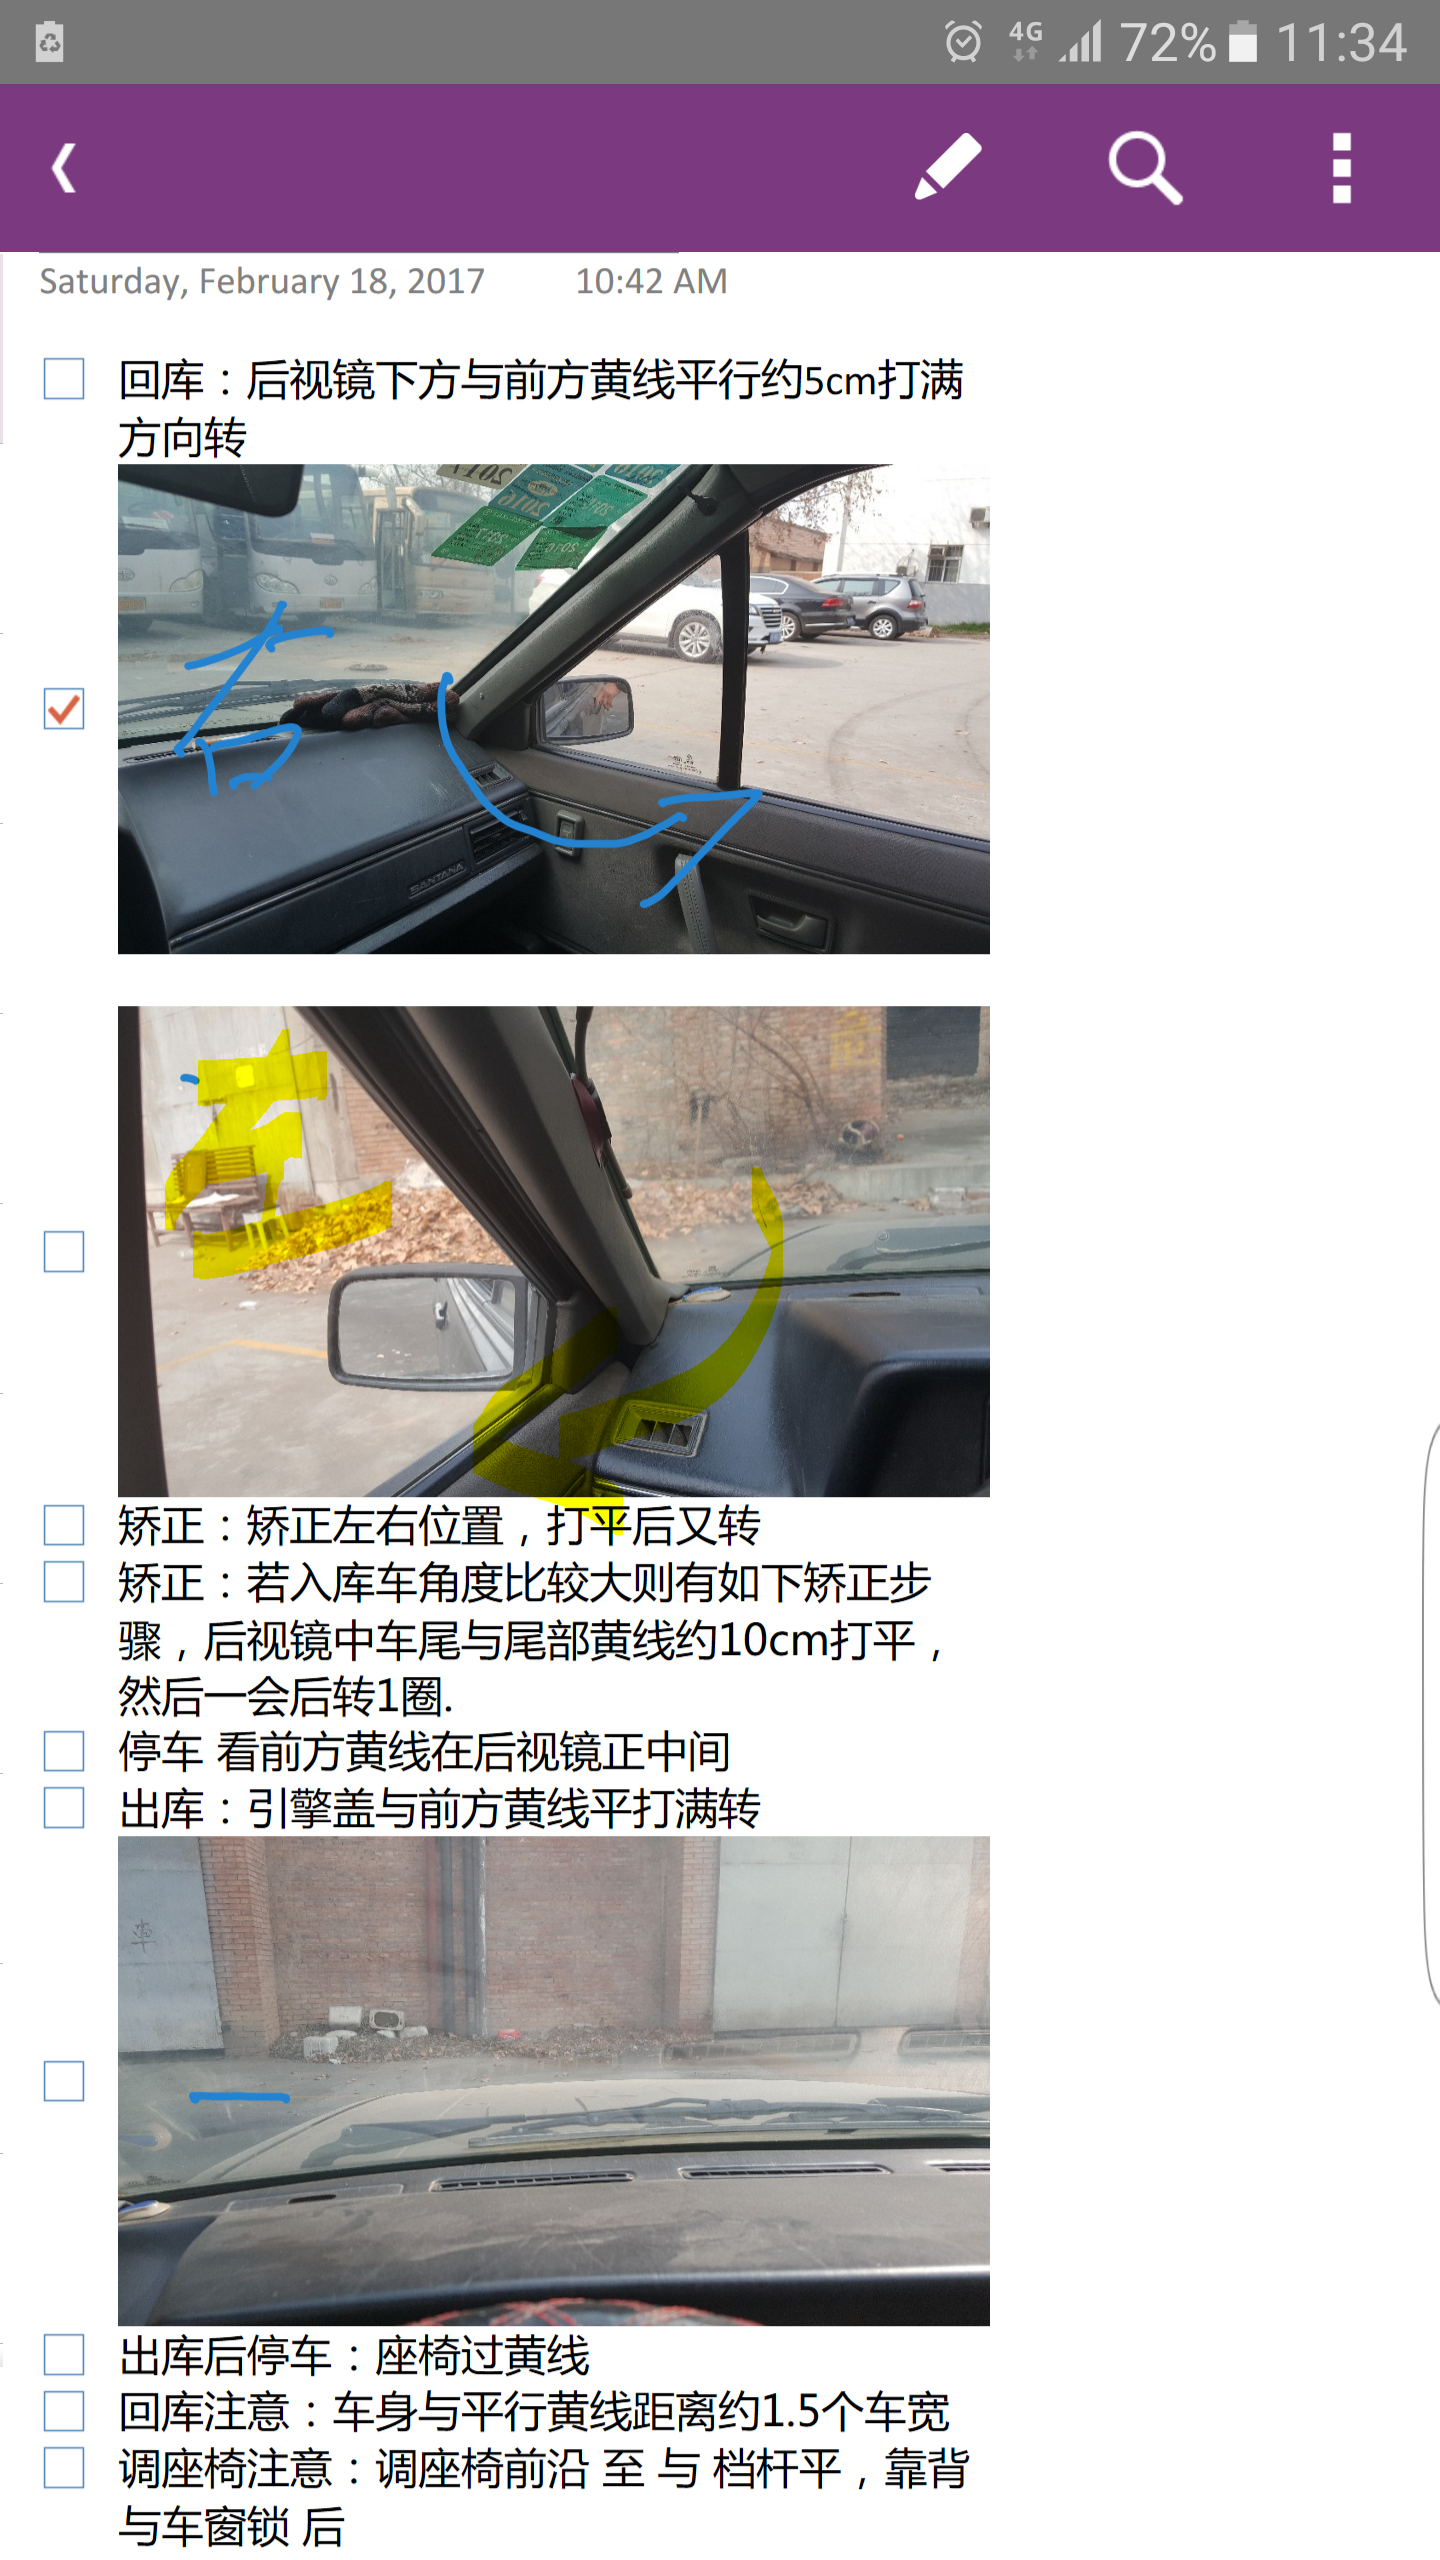
\includegraphics[scale = 0.2]{Drive.png}
		 		\caption{学车笔记}
		 		\label{Driver}
		 	\end{figure}
	 	 教练还反复的夸了我..给爸妈打了电话..
	 	  
	 	 下午学了会习,把linux 和 Git 搞定了..
	 	 
	 	 4 点左右继续去学车..知道了干红的干系列是几乎不含糖的红酒,干白是用白葡萄酿的..比较甘醇..等
	 	 
	 	 回来的路上给爷爷打了电话..爷爷在2姑家,听到我的电话还是挺开心的好像..
	 	 
	 	 下午吃了饭后,就不知道要干什么了..看了一节深度遍历..
	 	 
	 	 然后晚上就跑毛了..
	 	 
	 	 \begin{itemize}
	 	  	% 重要
	 	  	\item  \makebox[0pt][l]{$\square$}\raisebox{.15ex}{\hspace{0.1em}$\checkmark$} Linux 命令 - ps -a,x,u; kill
	 	  	
	 	  	% 较重要
	 	  	\item  \makebox[0pt][l]{$\square$}\raisebox{.15ex}{\hspace{0.1em}$\checkmark$} 读书  30 Mins		 	 
	 	  	\item  \makebox[0pt][l]{$\square$}\raisebox{.15ex}{\hspace{0.1em}$\checkmark$} Algorithm 思路
	 	  	\item  \makebox[0pt][l]{$\square$}\raisebox{.15ex}{\hspace{0.1em}$\checkmark$} C++ Git版本管理 版本回滚一节:并超额完成分支的学习
	 	  	
	 	  	% Habits
	 	  	\item  曾国潘家书 一节:一曰\textbf{看生书宜求速},不多读则太陋;一曰\textbf{温旧书宜求熟},不背诵则易忘;一曰\textbf{习字宜有恒},不善写则如身之无衣,山之无木;一曰\textbf{作文宜苦思},不善作则如人之哑不能言,马之肢不能行。\textbf{四者缺一不可,盖阅历一生深知之},深悔之者,今亦望家中诸侄力行之
	 	  	
	 	  	\item  \makebox[0pt][l]{$\square$}\raisebox{.15ex}{\hspace{0.1em}$\checkmark$} Topic- 史上最忠贞的爱情
	 	 \end{itemize}
	 	 
	 	 \textbf{切勿以家中有事而间断看书之课,又弗以考试将近而间断看书之课。虽走路之日,到店亦可看;考试之日,出场亦可看也}
 	 \paragraph{Day 19  学车第2天   \quad     }
	 	 Hello :
	 	 
	 	 早上依旧是小喵叫我起床的..8点左右离开宿舍..10点左右练上车..11点回到宿舍..点了外卖,吃了份炒面..
	 	 
	 	 下午去的比较早13:40 左右吧,然后竟然还是第四位..学了一把就走了..
	 	 
	 	 回来后把宿舍整理了下.. 然后把Linux 的环境一章略看了下..算是粗略有个眉目了..
	 	 
	 	 跟小喵聊天的时候..李飞回来了..然后决定晚上搓顿
	 	 \begin{itemize}
	 	 	% 重要
	 	 	\item  \makebox[0pt][l]{$\square$}\raisebox{.15ex}{\hspace{0.1em}$\checkmark$} Linux 命令 - \verb|PATH|
	 	 	\item  \makebox[0pt][l]{$\square$}\raisebox{.15ex}{\hspace{0.1em}$\checkmark$} C++ 内存模型 一节
	 	 	
	 	 	% 较重要
	 	 	\item  \makebox[0pt][l]{$\square$}\raisebox{.15ex}{\hspace{0.1em}$\checkmark$} 读书  30 Mins		 	 
	 	 	\item  \makebox[0pt][l]{$\square$}\raisebox{.15ex}{\hspace{0.1em}$\checkmark$} Algorithm - 挑战程序设计1节 1题
	 	 	\item  \makebox[0pt][l]{$\square$}\raisebox{.15ex}{\hspace{0.1em}$\checkmark$} muduo 一节:git remote clone
	 	 	\item  Net 一节
	 	 	\item  OS  一节
	 	 	
	 	 	% Habits
	 	 	\item  \makebox[0pt][l]{$\square$}\raisebox{.15ex}{\hspace{0.1em}$\checkmark$} Topic- 曾国藩(Fan) 巨蟒转世
	 	 \end{itemize}
 	 \paragraph{Day 20  学车第3天    \quad     }
	 	 早上起的挺早,但是前面还是有4个人竟然..
	 	 
	 	 学了一把..回,实在太冷了..
	 	 
	 	 下午学了vi,看了 c++ virtual 内存模型
	 	 
	 	 了解了 TCP,区分了 Epoll LT 和 ET 触发模式
	 	 \begin{itemize}
	 	 	% 重要
	 	 	\item  \makebox[0pt][l]{$\square$}\raisebox{.15ex}{\hspace{0.1em}$\checkmark$} Linux 命令 - vi编辑器:\verb|yy,dd,p,'\',n|
	 	 	\item  \makebox[0pt][l]{$\square$}\raisebox{.15ex}{\hspace{0.1em}$\checkmark$} C++ 内存模型 一节:virtual table
 and virtual ptr 	 	 	
	 	 	% 较重要
	 	 	\item  \makebox[0pt][l]{$\square$}\raisebox{.15ex}{\hspace{0.1em}$\checkmark$} 读书  30 Mins	:曾国藩家书 - 交友篇	 	 
	 	 	\item  \makebox[0pt][l]{$\square$}\raisebox{.15ex}{\hspace{0.1em}$\checkmark$} Algorithm - 挑战程序设计1节 1题
	 	 	\item  muduo 一节
	 	 	\item  \makebox[0pt][l]{$\square$}\raisebox{.15ex}{\hspace{0.1em}$\checkmark$} Net 一节 :TCP 3次握手理论,4次握手理论
	 	 	\item  OS  一节
	 	 	
	 	 	% Habits
	 	 	\item  \makebox[0pt][l]{$\square$}\raisebox{.15ex}{\hspace{0.1em}$\checkmark$} Topic- \textbf{秦淮八艳之一柳如是}
	 	 \end{itemize}
 	 \paragraph{Day 21  学车第4天    \quad     }Hello:
	 	 雨夹雪的天气学车你可想而知,倒库水面反光,等待又要淋雨..
	 	 
	 	 所以下午就没有去..
	 	 
	 	 看了2集红楼梦,学了会Linux..看懂了Thread pool如何更换任务的
	 	 
	 	 晚上刘斌老师请客吃了饭..得知他是搞并行计算与分布式计算的
	 	 
	 	 而且魏拓说明日早上会来..
	 	 
	 	 跟刘老师吃完饭后,突然对这个自己的论文题目有了些想法,可以搞定了应该..点云精简+重建+Reshape,主要是这个PCL 确实难装..但是最后还是攻下了..可喜可贺
	 	 
	 	 跟小喵的聊天成了每日的习惯..
 	 
	 	 \begin{itemize}
	 	 	% 重要
	 	 	\item  \makebox[0pt][l]{$\square$}\raisebox{.15ex}{\hspace{0.1em}$\checkmark$} Linux 命令 :ftp,netstat,ssh
	 	 	\item  \makebox[0pt][l]{$\square$}\raisebox{.15ex}{\hspace{0.1em}$\checkmark$} C++ :Thread pool
	 	 		 	 	
	 	 	% 较重要
	 	 	\item  \makebox[0pt][l]{$\square$}\hspace{1em} 读书  30 Mins	:	 	 
	 	 	\item  \makebox[0pt][l]{$\square$}\raisebox{.15ex}{\hspace{0.1em}$\checkmark$} Algorithm - 挑战程序设计1节 1题: 
	 	 	\item  muduo 一节
	 	 	\item  \makebox[0pt][l]{$\square$}\raisebox{.15ex}{\hspace{0.1em}$\checkmark$} Net 一节 :SSH
	 	 	\item  OS  一节
	 	 	
	 	 	% Habits
	 	 	\item  \makebox[0pt][l]{$\square$}\raisebox{.15ex}{\hspace{0.1em}$\checkmark$} Topic : 时间概念
	 	 \end{itemize}
	 	 
 	 \paragraph{Day 22  学车第5天    \quad     }Hello:
	 	 
		  早上起来7点左右(魏拓回来了)..去学车。今天教练没有在旁边指导,自己摸索的倒库..感觉找到了打点的要领..
		  
		  下午回来整理了一会Linux 和 Effective C++ 然后就去打球了..
		  
		  哦,魏拓给我了条他穿不了的牛仔裤子..听他说499呢..但是胖了穿不上了..自己应该感恩
		  
		  晚上洗了澡 和 7人帮去 码头故事吃了火锅..
		  
		  记笔记碎觉
	 	  \begin{itemize}
	 	  	% 重要
	 	  	\item  \makebox[0pt][l]{$\square$}\raisebox{.15ex}{\hspace{0.1em}$\checkmark$} Linux 命令 :Find locate
	 	  	\item  \makebox[0pt][l]{$\square$}\raisebox{.15ex}{\hspace{0.1em}$\checkmark$} C++ :Effective
	 	  	
	 	  	% 较重要
	 	  	\item   读书  30 Mins	:	 	 
	 	  	\item   Algorithm - 挑战程序设计1节 1题: 
	 	  	\item   muduo 一节 :
	 	  	\item   Net 一节 :
	 	  	\item   OS  一节 :
	 	  	
	 	  	% Habits
	 	  	\item  \makebox[0pt][l]{$\square$}\hspace{1em} Topic :
	 	  \end{itemize}
 	 \paragraph{Day 23  学车第6天    \quad   预约了下周5的考试  }Hello:
 	 
	 	 早上起床7点多..起床后去学车..着衣单薄..冷
	 	 
	 	 练车的时候车多次出现故障导致最后练车的时间一直延后..但还好今天预约了下周的科二考试..
	 	 
	 	 下午回啦把 Effective C++ 的相关 性能方面的书整理成册..然后睡了1个半多小时的午觉..起来后就开始整理,并完成对LINUX 的rsync 的学习
	 	 
	 	 晚上看了几集 红楼梦.. 对 宝玉与黛玉之间 的感情细节的描绘让我不禁赞叹..情中方可体其味
	 	 
	 	 然后整理了 计算机网络的相关知识.. C++ 的Trace 类之类的技巧.. 以及引用技术的概念等.. 睡
	 	 
	 	 \begin{itemize}
	 	 	% 重要
	 	 	\item  \makebox[0pt][l]{$\square$}\raisebox{.15ex}{\hspace{0.1em}$\checkmark$} Linux 命令 :rsync, Find
	 	 	\item  \makebox[0pt][l]{$\square$}\raisebox{.15ex}{\hspace{0.1em}$\checkmark$} C++ :Effective One Section
	 	 	
	 	 	% 较重要
	 	 	\item   读书  30 Mins	:	 	 
	 	 	\item  \makebox[0pt][l]{$\square$}\raisebox{.15ex}{\hspace{0.1em}$\checkmark$} Algorithm - 挑战程序设计1节 1题:最多排课 
	 	 	\item   muduo 一节 :
	 	 	\item  \makebox[0pt][l]{$\square$}\raisebox{.15ex}{\hspace{0.1em}$\checkmark$} Net 一节 :计算机网络性能的计算与理论
	 	 	\item  \makebox[0pt][l]{$\square$}\raisebox{.15ex}{\hspace{0.1em}$\checkmark$} OS  一节 : 1 section- 基本概念-层次与模块
	 	 	
	 	 	% Habits
	 	 	\item  \makebox[0pt][l]{$\square$}\raisebox{.15ex}{\hspace{0.1em}$\checkmark$} Topic :古代的厕纸
	 	 \end{itemize}
 	 \paragraph{Day 24  分教练了    \quad     }Hello:
 	 
	 	 早上起来上了厕所后,到达练车的地方就晚了些.. 但是庆幸的是今天终于正儿八经的正式登记了周5的考试了..
	 	 
	 	 早上练了7圈..学会了带刹车的起步..
	 	 
	 	 下午补充了午觉,出校门看了小喵..她沧桑了..真为她担心..该怎么结束呢?
	 	 
	 	 下午与李飞和魏拓一起下山去吃 茴香阁的泡馍去了..回来好好的看了 Effective C++ 的相关知识 并看完 了提高C++ 编程技术一书和 Effective STL 
	 	 ,但是 这些只是粗读,只是了解而并非是深入研究.
	 	 
	 	 晚上看了 OS 和 Net 相关知识,并把曾国藩家书略读了几节..反思了今日之事..
	 	 \begin{itemize}
	 	 	% 重要
	 	 	\item  \makebox[0pt][l]{$\square$}\raisebox{.15ex}{\hspace{0.1em}$\checkmark$} Linux 命令 :找到一份Linux 的熟练程度对比手册
	 	 	\item  \makebox[0pt][l]{$\square$}\raisebox{.15ex}{\hspace{0.1em}$\checkmark$} C++ :Effective C++
	 	 	
	 	 	% 较重要
	 	 	\item  \makebox[0pt][l]{$\square$}\raisebox{.15ex}{\hspace{0.1em}$\checkmark$} 读书  30 Mins	:麦田守望者	 	 
	 	 	\item  \makebox[0pt][l]{$\square$}\hspace{1em} Algorithm - 1节 1题:
	 	 	\item  \makebox[0pt][l]{$\square$}\raisebox{.15ex}{\hspace{0.1em}$\checkmark$} Net 一节 :应用层 部分协议与应用
	 	 	\item  \makebox[0pt][l]{$\square$}\raisebox{.15ex}{\hspace{0.1em}$\checkmark$} OS  一节 :PCB
	 	 	
	 	 	% Habits
	 	 	\item  \makebox[0pt][l]{$\square$}\raisebox{.15ex}{\hspace{0.1em}$\checkmark$} 曾国藩(Fan)家书一节: \textbf{未有主帅晏而将弁能早者也,犹之一家之中,未能家长晏而子弟能早者也.} 
	 	 	
	 	 	\textbf{家中读书事,弟宜常常留心,如甲五科三等,皆须读书,不失大家子弟风范,不可太疏忽也}.
	 	 	
	 	 	\textbf{诸侄不知俭约者,常常训责之否?}
	 	 	\item  \makebox[0pt][l]{$\square$}\raisebox{.15ex}{\hspace{0.1em}$\checkmark$} Topic :“跳槽”的来历
	 	 \end{itemize}
 	 \paragraph{Day 25  分到李国庆了   \quad   但是他的通过率好低呀  }Hello:\
 	 
	 	 早上起床又略偏晚.. 然后在练倒库的2楼分了我们的李教练..刚开始知道他的通过率特别低,然后心里就特别慌,然而他的人少呢..练得圈数多呢
	 	 
	 	 走时最后,去的又最晚.. 让我们的感觉是他非常的不负责人,虽然下午该记的点都记了,但是最后还是第一个走的..
	 	 
	 	 晚上回来约了明天约会小喵.. 然后看了 C++ 和 Net 的相关知识
 	 
	 	 \begin{itemize}
	 	 	% 重要
	 	 	\item  \makebox[0pt][l]{$\square$}\hspace{1em} Linux 命令 :Grep
	 	 	\item  \makebox[0pt][l]{$\square$}\hspace{1em} C++ :继承与面向对象设计一节
	 	 	
	 	 	% 较重要
	 	 	\item  \makebox[0pt][l]{$\square$}\raisebox{.15ex}{\hspace{0.1em}$\checkmark$} 读书  30 Mins	:The Catcher in the Rye	 	 
	 	 	\item  \makebox[0pt][l]{$\square$}\hspace{1em} Algorithm - 1节 1题:
	 	 	\item  \makebox[0pt][l]{$\square$}\raisebox{.15ex}{\hspace{0.1em}$\checkmark$} Net 一节 :端口+UDP
	 	 	%\item  \makebox[0pt][l]{$\square$}\raisebox{.15ex}{\hspace{0.1em}$\checkmark$} OS  一节 :
	 	 	
	 	 	% Habits
	 	 	%\item  \makebox[0pt][l]{$\square$}\raisebox{.15ex}{\hspace{0.1em}$\checkmark$} 曾国藩(Fan)家书一节:
	 	 	\item  \makebox[0pt][l]{$\square$}\raisebox{.15ex}{\hspace{0.1em}$\checkmark$} Topic :北宋词人张先
	 	 \end{itemize}
 	 \paragraph{Day 26      \quad     }Hello:
 	 
	 	 早上起床7:30 洗脸离开宿舍7:42- 7:48到.. 去了后学了4圈就让教练撵回来了..
	 	 
	 	 下午和晚上陪小喵了
	 	 
	 	 下午先是去 川渝府 吃饭,点了小炒木耳和豆角茄子..喝了粟米粥..
	 	 
	 	 然后去了水运中心,坐在那个中间的高台阶上看着远方天上的风筝..她就在这时亲了我的脸颊..
	 	 
	 	 然后我们一路走回到怡家然后看了 生化危机 电影.
	 	 
	 	 然后回宾馆你懂的..就是简单的抱着她就好..
	 	 
	 	 非要起床去吃李想大虾,吃就吃呗..小喵进步了呢..撒的不那么严重了
 	 \paragraph{Day 27  学车第9天了   \quad     }Hello:
	 	 
	 	 晚上一直抱着小喵,一分一秒都紧贴着彼此..
	 	 
	 	 然后离开宾馆我就坐车去了驾校.. 20元呢..到了驾校向一位大姐借了纸先是冲去上厕所了..
	 	 
	 	 下午回来也没休息,也没学习..看了些许电影..然后也不知干了什么接着就去西区吃饭了.
	 	 
	 	 晚上回来把中午美丽姐发的进度情况好好反思了一番,然后开始琢磨用 \verb|PCL |如何实现这个的问题..最后在11点将近时终于完成了..
	 	  
 	 \paragraph{Day 28  学车第10日了    \quad  星期二、再可以练习2天了   }Hello:
 	 
	 	 可是今天早上的S 弯道出现错误了
	 	 
	 	 下午睡到16点左右,看了两节 麦田的守望者..
	 	 
	 	 晚上阿妈发来 苦涩的辛酸谈吐..一切的压力又重回肩上,该当家了..
	 	 
	 	 所以得全力以赴了.. 	 
	 	 \begin{itemize}
	 	 	% 重要
	 	 	\item  \makebox[0pt][l]{$\square$}\raisebox{.15ex}{\hspace{0.1em}$\checkmark$} Linux 命令复习 :
	 	 	\item  \makebox[0pt][l]{$\square$}\hspace{1em} C++ :继承与面向对象设计一节
	 	 	
	 	 	% 较重要
	 	 	\item  \makebox[0pt][l]{$\square$}\raisebox{.15ex}{\hspace{0.1em}$\checkmark$} 读书  30 Mins	:The Catcher in the Rye	 	 
	 	 	\item  \makebox[0pt][l]{$\square$}\hspace{1em} Algorithm - 1节 1题:
	 	 	\item  \makebox[0pt][l]{$\square$}\hspace{1em} Net 一节 :
	 	 	%\item  \makebox[0pt][l]{$\square$}\raisebox{.15ex}{\hspace{0.1em}$\checkmark$} OS  一节 :
	 	 	
	 	 	% Habits
	 	 	\item  \makebox[0pt][l]{$\square$}\raisebox{.15ex}{\hspace{0.1em}$\checkmark$} 曾国藩(Fan)家书 修身 一节:
		 	 	格物,致知之事也; 诚意,例行之事也
		 	 	
		 	 	一日之中,一念之差,一事之失,一言一默
		 	 	
		 	 	若读书不能体贴到身上去,此谓三项,与我身毫不相涉,则读书何用?
		 	 	
		 	 	且苟能发奋自立,则家塾可读书,即旷野之地,热闹之场,亦可读书,负薪牧啄,皆可读书;苟不能发奋自立,则家塾不能读书,即清静之乡,神仙之境皆不能读书。何必择地?何必择时?但自问立志之真不真耳!
		 	 	
		 	 	所谓诚意者,即其所知而力行之,是不欺也,知一句便行一句
	 	 	\item  \makebox[0pt][l]{$\square$}\raisebox{.15ex}{\hspace{0.1em}$\checkmark$} Topic :清朝皇帝龙袍值多少钱
	 	 \end{itemize}
	 	 
 	\paragraph{Month Summary}
 	 
 \section{March}
 	 \paragraph{Day 1  再有一天考试了     \quad     }Hello :
 	 
	 	 \verb|C++ | 书单
		 	 \begin{itemize}[itemindent = 2em]
		 	 	\item \verb|Profession C++|
		 	 	\item \verb|Effective C++/ And More/ And Modern/ And STL|
		 	 	\item \verb|Exception/ And More|
		 	 	\item \verb|编写可读代码的艺术|
		 	 \end{itemize}
	 	 
	 	 \verb|Net | 书单
		 	 \begin{itemize}[itemindent = 2em]
		 	 	\item \verb|计算机网络|
		 	 	\item \verb|构建高性能服务器|
		 	 	\item \verb|boost.AsyncIO Network Programming|
		 	 	\item \verb|Muduo|
		 	 \end{itemize}
	 	 
	 	 \verb|面试 | 书单
		 	 \begin{itemize}[itemindent = 2em]
		 	 	\item \verb|Datastructure|
		 	 	\item \verb|OperatorSystem|
		 	 	\item \verb|剑指Offer|
		 	 	\item \verb|LeetCode 题解|
		 	 \end{itemize}
		 	
		 早上起床照例去了驾校.. 把S弯道终于搞定了.. 进的时候是压一般道岩,出的时候是压1/4 个道岩。
		 
		 回来看了部电影就出去取我的身份证了.. 陪小喵看了看包.. 但是只买了双鞋..
		 
		 下午回来的路上给阿爸和阿妈都沟通了好长时间..心烦的很
		 
		 晚上看了会儿C++ Professional 和 Effective C++.. 然后又学不进去了..
		 
		 好多任务都没完成..心情好烦呢.. 
	 	 \begin{itemize}
	 	 	% 重要
	 	 	\item  \makebox[0pt][l]{$\square$}\hspace{1em} Linux 命令复习 :
	 	 	\item  \makebox[0pt][l]{$\square$}\raisebox{.15ex}{\hspace{0.1em}$\checkmark$} C++ Effective 5-items:继承与面向对象设计一节
	 	 	
	 	 	% 较重要
	 	 	\item  \makebox[0pt][l]{$\square$}\raisebox{.15ex}{\hspace{0.1em}$\checkmark$} 读书  30 Mins	:The Catcher in the Rye	 	 
	 	 	\item  \makebox[0pt][l]{$\square$}\hspace{1em} Algorithm - 1节 1题:
	 	 	\item  \makebox[0pt][l]{$\square$}\hspace{1em} Net 一节 :
	 	 	%\item  \makebox[0pt][l]{$\square$}\raisebox{.15ex}{\hspace{0.1em}$\checkmark$} OS  一节 :
	 	 	
	 	 	% Habits
	 	 	%\item  \makebox[0pt][l]{$\square$}\raisebox{.15ex}{\hspace{0.1em}$\checkmark$} 曾国藩(Fan)家书 修身 一节:
	 	 	\item  \makebox[0pt][l]{$\square$}\raisebox{.15ex}{\hspace{0.1em}$\checkmark$} Topic :
	 	 \end{itemize}
 	 \paragraph{Day 2  明天考试     \quad     }
	 	 Hello:
	 	 
	 	 坚持了数日,感觉最近又有昏睡之势头,需提防
	 	 
	 	 早上学了最后一天的科目二,希望明天可以顺利通过..早日完成驾照事宜..
	 	 
	 	 下午睡了些许,感觉起床后精神好多了,看起书来也是乘风破浪..
	 	 
	 	 晚间,赵泽光打来电话说要订婚..甚是欣喜,好友还是好友,虽常不联系,记的就好..他3月16日于槐柏订婚。
	 	 
	 	 午间,与李飞开玩笑等谈吐之时,因过于高兴却忘记开玩笑度的问题..搞的对方很不开心,失去了本来开玩笑的目的,这是个很不好的兆头,所以玩笑归玩笑,亦须有度。
	 	 
	 	 晌午,陪小喵发传单..看着她的小脸尚是担忧..愿好转。
	 	 \begin{itemize}[itemindent = 1em]
	 	 	\renewcommand\labelitemi{\makebox[0pt][l]{$\square$}\raisebox{.15ex}{\hspace{0.1em}$\checkmark$}}
	 	 	% 重要
	 	 	\item   Linux 命令复习 :如何布置服务器
	 	 	\item   C++ Effective 5-items:\verb|Class Name and Initializer-List|
	 	 	
	 	 	% 较重要
	 	 	\item   读书  30 Mins	:\verb|The Catcher in the Rye	| 
	 	 	\item   Net 一节 :\verb|IP 分类|	
	 	 	\item   Algorithm - 1节 1题:\verb|蓝桥3题|
	 	 	%\item  OS  一节 :
	 	 	
	 	 	\renewcommand\labelitemi{\makebox[0pt][l]{$\square$}\raisebox{.15ex}{\hspace{0.1em}$\checkmark$}}
	 	 	% Habits
	 	 	\item  曾国藩(Fan)家书 修身 一节:大抵第一要\textbf{除骄傲之气,中无所有,而夜郎自大,此最坏事}。求大人教六弟,总期不自满足为要。
	 	 	\item   Topic :小蛮腰到底是谁的腰
	 	 \end{itemize}
 	 \paragraph{Day 3  科2考过了    \quad     }
	 	  Hello:
	 	  
	 	  从早上起床(7:20)洗了头就为开始开始操心,担心得等到中午没饭吃,特地的吃了早饭..
	 	  
	 	  可是在等待考试的途中紧张的一直想上厕所..卖了纸排了堆积了几天的粪便,想想也是对身体有益..
	 	  
	 	  中午时分(11:30)得知需要等待半个小时,此时出去发现餐馆吃了午饭..然后又在焦急的等待.. 一个接一个的考试的人顺利通过..心里又担心又高兴..我们这一批的都过了..  可是屏幕还是始终不出现我的名字.. 是不是出错了呢,信息没录上? 各种想法浮现在脑海中.. 到最后只剩下我一个人没出现在屏幕上时..忐忑的你简直不敢相信这个心已经跳到天上去 了..
	 	  
	 	  进去后还是最后一个(14:50 左右).. 等待着.. 5号车.. 满分过!激动与喜悦的情绪始终无法掩盖..
	 	  
	 	  回来后联系了教练报了喜讯,约了科目三的训练.. 尽快拿下驾照.这件事
	 	  
	 	  晚间放松看了几部电影,与饱凤聊了些许.. 与小喵中午的聊天不知最后怎么炎炎了之..
	 	  
	 	  \textbf{填空题没有什么不可以用暴力破解的..}
	 	  \begin{itemize}[itemindent = 1em]
	 	  	\renewcommand\labelitemi{\makebox[0pt][l]{$\square$}\raisebox{.15ex}{\hspace{0.1em}$\checkmark$}}
	 	  	% 重要
	 	  	\item   Linux 命令复习 :\verb|GDB Linux|  调试
	 	  	\item   C++ Effective 5-items:\verb|Professional C++ Chapter8|
	 	  	
	 	  	% 较重要
	 	  	\item   读书  30 Mins	:\verb|The Catcher in the Rye|	
	 	  	\renewcommand\labelitemi{\makebox[0pt][l]{$\square$}\hspace{1em}} 
	 	  	\item   Net 一节 :IP 子网掩码	
	 	  	\item   Algorithm - 1节 1题:
	 	  	%\item  OS  一节 :
	 	  	
	 	  	\renewcommand\labelitemi{\makebox[0pt][l]{$\square$}\raisebox{.15ex}{\hspace{0.1em}$\checkmark$}}
	 	  	% Habits
	 	  	%\item  曾国藩(Fan)家书 修身 一节:
	 	  	\item   Topic :七不责
	 	  \end{itemize}
 	 \paragraph{Day 4  科目3开始练习了    \quad     }Hello:
 	 
	 	 早上起床跑错了位置,到了科目2的考场才知道是在东辉的倒库场地报名..又走回来了..跟张越佳 在李教练的手下进行练习科目3
	 	 
	 	 回来看了两眼书就睡觉了..困
	 	 
	 	 起床后,李飞与魏拓 已将快递取回并吃了午饭.. 而李飞 将仅有的两盒 洁面赠品给了 我与魏拓,而最值得学习的是.. 给我的这盒的时候他再有一盒了..\textbf{而他完全没有犹豫就将该 物品 送给了我}, \textit{要是我的话:肯定先是一顿牢骚,最后东西给了 然后留下 一场很不开心的结局,东西给了,而且没落下好..}; \textbf{所以这就是做事方式的差距}.. 
	 	 
	 	 这就是要学的.. 大方..有的时候吃点亏都无所谓.就害怕到最后练吃亏的机会都没有了..
	 	 
	 	 下午去了练科三的地方,把该记的点都记了.. 下周5进行考试..
 	 
	 	 \begin{itemize}[itemindent = 1em]
	 	 	\renewcommand\labelitemi{\makebox[0pt][l]{$\square$}\hspace{1em}} 
	 	 	% 重要
	 	 	\item   还书-续借
	 	 	\renewcommand\labelitemi{\makebox[0pt][l]{$\square$}\raisebox{.15ex}{\hspace{0.1em}$\checkmark$}}
	 	 	\item   Linux 命令复习 :\verb|GDB Linux|  调试
	 	 	\item   C++ Effective 5-items:\verb|Professional C++ Chapter9-Override|
	 	 	
	 	 	% 较重要
	 	 	\item   读书  30 Mins	:\verb|The Catcher in the Rye|	
	 	 	\renewcommand\labelitemi{\makebox[0pt][l]{$\square$}\hspace{1em}} 
	 	 	\item   Net 一节 :IP 子网掩码	
	 	 	\item   Algorithm - 1节 1题:
	 	 	%\item  OS  一节 :
	 	 	
	 	 	\renewcommand\labelitemi{\makebox[0pt][l]{$\square$}\raisebox{.15ex}{\hspace{0.1em}$\checkmark$}}
	 	 	% Habits
	 	 	\item  曾国藩(Fan)家书 修身 一节: \textbf{非知之艰,行之维艰}..(不是认识事物难,而是认识了去实现更难)
	 	 	
	 	 	\textbf{但不能庄严威厉,使人望若神明耳}..(但为人不能太严肃厉害,使人像望着神明一样..)
	 	 	
	 	 	傲气既长,终不进功,所以潦倒一生,而无寸进也。
	 	 	
	 	 	余平生科名极为顺遂,惟小考七次始售。\textbf{然每次不进,未尝敢出一怨言,但深愧自己试场之诗文太丑而已}。至今思之,如芒在背。当时之不敢怨言,诸弟问父亲、叔父及朱尧阶便知。盖场屋之中,\textbf{只有文丑而侥幸者,断无文佳而埋没者,此一定之理也}
	 	 	
	 	 	故\textbf{吾人用功,力除傲气,力戒自满,毋为人所冷笑,乃有进步也}
	 	 	
	 	 	弟累年\textbf{小试不售},\textit{恐因愤激之久,致生骄惰之气,故特作书戒之}
	 	 	\item   Topic : 驸马苦逼的生活: 外亲干政-事业退, 皇家女儿娇生惯养-家乱, 而且还不一定美..而且是皇室不能欺君
	 	 \end{itemize}
 	 \paragraph{Day 5  科目3练习第2天    \quad     }
	 	 
	 	 早上练习了4圈..下午打了会球、洗了澡..
	 	 
	 	 \textbf{制定的任务就留给明天吧}--这样会不会不太好
	 	 
	 	 整理了 科目3 行程图
		 	 \begin{figure}[h]
		 	 	\centering
		 	 	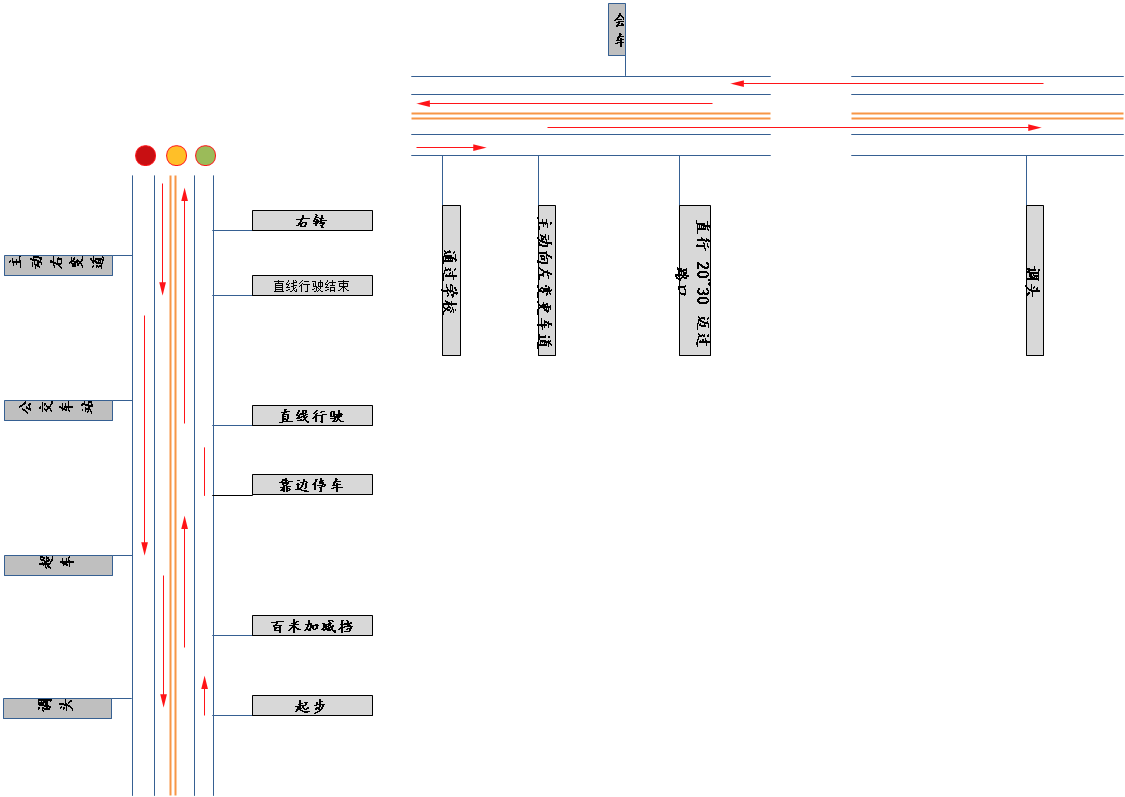
\includegraphics[scale = 0.4]{license3.png}
		 	 \end{figure}
	 	
 	 \paragraph{Day 6  休息     \quad     }Hello :
 	 
	 	 晚上这些货(晓东、存宝、魏拓)打王者荣耀声音大的搞得睡觉都是装着满肚子的不满..
 	 
	 	 下午又开始练车了..
 	 
	 	 晚上订了 明天去虹桥 吃火锅
	 	 \begin{itemize}[itemindent = 1em]
	 	 	\renewcommand\labelitemi{\makebox[0pt][l]{$\square$}\hspace{1em}} 
	 	 	% 重要
	 	 	\renewcommand\labelitemi{\makebox[0pt][l]{$\square$}\raisebox{.15ex}{\hspace{0.1em}$\checkmark$}}
	 	 	\item   还书-续借	 	 	
	 	 	\item   Linux 命令复习 :
	 	 	\item   C++ Effective 5-items:\verb|Professional C++ Chapter9-切片|
	 	 	
	 	 	% 较重要
	 	 	\item   读书  30 Mins	:\verb|The Catcher in the Rye|	
	 	 	\renewcommand\labelitemi{\makebox[0pt][l]{$\square$}\hspace{1em}} 
	 	 	\item   Net 一节 :IP 子网掩码	
	 	 	\item   Algorithm - 1节 1题:
	 	 	%\item  OS  一节 :
	 	 	
	 	 	\renewcommand\labelitemi{\makebox[0pt][l]{$\square$}\raisebox{.15ex}{\hspace{0.1em}$\checkmark$}}
	 	 	% Habits
	 	 	\item  曾国藩(Fan)家书 修身 一节: 做事当不苟不懈: 男虽终身在礼部衙门,为国家办照例之事,不苟不懈,尽就条理,易所深愿也。(丝毫不敢马虎松懈,一概按规矩办理)
	 	 	\item   Topic : 
	 	 \end{itemize}
 	 \paragraph{Day 7  学车第4天     \quad     }Hello:
	 	 
		 早上练习了 6圈,然后通知明天练习1天..
		 
		 中午去虹桥吃了火锅..然后去大润 超市买了个杯子,在门口还抽了个一等奖..最后还是因为没钱没买
		 
		 下午回来就睡..
	 	 
	 	 晚上整理出来个简历框架..争取考完科三的时候简历弄完
 	 \paragraph{Day 8  全体学车     \quad     }
	 	 
	 	 早上吃了瘦肉加膜,然后买饮料被坑..估计不会再去了..门口右角
	 	 
	 	 练习了一天,下午回来又去练车,没想到第一把模拟就通过了..很高兴,今天练了9把吧..感觉还不错..希望后天可以顺利完成考试。
	 	 
	 	 晚上回来宿舍后,看了会Effective C++,整理了 \verb|iostream_iterator|,将More Effective C++ 条目摘抄了下..准备好好的复习了。
	 	 
	 	 感觉 边看面试题边复习更有针对性,但是广度还是不够,需要加强..
	 	 
	 	 下午给老妈发了祝福,给小喵发了红包..明天与小喵吃饭,但是写论文的计划好像被打乱的忘到九霄云外了..是时候提上日程了
 	 \paragraph{Day 9  休息     \quad     }
 	 
		  起床陪小喵吃了饭到川渔府..
		  
		  看了 狗的一生这部电影.. 
		  
		  回来后 睡了会,复习了Linux 通过视频,学习了网关的概念
		  
		  研究了会 采样算法..
		  
		  准备考试..
	 	  \begin{itemize}[itemindent = 1em]
	 	  	\renewcommand\labelitemi{\makebox[0pt][l]{$\square$}\hspace{1em}} 
	 	  	% 重要
	 	  	\renewcommand\labelitemi{\makebox[0pt][l]{$\square$}\raisebox{.15ex}{\hspace{0.1em}$\checkmark$}}	 	
	 	  	\item   Linux 命令复习 :\verb|grep find locate|
	 	  	\item   C++ Effective 5-items:\verb|Professional C++ Chapter9-切片|
	 	  	\item   完善 简历
	 	  	
	 	  	% 较重要
	 	  	\item   读书  30 Mins	:\verb|The Catcher in the Rye|	
	 	  	\item   Net 一节 :IP 子网掩码
	 	  	\renewcommand\labelitemi{\makebox[0pt][l]{$\square$}\hspace{1em}} 	
	 	  	%\item   Algorithm - 1节 1题:
	 	  	%\item  OS  一节 :
	 	  	
	 	  	\renewcommand\labelitemi{\makebox[0pt][l]{$\square$}\raisebox{.15ex}{\hspace{0.1em}$\checkmark$}}
	 	  	% Habits
	 	  	%\item  曾国藩(Fan)家书 修身 一节:
	 	  	\item   Topic : 
	 	  \end{itemize}
 	 \paragraph{Day 10 考试 科目三考过了.  \quad     }Hello:
 	 
	 	 昨个睡得早..早上7点就起床了..偷了绿色能量就去蹭“白富美-张越佳” 的滴滴车了..
	 	 
	 	 等着等着轮到我考试了呢...激动的以为会在灯光上还有百米加减档掉下去..后来在直线行驶上上了40把我吓得以为要挂..最后成绩合格时把我激动的..
	 	 
	 	 晚上吃了 川渝府私家菜.. 他们评价一般
 	 \paragraph{Day 11      \quad     }
	 	 \begin{itemize}[itemindent = 1em]
	 	 	\renewcommand\labelitemi{\makebox[0pt][l]{$\square$}\hspace{1em}} 
	 	 	% 重要
	 	 	\renewcommand\labelitemi{\makebox[0pt][l]{$\square$}\raisebox{.15ex}{\hspace{0.1em}$\checkmark$}}	 	
	 	 	\item   Linux 命令复习 :
	 	 	\item   C++ Effective 5-items:\verb|Professional C++ Chapter9-切片|
	 	 	\item   Sample Algorithm
	 	 	\item   完善 简历
	 	 	
	 	 	% 较重要
	 	 	\item   读书  30 Mins	:\verb|The Catcher in the Rye|	
	 	 	\renewcommand\labelitemi{\makebox[0pt][l]{$\square$}\hspace{1em}} 
	 	 	%\item   Net 一节 :	
	 	 	%\item   Algorithm - 1节 1题:
	 	 	%\item   OS  一节 :
	 	 	
	 	 	\renewcommand\labelitemi{\makebox[0pt][l]{$\square$}\raisebox{.15ex}{\hspace{0.1em}$\checkmark$}}
	 	 	% Habits
	 	 	%\item  曾国藩(Fan)家书 修身 一节:
	 	 	\item   Topic : 
	 	 \end{itemize}
 	 \paragraph{Day 12 晚上回家     \quad     }
 	 \paragraph{Day 13 郝楠订婚     \quad     }
 	 \paragraph{Day 14 家     \quad     }
 	 \paragraph{Day 15 家     \quad     }
 	 \paragraph{Day 16 文全订婚、回杨凌     \quad     }
 	 \paragraph{Day 17 回学校、写出了Sampling 程序   \quad     }
	 	 
 	 \paragraph{Day 18      \quad     }Hello:
 	 
	 	 早上起床就知道感冒了.. 起床后就开始加班赶工,把代码 从PCL的简化版本中往整体的框架中 融入,快接近中午吃饭时把大体的代码写完了..剩下的就是单纯的编译问题..
	 	 
	 	 64位的PCL 与 32 位 的Win32窗口... 最后智能PCL妥协了,安装了将近半个下午的环境,最后总算配好了..在魏拓出去打球的一个小时里把代码搞完了..
	 	 
	 	 晚上看了 C++ Effective 学习了2节吧.. 然后看了部叫《路易的9条命》 的电影
	 	 
	 	 睡觉
	 	 \begin{itemize}[itemindent = 1em]
	 	 	\renewcommand\labelitemi{\makebox[0pt][l]{$\square$}\hspace{1em}} 
	 	 	% 重要
	 	 	\renewcommand\labelitemi{\makebox[0pt][l]{$\square$}\raisebox{.15ex}{\hspace{0.1em}$\checkmark$}}	 	
	 	 	\item   Linux 命令复习 :
	 	 	\item   C++ Effective 5-items:\verb|隐身类型转换 与 new Operator with operator new|
	 	 	\item   Sample Algorithm: Totally Completed..
	 	 	\item   完善 简历
	 	 	
	 	 	% 较重要
	 	 	\item   读书  30 Mins	:\verb|当我们讨论跑步时讨论什么|	
	 	 	\renewcommand\labelitemi{\makebox[0pt][l]{$\square$}\hspace{1em}} 
	 	 	%\item   Net 一节 :	
	 	 	%\item   Algorithm - 1节 1题:
	 	 	%\item   OS  一节 :
	 	 	
	 	 	\renewcommand\labelitemi{\makebox[0pt][l]{$\square$}\raisebox{.15ex}{\hspace{0.1em}$\checkmark$}}
	 	 	% Habits
	 	 	\item  曾国藩(Fan)家书 修身 一节:幸息忍耐为要
	 	 	\item   Topic : 
	 	 \end{itemize}
 	 \paragraph{Day 19      \quad     }
 	 
	 	 \begin{itemize}[itemindent = 1em]
	 	 	\renewcommand\labelitemi{\makebox[0pt][l]{$\square$}\hspace{1em}} 
	 	 	% 重要
	 	 	\renewcommand\labelitemi{\makebox[0pt][l]{$\square$}\raisebox{.15ex}{\hspace{0.1em}$\checkmark$}}	 	
	 	 	\item   Linux 命令复习 :Linux 简介
	 	 	\item   C++ Effective 5-items:
	 	 	\item   Sampling  相关论文 理论
	 	 	\item   完善 简历
	 	 	
	 	 	% 较重要	
	 	 	\renewcommand\labelitemi{\makebox[0pt][l]{$\square$}\hspace{1em}} 
	 	 	\item   读书  30 Mins	:\verb|当我们讨论跑步时讨论什么|
	 	 	\item   Net 一节 :	
	 	 	%\item   Algorithm - 1节 1题:
	 	 	%\item   OS  一节 :
	 	 	
	 	 	\renewcommand\labelitemi{\makebox[0pt][l]{$\square$}\raisebox{.15ex}{\hspace{0.1em}$\checkmark$}}
	 	 	% Habits
	 	 	\item   曾国藩(Fan)家书 修身 一节:
	 	 	\item   Topic : 
	 	 \end{itemize}
		 	 今天一天算是废了.. 难受的根本看不进去..
	 	 
		 	 跟他们玩了一晚上王者荣耀
 	 \paragraph{Day 20      \quad     }
		 	 今天玩了一天的游戏.. 唉,需要预定计划并一步一步的执行了
 	 
	 	 
 	 \paragraph{Day 21  将CUDA的环境搞定    \quad     }
		 	 今天玩了一天的游戏..
		 	 
 	 \paragraph{Day 22  学CUDA   \quad     }Hello:
 	 
	 	 今天玩了多半天的游戏..
	 	 
	 	 下午4点开始学习.. 而且感冒好点了
	 	 
 	 \paragraph{Day 23      \quad     }
 	 
	 	 \begin{itemize}[itemindent = 1em]
	 	 	\renewcommand\labelitemi{\makebox[0pt][l]{$\square$}\hspace{1em}} 
	 	 	% 重要
	 	 	\renewcommand\labelitemi{\makebox[0pt][l]{$\square$}\raisebox{.15ex}{\hspace{0.1em}$\checkmark$}}	 	
	 	 	\item   Linux 命令复习 :系统分区
	 	 	\item   C++ Effective 5-items:\verb|Catch By Reference|
	 	 	\item   CUDA 剩下的..
	 	 	
	 	 	% 较重要
	 	 	\item   读书  30 Mins	:\verb|当我们讨论跑步时讨论什么|	
	 	 	\renewcommand\labelitemi{\makebox[0pt][l]{$\square$}\hspace{1em}} 
	 	 	%\item   Net 一节 :	
	 	 	%\item   Algorithm - 1节 1题:
	 	 	%\item   OS  一节 :
	 	 	
	 	 	\renewcommand\labelitemi{\makebox[0pt][l]{$\square$}\raisebox{.15ex}{\hspace{0.1em}$\checkmark$}}
	 	 	% Habits
	 	 	%\item   曾国藩(Fan)家书 修身 一节:
	 	 	\item   Topic : 
	 	 \end{itemize}
 	 \paragraph{Day 24      \quad     }
 	 
		 尝试.. 完成了 对于 CPP 中 调用 CUDA的实现.
		 
		
	 	 \begin{itemize}[itemindent = 1em]
	 	 	\renewcommand\labelitemi{\makebox[0pt][l]{$\square$}\hspace{1em}} 
	 	 	% 重要
	 	 	\renewcommand\labelitemi{\makebox[0pt][l]{$\square$}\raisebox{.15ex}{\hspace{0.1em}$\checkmark$}}	 	
	 	 	\item   Linux 命令复习 :
	 	 	\item   C++ Effective 5-items:\verb|const reference 参数 可能导致 隐式转换,而非const reference 则不会|,对非常量引用(references-to-non-const)进行的隐式类型转换却修改临时对象,。这就是为什么C++语言禁止为非常量引用(reference-to-non-const)产生临时对象.
	 	 	
	 	 	\item   CUDA 尝试实现内存共享的多线程并行数据算法
	 	 	
	 	 	% 较重要
	 	 	\item   读书  30 Mins	:\verb|当我们讨论跑步时讨论什么|	
	 	 	\renewcommand\labelitemi{\makebox[0pt][l]{$\square$}\hspace{1em}} 
	 	 	%\item   Net 一节 :	
	 	 	%\item   Algorithm - 1节 1题:
	 	 	%\item   OS  一节 :
	 	 	
	 	 	\renewcommand\labelitemi{\makebox[0pt][l]{$\square$}\raisebox{.15ex}{\hspace{0.1em}$\checkmark$}}
	 	 	% Habits
	 	 	%\item   曾国藩(Fan)家书 修身 一节:
	 	 	\item   Topic : 
	 	 \end{itemize}
 	 \paragraph{Day 25      \quad     }
 	 \paragraph{Day 26      \quad     }
 	 \paragraph{Day 27      \quad     }
 	 \paragraph{Day 28      \quad     }
 	 \paragraph{Day 29      \quad     }   
 	 \paragraph{Day 30      \quad     }
 	 \paragraph{Day 31  玩了n天游戏了    \quad     }
	 	 明天是这个月的新起点,希望能重新振作起来,好好进入状态,学习。
 	 
 \section{April}
 	 \paragraph{Day 1       \quad     }
 	 \paragraph{Day 2       \quad     }
 	 \paragraph{Day 3  关于体素方面的东西做完了     \quad     }
	 	 Hello:
	 	 
	 	 截了图..
	 	 
	 	 "从现在起,我开始谨慎的选择我的生活,我不再轻易让自己迷失在各种诱惑里。 我心中已经听到来自远方的呼唤,再不需要回过头去关心身后的种种是非与议论。"
	 	 
	 	 “我已无暇顾及过去,我需要往前走。”
	 	 
	 	 《不能承受的生命之轻》
	 	 
	 	 开始回归生活主轨迹。
 	 \paragraph{Day 4       \quad     }
	 	 
 	 \paragraph{Day 5  晚上总算拖拖拉拉的进入了状态     \quad     }
	 	 中午起床后玩到3点,开始看了会儿leetcode 的word ladder 解法。 然后接到美丽姐的任务,然后把文章部分进行了添加。
	 	 
	 	 下载了蓝桥杯的准考证。
	 	 
	 	 晚饭期间看了直播,吃了饭,玩到9点,然后学习到11点。
 	 
	 	 \begin{itemize}[itemindent = 1em]
	 	 	\renewcommand\labelitemi{\makebox[0pt][l]{$\square$}\hspace{1em}} 
	 	 	% 重要
	 	 	\renewcommand\labelitemi{\makebox[0pt][l]{$\square$}\raisebox{.15ex}{\hspace{0.1em}$\checkmark$}}	 	
	 	 	\item   Linux 命令复习 :文件链接
	 	 	\item   C++ Effective 5-items:\verb|复习-临时对象|
	 	 	
	 	 	% 较重要
	 	 	\item   读书  30 Mins	:\verb|当我们讨论跑步时讨论什么|
	 	 	\item   Algorithm - 1节 1题:LeetCode :\verb|Word-Lader2|	
	 	 	\item   Net 一节 :复习 \verb|TCP IP|	
	 	 	\renewcommand\labelitemi{\makebox[0pt][l]{$\square$}\hspace{1em}} 

	 	 	\item   OS  一节 :
	 	 	
	 	 	\renewcommand\labelitemi{\makebox[0pt][l]{$\square$}\raisebox{.15ex}{\hspace{0.1em}$\checkmark$}}
	 	 	% Habits
	 	 	\item   曾国藩(Fan)家书 修身 一节:凡傲之凌物,不必定以言语加人,有以神气凌之者矣,有以面色凌之者矣。 温弟之神气稍有英发之姿,面色间有蛮横之象,最易凌人。
	 	 	\item   Topic : 宫本武藏- 日本著名武术家,剑术的传奇,与阿通的爱情故事。
	 	 \end{itemize}
 	 \paragraph{Day 6       \quad     }
 	 \paragraph{Day 7       \quad     }
		 	
		 	 \begin{itemize}[itemindent = 1em]
		 	 	\renewcommand\labelitemi{\makebox[0pt][l]{$\square$}\hspace{1em}} 
		 	 	% 重要
		 	 	\renewcommand\labelitemi{\makebox[0pt][l]{$\square$}\raisebox{.15ex}{\hspace{0.1em}$\checkmark$}}	 	
		 	 	\item   Linux 命令复习 :文件链接
		 	 	\item   C++ Effective 5-items:\verb|复习-临时对象|
		 	 	
		 	 	% 较重要
		 	 	\item   读书  30 Mins	:\verb|当我们讨论跑步时讨论什么|
		 	 	\item   Algorithm - 1节 1题:LeetCode :\verb|Word-Lader2|	
		 	 	\item   Net 一节 :复习 \verb|TCP IP|	
		 	 	\renewcommand\labelitemi{\makebox[0pt][l]{$\square$}\hspace{1em}} 
		 	 	
		 	 	\item   OS  一节 :
		 	 	
		 	 	\renewcommand\labelitemi{\makebox[0pt][l]{$\square$}\raisebox{.15ex}{\hspace{0.1em}$\checkmark$}}
		 	 	% Habits
		 	 	\item   曾国藩(Fan)家书 修身 一节:凡傲之凌物,不必定以言语加人,有以神气凌之者矣,有以面色凌之者矣。 温弟之神气稍有英发之姿,面色间有蛮横之象,最易凌人。
		 	 	\item   Topic : 宫本武藏- 日本著名武术家,剑术的传奇,与阿通的爱情故事。
		 	 \end{itemize}
 	 \paragraph{Day 8  考了蓝桥     \quad     }
	 	 Hello:
	 	 
	 	 感觉与这个竞赛算是绝缘了.. 完全没有了算法思路..
	 	 
	 	 下午出来后与小伙伴们吃了火锅..
	 	 
	 	 晚上回来就继续睡觉
 	 \paragraph{Day 9  睡了一天,晚上找美丽姐指导     \quad     }
	 	 Hello:
	 	 
	 	 睡了一天可以说,但是总算找回点感觉了。 日子要回归到正规上了,要不找工作都是问题呀!
	 	 
 	 \paragraph{Day 10      \quad     }
	 	 \begin{itemize}[itemindent = 1em]
	 	 	\renewcommand\labelitemi{\makebox[0pt][l]{$\square$}\hspace{1em}} 
	 	 	% 重要
	 	 	\renewcommand\labelitemi{\makebox[0pt][l]{$\square$}\raisebox{.15ex}{\hspace{0.1em}$\checkmark$}}	 	
	 	 	%\item   Linux 命令复习 :
	 	 	\item   C++ 面试宝典10页:\verb|什么全是废话|
	 	 	\item   英文论文 修改
	 	 	
	 	 	% 较重要
	 	 	\item   读书  30 Mins	:\verb|当我们讨论跑步时讨论什么|
	 	 	\item   Algorithm - 1节 1题:LeetCode :\verb|Word-Lader2|	
	 	 	\item   Net 一节 :复习 \verb|TCP IP|	
	 	 	\renewcommand\labelitemi{\makebox[0pt][l]{$\square$}\hspace{1em}} 
	 	 	
	 	 	\item   OS  一节 :
	 	 	
	 	 	\renewcommand\labelitemi{\makebox[0pt][l]{$\square$}\raisebox{.15ex}{\hspace{0.1em}$\checkmark$}}
	 	 	% Habits
	 	 	\item   曾国藩(Fan)家书 修身 一节:振刷精神,力求永恒
	 	 	\item   Topic : 传说中,龙性最淫,故与牛交,则生麟;与豕交,则生象;与马交,则生龙马;与鲲交合,则生蛟…… 所谓“龙生九子不成龙,各有所好”,并非龙恰好生九子。
	 	 \end{itemize}
 	 
 	 \paragraph{Day 11      \quad     }
	 	 
	 	 \begin{itemize}[itemindent = 1em]
	 	 	\renewcommand\labelitemi{\makebox[0pt][l]{$\square$}\hspace{1em}} 
	 	 	% 重要
	 	 	\renewcommand\labelitemi{\makebox[0pt][l]{$\square$}\raisebox{.15ex}{\hspace{0.1em}$\checkmark$}}	 	
	 	 	%\item   Linux 命令复习 :
	 	 	\item   C++ 面试宝典10页:\verb|什么全是废话|
	 	 	\item   中文论文 修改
	 	 	
	 	 	% 较重要
	 	 	\item   读书  30 Mins	:\verb|当我们讨论跑步时讨论什么|
	 	 	\item   Algorithm - 1节 1题:LeetCode :\verb|Word-Lader2|	
	 	 	\item   Net 一节 :复习 \verb|TCP IP|	
	 	 	\renewcommand\labelitemi{\makebox[0pt][l]{$\square$}\hspace{1em}} 
	 	 	
	 	 	\item   OS  一节 :
	 	 	
	 	 	\renewcommand\labelitemi{\makebox[0pt][l]{$\square$}\raisebox{.15ex}{\hspace{0.1em}$\checkmark$}}
	 	 	% Habits
	 	 	\item   曾国藩(Fan)家书 修身 一节:振刷精神,力求永恒
	 	 	\item   Topic : 传说中,龙性最淫,故与牛交,则生麟;与豕交,则生象;与马交,则生龙马;与鲲交合,则生蛟…… 所谓“龙生九子不成龙,各有所好”,并非龙恰好生九子。
	 	 \end{itemize}
 	 \paragraph{Day 12      \quad     }
 	 \paragraph{Day 13      \quad     }
 	 \paragraph{Day 14      \quad     }
 	 \paragraph{Day 15      \quad     }
 	 \paragraph{Day 16      \quad     }
 	 \paragraph{Day 17  今天生日,铂金生日礼物   \quad     }
 	 \paragraph{Day 18      \quad     }
 	 \paragraph{Day 19      \quad     }
 	 \paragraph{Day 20  今天玩游戏33天了    \quad     }
 	 
	 	 早上起床看到 了今天是玩游戏玩到33天的时候,然后下午看了会c++ 面试方面的题目,做了一道leetCode 题目,然后晚上又漫无目的的打游戏了
		 	 \begin{itemize}[itemindent = 1em]
		 	 	\renewcommand\labelitemi{\makebox[0pt][l]{$\square$}\hspace{1em}} 
		 	 	% 重要
		 	 	\renewcommand\labelitemi{\makebox[0pt][l]{$\square$}\raisebox{.15ex}{\hspace{0.1em}$\checkmark$}}	 	
		 	 	%\item   Linux 命令复习 :
		 	 	\item   C++ 剑指offer一题:\verb|构造函数的书写|
		 	 	\item   中文论文 修改: 找一篇合适的布料模拟 参考论文
		 	 	
		 	 	% 较重要
		 	 	\item   读书  30 Mins	:\verb|当我们讨论跑步时讨论什么|
		 	 	\item   Algorithm - 1题:LeetCode :\verb|回文|	
		 	 	%\item   Net 一节 :复习 \verb|TCP IP|	
		 	 	\renewcommand\labelitemi{\makebox[0pt][l]{$\square$}\hspace{1em}} 
		 	 	
		 	 	\item   OS  一节 :
		 	 	
		 	 	\renewcommand\labelitemi{\makebox[0pt][l]{$\square$}\raisebox{.15ex}{\hspace{0.1em}$\checkmark$}}
		 	 	% Habits
		 	 	%\item   曾国藩(Fan)家书 修身 一节:
		 	 	%\item   Topic : 
		 	 \end{itemize}
 	 \paragraph{Day 21      \quad     }
 	 
	 	 \begin{itemize}[itemindent = 1em]
	 	 	\renewcommand\labelitemi{\makebox[0pt][l]{$\square$}\hspace{1em}} 
	 	 	% 重要
	 	 	\renewcommand\labelitemi{\makebox[0pt][l]{$\square$}\raisebox{.15ex}{\hspace{0.1em}$\checkmark$}}	 	
	 	 	%\item   Linux 命令复习 :
	 	 	\item   C++ 剑指offer一题:\verb|构造函数的书写|
	 	 	\item   中文论文 修改: 找一篇合适的布料模拟 参考论文
	 	 	
	 	 	% 较重要
	 	 	\item   读书  30 Mins	:\verb|当我们讨论跑步时讨论什么|
	 	 	\item   Algorithm - 1题:LeetCode :\verb|reverse-Interger|	
	 	 	\item   Net 一节 :复习 \verb|TCP IP|	
	 	 	\renewcommand\labelitemi{\makebox[0pt][l]{$\square$}\hspace{1em}} 
	 	 	
	 	 	\item   OS  一节 :
	 	 	
	 	 	\renewcommand\labelitemi{\makebox[0pt][l]{$\square$}\raisebox{.15ex}{\hspace{0.1em}$\checkmark$}}
	 	 	% Habits
	 	 	\item   曾国藩(Fan)家书 修身 一节:
	 	 	\item   Topic : 
	 	 \end{itemize}
 	 \paragraph{Day 22      \quad     }
 	 \paragraph{Day 23      \quad     }
	 	 鸡巴! 玩不出来了。
	 	 
 	 \paragraph{Day 24      \quad     }
	 	  \begin{itemize}[itemindent = 1em]
	 	  	\renewcommand\labelitemi{\makebox[0pt][l]{$\square$}\hspace{1em}} 
	 	  	% 重要
	 	  	\renewcommand\labelitemi{\makebox[0pt][l]{$\square$}\raisebox{.15ex}{\hspace{0.1em}$\checkmark$}}	 	
	 	  	%\item   Linux 命令复习 :
	 	  	\item   C++ 剑指offer一题:\verb|构造函数的书写|
	 	  	\item   中文论文 修改: 找一篇合适的布料模拟 参考论文
	 	  	
	 	  	% 较重要
	 	  	\item   读书  30 Mins	:\verb|当我们讨论跑步时讨论什么|
	 	  	\item   Algorithm - 1题:LeetCode :\verb|回文数|	
	 	  	\item   Net 一节 :复习 \verb|TCP IP|	
	 	  	\renewcommand\labelitemi{\makebox[0pt][l]{$\square$}\hspace{1em}} 
	 	  	
	 	  	\item   OS  一节 :
	 	  	
	 	  	\renewcommand\labelitemi{\makebox[0pt][l]{$\square$}\raisebox{.15ex}{\hspace{0.1em}$\checkmark$}}
	 	  	% Habits
	 	  	\item   曾国藩(Fan)家书 修身 一节:
	 	  	\item   Topic : 
	 	  \end{itemize}
 	 \paragraph{Day 25      \quad     }
 	 \paragraph{Day 26  慢慢的开始恢复生活规律  \quad     }
		 	 \begin{itemize}[itemindent = 1em]
		 	 	\renewcommand\labelitemi{\makebox[0pt][l]{$\square$}\hspace{1em}} 
		 	 	% 重要
		 	 	\renewcommand\labelitemi{\makebox[0pt][l]{$\square$}\raisebox{.15ex}{\hspace{0.1em}$\checkmark$}}	 	
		 	 	%\item   Linux 命令复习 :
		 	 	\item   C++ 剑指offer一题:\verb|打印1到最大的N位数|
		 	 	\item   中文论文 修改: 找一篇合适的布料模拟 参考论文
		 	 	
		 	 	% 较重要
		 	 	\item   读书  30 Mins	:\verb|当我们讨论跑步时讨论什么|
		 	 	\item   Algorithm - 1题:LeetCode :\verb|regex|	
		 	 	\item   Net 一节 :复习 \verb|TCP IP|	
		 	 	\renewcommand\labelitemi{\makebox[0pt][l]{$\square$}\hspace{1em}} 
		 	 	
		 	 	\item   OS  一节 :
		 	 	
		 	 	\renewcommand\labelitemi{\makebox[0pt][l]{$\square$}\raisebox{.15ex}{\hspace{0.1em}$\checkmark$}}
		 	 	% Habits
		 	 	\item   曾国藩(Fan)家书 修身 一节:不宜非宜他人
		 	 	\item   Topic : 古代对教师的称呼
		 	 \end{itemize}
 	 \paragraph{Day 27      \quad     }
		 	 \begin{itemize}[itemindent = 1em]
		 	 	\renewcommand\labelitemi{\makebox[0pt][l]{$\square$}\hspace{1em}} 
		 	 	% 重要
		 	 	\renewcommand\labelitemi{\makebox[0pt][l]{$\square$}\raisebox{.15ex}{\hspace{0.1em}$\checkmark$}}	 	
		 	 	%\item   Linux 命令复习 :
		 	 	\item   C++ 剑指offer一题:\verb|复杂度为O(1) 删除指定节点|
		 	 	\item   中文论文 修改: 找一篇合适的布料模拟 参考论文
		 	 	
		 	 	% 较重要
		 	 	\item   读书  30 Mins	:\verb|当我们讨论跑步时讨论什么|
		 	 	\item   Algorithm - 1题:LeetCode :\verb|regex|	
		 	 	\item   Net 一节 :复习 \verb|TCP IP|	
		 	 	\renewcommand\labelitemi{\makebox[0pt][l]{$\square$}\hspace{1em}} 
		 	 	
		 	 	\item   OS  一节 :
		 	 	
		 	 	\renewcommand\labelitemi{\makebox[0pt][l]{$\square$}\raisebox{.15ex}{\hspace{0.1em}$\checkmark$}}
		 	 	% Habits
		 	 	\item   曾国藩(Fan)家书 修身 一节:不宜非宜他人
		 	 	\item   Topic : 古代对教师的称呼
		 	 \end{itemize}
 	 \paragraph{Day 28      \quad     }
 	 \paragraph{Day 29      \quad     }   
 	 \paragraph{Day 30      \quad     }
 	 
 \section{May}
 	 \paragraph{Day 1       \quad     }
 	 \paragraph{Day 2       \quad     }
 	 \paragraph{Day 3       \quad     }
 	 \paragraph{Day 4       \quad     }
 	 \paragraph{Day 5       \quad     }
 	 \paragraph{Day 6       \quad     }
 	 \paragraph{Day 7   出去到太白山逛了一圈    \quad     }
	 	 早上起床,与文浩、魏拓、与常存宝一起去了太白山,与魏拓爬到大爷海附近就,晚上回来吃了火锅..山顶冷且真的好累.. 
	 	 
	 	 共消费440元每人
 	 \paragraph{Day 8       \quad     }
 	 \paragraph{Day 9       \quad     }
 	 \paragraph{Day 10      \quad     }
 	 \paragraph{Day 11      \quad     }
 	 \paragraph{Day 12  早上考科目4,下午就取驾照了    \quad     }
 	 \paragraph{Day 13  N天的游戏中始终无法自拔    \quad     }
	 	 \begin{itemize}[itemindent = 1em]
	 	 	\renewcommand\labelitemi{\makebox[0pt][l]{$\square$}\hspace{1em}} 
	 	 	% 重要
	 	 	\renewcommand\labelitemi{\makebox[0pt][l]{$\square$}\raisebox{.15ex}{\hspace{0.1em}$\checkmark$}}	 	
	 	 	%\item   Linux 命令复习 :
	 	 	\item   C++ 剑指offer一题:\verb||
	 	 	\item   中文论文 修改: 找一篇合适的布料模拟 参考论文
	 	 	
	 	 	% 较重要
	 	 	\item   读书  30 Mins	:\verb|当我们讨论跑步时讨论什么|
	 	 	\item   Algorithm - 1题:LeetCode :\verb|regex|	
	 	 	\item   Net 一节 :复习 \verb|TCP IP|	
	 	 	\renewcommand\labelitemi{\makebox[0pt][l]{$\square$}\hspace{1em}} 
	 	 	
	 	 	\item   OS  一节 :
	 	 	
	 	 	\renewcommand\labelitemi{\makebox[0pt][l]{$\square$}\raisebox{.15ex}{\hspace{0.1em}$\checkmark$}}
	 	 	% Habits
	 	 	\item   曾国藩(Fan)家书 修身 一节:不宜非宜他人
	 	 	\item   Topic : 古代对教师的称呼
	 	 \end{itemize}
 	 \paragraph{Day 14      \quad     }
 	 \paragraph{Day 15      \quad     }
 	 \paragraph{Day 16      \quad     }
 	 \paragraph{Day 17      \quad     }
 	 \paragraph{Day 18      \quad     }
 	 \paragraph{Day 19  反思   \quad     }
	 	 我也有种特别想戒掉这些反常的迷恋,可是就像有些什么就是无法控制..
	 	 
	 	 下午打游戏,完成第一次5杀..完成了好多成就..
	 	 
	 	 晚上突然间觉得荒废了好多准备工作的时间..明天把C++ 和 Linux 还有网络编程提上台面把
	 	 
	 	 对不起了我的过去.. 只能这样了..
	 	 
	 	 以此警戒自己!
 	 \paragraph{Day 20      \quad     }
 	 
	 	  \begin{itemize}[itemindent = 1em]
	 	  	\renewcommand\labelitemi{\makebox[0pt][l]{$\square$}\hspace{1em}} 
	 	  	% 重要
	 	  	\renewcommand\labelitemi{\makebox[0pt][l]{$\square$}\raisebox{.15ex}{\hspace{0.1em}$\checkmark$}}	 	
	 	  	%\item   Linux 命令复习 :
	 	  	\item   C++ 剑指offer一题:\verb||
	 	  	\item   中文论文 修改: 找一篇合适的布料模拟 参考论文
	 	  	
	 	  	% 较重要
	 	  	\item   读书  30 Mins	:\verb|当我们讨论跑步时讨论什么|
	 	  	\item   Algorithm - 1题:LeetCode :\verb|regex|	
	 	  	\item   Net 一节 :复习 \verb|TCP IP|	
	 	  	\renewcommand\labelitemi{\makebox[0pt][l]{$\square$}\hspace{1em}} 
	 	  	
	 	  	\item   OS  一节 :
	 	  	
	 	  	\renewcommand\labelitemi{\makebox[0pt][l]{$\square$}\raisebox{.15ex}{\hspace{0.1em}$\checkmark$}}
	 	  	% Habits
	 	  	\item   曾国藩(Fan)家书 修身 一节:不宜非宜他人
	 	  	\item   Topic : 古代对教师的称呼
	 	  \end{itemize}
 	 \paragraph{Day 21      \quad     }
 	 \paragraph{Day 22      \quad     }
 	 \paragraph{Day 23      \quad     }
 	 \paragraph{Day 24      \quad     }
 	 \paragraph{Day 25      \quad     }
 	 \paragraph{Day 26      \quad     }
 	 \paragraph{Day 27      \quad     }
 	 \paragraph{Day 28      \quad     }
 	 \paragraph{Day 29  陈龙,李天路来学校了    \quad     } 
	 	 Hello, 
	 	 
	 	 昨天没有收到他两的消息使我今天接他们就感觉很不快,但是同学的友情还是在的..午间的开黑,傍晚的晚餐都留下很深的回忆。
	 	 
	 	 他们谈了社会的现实,社会的压力,房车饭行,但是一句话确实提醒了我-“能省的省,但该花的就不能省”
	 	 
	 	 谈了该怎么找工作,重基础..  
 	 \paragraph{Day 30      \quad     }
	 	 \begin{itemize}[itemindent = 1em]
	 	 	\renewcommand\labelitemi{\makebox[0pt][l]{$\square$}\hspace{1em}} 
	 	 	% 重要
	 	 	\renewcommand\labelitemi{\makebox[0pt][l]{$\square$}\raisebox{.15ex}{\hspace{0.1em}$\checkmark$}}	 	
	 	 	\item   Linux 命令复习 :CD  CP  MV MKDIR RM
	 	 	%\item   C++ 剑指offer一题:\verb||
	 	 	%\item   中文论文 修改: 找一篇合适的布料模拟 参考论文
	 	 	
	 	 	% 较重要
	 	 	\item   读书  30 Mins	:\verb|当我们讨论跑步时讨论什么|
	 	 	%\item   Algorithm - 1题:LeetCode :\verb|regex|	
	 	 	\item   Net 一节 :复习 \verb|TCP IP|	
	 	 	\renewcommand\labelitemi{\makebox[0pt][l]{$\square$}\hspace{1em}} 
	 	 	
	 	 	%\item   OS  一节 :
	 	 	
	 	 	\renewcommand\labelitemi{\makebox[0pt][l]{$\square$}\raisebox{.15ex}{\hspace{0.1em}$\checkmark$}}
	 	 	% Habits
	 	 	\item   曾国藩(Fan)家书 修身 一节:不宜非宜他人
	 	 	\item   Topic :
	 	 \end{itemize}
	 	 
 	 \paragraph{Day 31      \quad     }
 	 
 \section{June}
 	 \paragraph{Day 1       \quad     }
	 	 
 	 \paragraph{Day 2       \quad     }
 	 \paragraph{Day 3       \quad     }
 	 \paragraph{Day 4       \quad     }
 	 \paragraph{Day 5       \quad     }
 	 \paragraph{Day 6       \quad     }
 	 \paragraph{Day 7       \quad     }
 	 \paragraph{Day 8       \quad     }
 	 
	 	 6月来坚持到现在1天1部分Linux了。可是其他好像并没有进展..
	 	 
 	 \paragraph{Day 9   火锅聚会    \quad     }
	 	 晚上时分,3 + 飞,泽鲁 去虹桥吃了火锅..
	 	 
	 	 回来开了战队赛..
	 	 
 	 \paragraph{Day 10   电影休闲   \quad     }
	 	 看了一天的电影.. 没有动任何的课本.. 
	 	 
	 	 反思下..总觉得缺乏点什么..是的,时间都荒废了..
	 	 \begin{itemize}[itemindent = 1em]
	 	 	\renewcommand\labelitemi{\makebox[0pt][l]{$\square$}\hspace{1em}} 
	 	 	% 重要
	 	 	\renewcommand\labelitemi{\makebox[0pt][l]{$\square$}\raisebox{.15ex}{\hspace{0.1em}$\checkmark$}}	 	
	 	 	\item   Linux 命令复习 :
	 	 	%\item   C++ 剑指offer一题:\verb||
	 	 	%\item   中文论文 修改: 找一篇合适的布料模拟 参考论文
	 	 	
	 	 	% 较重要
	 	 	\item   读书  30 Mins	:\verb|当我们讨论跑步时讨论什么|
	 	 	%\item   Algorithm - 1题:LeetCode :\verb|regex|	
	 	 	\item   Net 一节 :复习 \verb|TCP IP|	
	 	 	\renewcommand\labelitemi{\makebox[0pt][l]{$\square$}\hspace{1em}} 
	 	 	
	 	 	%\item   OS  一节 :
	 	 	
	 	 	\renewcommand\labelitemi{\makebox[0pt][l]{$\square$}\raisebox{.15ex}{\hspace{0.1em}$\checkmark$}}
	 	 	% Habits
	 	 	\item   曾国藩(Fan)家书 修身 一节:不宜非宜他人
	 	 	\item   Topic :
	 	 \end{itemize}
 	 \paragraph{Day 11      \quad     }
 	 \paragraph{Day 12      \quad     }
 	 \paragraph{Day 13      \quad     }
 	 \paragraph{Day 14      \quad     }
 	 \paragraph{Day 15      \quad     }
 	 \paragraph{Day 16      \quad     }
 	 \paragraph{Day 17      \quad     }
 	 \paragraph{Day 18      \quad     }
 	 \paragraph{Day 19      \quad     }
 	 \paragraph{Day 20      \quad     }
 	 \paragraph{Day 21      \quad     }
 	 \paragraph{Day 22      \quad     }
 	 \paragraph{Day 23      \quad     }
 	 \paragraph{Day 24      \quad     }
 	 \paragraph{Day 25   到今天已经与毕业生聚会了好多次了   \quad     }
	 	 Hello:
	 	 
	 	 早上起床与泽鲁等到南校排了照片,下午回来等到晚上去东北人家吃饭聚餐,人均70,晚上回来在自己冲动下说了最不该说的话,但是言必出,行必果。“这顿饭我请了”。  其实请客之类的无所谓,可是请的人并不是关系非常好..
	 	 
	 	 以后还是得三思而后行吧。
	 	 
	 	 前面多日不曾记笔记,也不知是何时但就是最近,与泽鲁就单聚了3次。还好,请了泽鲁,还有香香,花钱就花了,至少还有4-5个可以请的人。
	 	 
	 	 希望以后能继续结识义气之人-说道做到,不怂,\textbf{大不了就是输嘛,能怎样!}
 	 \paragraph{Day 26      \quad     }
 	 \paragraph{Day 27      \quad     }
 	 \paragraph{Day 28      \quad     }
 	 \paragraph{Day 29      \quad     }   
 	 \paragraph{Day 30      \quad     }
 	 
 \section{July}
 	 \paragraph{Day 1    找美丽姐改了初稿   \quad     }
	 	  Hello:
	 	  
		 	  终于把心头事着手解决了
 	 \paragraph{Day 2    好担心  \quad     }
	 	 Hello:
		 	 晚上陪小喵去看了杨凌的啤酒节
		 	 
			 可是,喵说她怀上了
	 	 
 	 \paragraph{Day 3    把论文改完提交并完成了重复率的检测    \quad     }
		 	 完成一件事真的好开心
		 	 
 	 \paragraph{Day 4    效率比较低   \quad     }
		 	 \begin{itemize}[itemindent = 1em]
		 	 	\renewcommand\labelitemi{\makebox[0pt][l]{$\square$}\hspace{1em}} 
		 	 	% 重要
		 	 	\renewcommand\labelitemi{\makebox[0pt][l]{$\square$}\raisebox{.15ex}{\hspace{0.1em}$\checkmark$}}	 	
		 	 	\item   Linux \verb|tcpdump host 172.17.14.98|
		 	 	%\item   C++ \verb| |
		 	 	%\item   中文论文 修改: 找一篇合适的布料模拟 参考论文
		 	 	
		 	 	% 较重要
		 	 	\item   读书  30 Mins	:\verb|当我们讨论跑步时讨论什么|
		 	 	%\item   Algorithm - 1题:LeetCode :\verb|regex|	
		 	 	\item   Net 一节 :学习 \verb|select|	
		 	 	\renewcommand\labelitemi{\makebox[0pt][l]{$\square$}\hspace{1em}} 
		 	 	
		 	 	%\item   OS  一节 :
		 	 	
		 	 	\renewcommand\labelitemi{\makebox[0pt][l]{$\square$}\raisebox{.15ex}{\hspace{0.1em}$\checkmark$}}
		 	 	% Habits
		 	 	\item   曾国藩(Fan)家书 治家 一节:家和万事兴
		 	 	\item   Topic :
		 	 \end{itemize}
 	 \paragraph{Day 5    大体任务完成   \quad     }
		 	Hello:
		 	
		 	下午冲了澡,然后打游戏冲到钻石,然后晚上看了C++ 面试题,看了netstat命令
		 	
		 	就差Net方面没有完成了,但是对Epool 的实现理乱上复习了一遍
		 	
		 	\begin{itemize}[itemindent = 1em]
		 		\renewcommand\labelitemi{\makebox[0pt][l]{$\square$}\hspace{1em}} 
		 		% 重要
		 		\renewcommand\labelitemi{\makebox[0pt][l]{$\square$}\raisebox{.15ex}{\hspace{0.1em}$\checkmark$}}	 	
		 		\item   Linux \verb|netstat|
		 		\item   C++   \verb|面试题相关知识一节|
		 		%\item   中文论文 修改: 找一篇合适的布料模拟 参考论文
		 		
		 		% 较重要
		 		\item   读书  30 Mins	:\verb|当我们讨论跑步时讨论什么|
		 		%\item   Algorithm - 1题:LeetCode :\verb|regex|	
		 		\item   Net 一节 :学习 \verb|Epool 实现|	
		 		\renewcommand\labelitemi{\makebox[0pt][l]{$\square$}\hspace{1em}} 
		 		
		 		%\item   OS  一节 :
		 		
		 		\renewcommand\labelitemi{\makebox[0pt][l]{$\square$}\raisebox{.15ex}{\hspace{0.1em}$\checkmark$}}
		 		% Habits
		 		\item   曾国藩(Fan)家书 治家一节:喜者喜弟志气勃勃,不可遏也。惧者,男再拂弟意,将伤和气矣。\textbf{兄弟和,虽穷氓不户必兴,兄弟不和,虽世家宦族必败。}
		 		\item   Topic :
		 	\end{itemize}
 	 \paragraph{Day 6    与存宝出去吃了这学期最后一顿饭    \quad     }
	 	 Hello:
	 	 
	 	 下午进度还算比较理想,即完成了C++面试题的习作,又完成了曾国藩家书的阅读。
	 	 
	 	 晚间出去吃了饭,回来就10点间,看了电影,就该睡觉了
		 	 \begin{itemize}[itemindent = 1em]
		 	 	\renewcommand\labelitemi{\makebox[0pt][l]{$\square$}\hspace{1em}} 
		 	 	% 重要
		 	 	\renewcommand\labelitemi{\makebox[0pt][l]{$\square$}\raisebox{.15ex}{\hspace{0.1em}$\checkmark$}}	 	
		 	 	\item   Linux \verb|Makefile 一节|
		 	 	\item   C++   \verb|面试题相关知识一节|
		 	 	%\item   中文论文 修改: 找一篇合适的布料模拟 参考论文
		 	 	
		 	 	% 较重要
		 	 	\item   读书  30 Mins	:\verb|当我们讨论跑步时讨论什么|
		 	 	%\item   Algorithm - 1题:LeetCode :\verb|regex|	
		 	 	\item   Net 一节 :学习 \verb|进程间通信 一 管道通信|	
		 	 	\renewcommand\labelitemi{\makebox[0pt][l]{$\square$}\hspace{1em}} 
		 	 	
		 	 	%\item   OS  一节 :
		 	 	
		 	 	\renewcommand\labelitemi{\makebox[0pt][l]{$\square$}\raisebox{.15ex}{\hspace{0.1em}$\checkmark$}}
		 	 	% Habits
		 	 	\item   曾国藩(Fan)家书 治家 一节:\textbf{然空言无益,须多做诗,多临帖乃可谈耳}。\textbf{譬如人欲进京一步不行,而在家空言进京程途,亦向益哉?即言之津津,人谁得而信之哉?}
		 	 	\item   Topic :
		 	 \end{itemize}
 	 \paragraph{Day 7       \quad     }
	 	 Hello:
	 	 
	 	 下午学习进程通信时,突然间有了个想法,何不在\verb|Git|上建立一个自己的学习目录,即练习了\verb|Git| 又 备份了代码。
	 	 
	 	 那么就开始吧。
		 	 \begin{itemize}[itemindent = 1em]
		 	 	\renewcommand\labelitemi{\makebox[0pt][l]{$\square$}\hspace{1em}} 
		 	 	% 重要
		 	 	\renewcommand\labelitemi{\makebox[0pt][l]{$\square$}\raisebox{.15ex}{\hspace{0.1em}$\checkmark$}}	 	
		 	 	\item   Linux \verb|cp ls 目录结构  -r(recursive)|
		 	 	\item   C++   \verb|C++11 new Features|
		 	 	
		 	 	% 较重要
		 	 	\item   读书  30 Mins	:\verb|当我们讨论跑步时讨论什么|	
		 	 	\item   Net 一节 :学习 \verb|进程间通信 内存映射|	
		 	 	\renewcommand\labelitemi{\makebox[0pt][l]{$\square$}\hspace{1em}} 
		 	 	
		 	 	%\item   OS  一节 :
		 	 	\renewcommand\labelitemi{\makebox[0pt][l]{$\square$}\raisebox{.15ex}{\hspace{0.1em}$\checkmark$}}
		 	 	% Habits
		 	 	\item   曾国藩(Fan)家书 治家 一节:拜师求友,凡是皆贵专
		 	 	\item   Topic :
		 	 \end{itemize}
 	 \paragraph{Day 8       \quad     }
			美丽姐找修改论文...,改头计算机应用与研究,但愿一次中..
			
 	 \paragraph{Day 9       \quad     }
 	 
 	 \paragraph{Day 10      \quad     }
	 	 看了两天电视剧,彻彻底底的放松了两天
 	 
 	 \paragraph{Day 11      \quad     }
 	 
	 	  Hello:
	 	  \begin{itemize}[itemindent = 1em]
	 	  	\renewcommand\labelitemi{\makebox[0pt][l]{$\square$}\hspace{1em}} 
	 	  	% 重要
	 	  	\renewcommand\labelitemi{\makebox[0pt][l]{$\square$}\raisebox{.15ex}{\hspace{0.1em}$\checkmark$}}	 	
	 	  	\item   Linux \verb|mv 改名|
	 	  	\item   C++   \verb|逆转链表|
	 	  	\item   中文论文 修改: 读3遍给美丽姐修改
	 	  	
	 	  	% 较重要
	 	  	\item   读书  30 Mins	:\verb|当我们讨论跑步时讨论什么|
	 	  	%\item   Algorithm - 1题:LeetCode :\verb|regex|	
	 	  	\item   Net 一节 :学习 \verb|Epoll 实现|	
	 	  	\renewcommand\labelitemi{\makebox[0pt][l]{$\square$}\hspace{1em}} 
	 	  	
	 	  	%\item   OS  一节 :
	 	  	
	 	  	\renewcommand\labelitemi{\makebox[0pt][l]{$\square$}\raisebox{.15ex}{\hspace{0.1em}$\checkmark$}}
	 	  	% Habits
	 	  	\item   曾国藩(Fan)家书 治家 一节:必须亲近良友
	 	  	\item   Topic :
	 	  \end{itemize}
 	 \paragraph{Day 12      \quad     }
	 	 晚上睡不着,早上起不来
	 	 
	 	 下午学习了 Epoll Event 的具体编写逻辑,复习了排序与C++ ostream\_iterator<int> out(cout," ");
	 	 
	 	 看了陈硕谈网络学习。
	 	 
	 	 晚上吃完饭洗了澡已经快10点,然后敷了面膜,打了两把游戏.. 感觉学习上的时间有点少呢
	 	 \begin{itemize}[itemindent = 1em]
	 	 	\renewcommand\labelitemi{\makebox[0pt][l]{$\square$}\hspace{1em}} 
	 	 	% 重要
	 	 	\renewcommand\labelitemi{\makebox[0pt][l]{$\square$}\raisebox{.15ex}{\hspace{0.1em}$\checkmark$}}	 	
	 	 	\item   Linux \verb|vi 复制|
	 	 	\item   C++   \verb|Sort- Pop And Select|
	 	 	
	 	 	% 较重要
	 	 	\item   读书  30 Mins	:\verb|当我们讨论跑步时讨论什么|
	 	 	%\item   Algorithm - 1题:LeetCode :\verb|regex|
	 	 	\item   数据结构 :排序	
	 	 	\item   Net 一节 :学习 \verb|Epoll Event|	
	 	 	\renewcommand\labelitemi{\makebox[0pt][l]{$\square$}\hspace{1em}} 
	 	 	
	 	 	%\item   OS  一节 :
	 	 	
	 	 	\renewcommand\labelitemi{\makebox[0pt][l]{$\square$}\raisebox{.15ex}{\hspace{0.1em}$\checkmark$}}
	 	 	% Habits
	 	 	\item   曾国藩(Fan)家书 治家 一节:
	 	 	\item   Topic :
	 	 \end{itemize}
 	 \paragraph{Day 13  与老友刘丹聊天    \quad     }
 	 
 	 \paragraph{Day 14  出去见妹妹    \quad     }
 	 
	 	 早上起床看了第一章 TCPIP协议,然后把QuickSort  代码复习了下,感觉还是不错的,下午去了开皇去泡了澡,感觉好爽。
	 	 
	 	 晚上有妹妹陪着,搂在怀里,看着夕阳西下,幸福。
	 	 
	 	 晚间收到美丽姐给我该的论文,确实自己的写作水平真的太差了..需要好好锻炼下
	 	 
	 	 \begin{itemize}[itemindent = 1em]
	 	 	\renewcommand\labelitemi{\makebox[0pt][l]{$\square$}\hspace{1em}} 
	 	 	% 重要
	 	 	\renewcommand\labelitemi{\makebox[0pt][l]{$\square$}\raisebox{.15ex}{\hspace{0.1em}$\checkmark$}}	 	
	 	 	\item   Linux \verb|-|
	 	 	\item   C++   \verb|-|
	 	 	
	 	 	% 较重要
	 	 	%\item   Algorithm - 1题:LeetCode :\verb|regex|
	 	 	\item   数据结构 :\verb|Sort- Quick|
	 	 	\item   Net 一节 :学习 \verb|TCP 协议 一章|	
	 	 	\renewcommand\labelitemi{\makebox[0pt][l]{$\square$}\hspace{1em}} 
	 	 	\item   读书  30 Mins	:\verb|-|
		 	\item   专利一页	
	 	 	%\item   OS  一节 :
	 	 	
	 	 	\renewcommand\labelitemi{\makebox[0pt][l]{$\square$}\raisebox{.15ex}{\hspace{0.1em}$\checkmark$}}
	 	 	% Habits
	 	 	\item   曾国藩(Fan)家书 交友 一节 好友须勤加来往
	 	 	\item   Topic :
	 	 \end{itemize}
 	 \paragraph{Day 15      \quad     }
		 
		 \begin{itemize}[itemindent = 1em]
		 	\renewcommand\labelitemi{\makebox[0pt][l]{$\square$}\hspace{1em}} 
		 	% 重要
		 	\renewcommand\labelitemi{\makebox[0pt][l]{$\square$}\raisebox{.15ex}{\hspace{0.1em}$\checkmark$}}	 	
		 	\item   Linux \verb|vi 选中 shift v gv>|
		 	\item   C++   \verb|Right Value|
		 	\item   改论文
		 	
		 	% 较重要
		 	\item   读书  30 Mins	:\verb|当我们讨论跑步时讨论什么|
		 	%\item   Algorithm - 1题:LeetCode :\verb|regex|
		 	\item   数据结构 :\verb|Sort- 插入|
		 	\item   Net 一节 :学习 \verb|TCP 协议 一章|	
		 	\item   专利一页	
		 	\renewcommand\labelitemi{\makebox[0pt][l]{$\square$}\hspace{1em}} 
		 	
		 	%\item   OS  一节 :
		 	
		 	\renewcommand\labelitemi{\makebox[0pt][l]{$\square$}\raisebox{.15ex}{\hspace{0.1em}$\checkmark$}}
		 	% Habits
		 	\item   曾国藩(Fan)家书 治家 一节:必须亲近良友
		 	\item   Topic :
		 \end{itemize}
 	 \paragraph{Day 16   进步了   \quad     }
	 	 Hello:
	 	 
	 	 下午坚持了下来,学习了Makefile, 看了TCPIP,复习了C++, 但是还是对linux Network的面试不知如何,所以又查了好多面试的东西,静不下来,不相信自己的复习道路。这是个严重的问题。 我相信 Linux C++  TCP 数据结构复习好了就差不多了。
	 	 
	 	 
	 	 晚上,打了两把游戏,输的非赢一把,上火了.. 赢了后,改了论文,总算认真的改完一遍了。
	 	  \begin{itemize}[itemindent = 1em]
	 	  	\renewcommand\labelitemi{\makebox[0pt][l]{$\square$}\hspace{1em}} 
	 	  	% 重要
	 	  	\renewcommand\labelitemi{\makebox[0pt][l]{$\square$}\raisebox{.15ex}{\hspace{0.1em}$\checkmark$}}	 	
	 	  	\item   Linux \verb|Makefile|
	 	  	\item   C++   \verb|move|
	 	  	\item   改论文
	 	  	
	 	  	% 较重要
	 	  	\item   读书  30 Mins	:\verb|当我们讨论跑步时讨论什么|
	 	  	\item   Net 一节 :学习 \verb|TCP 协议 一章|	
	 	  	
	 	  	\renewcommand\labelitemi{\makebox[0pt][l]{$\square$}\hspace{1em}} 
	 	  	\item   数据结构 :\verb|Sort- 堆|
	 	  	\item   专利一页	
	 	  	%\item   OS  一节 :
	 	  	
	 	  	\renewcommand\labelitemi{\makebox[0pt][l]{$\square$}\raisebox{.15ex}{\hspace{0.1em}$\checkmark$}}
	 	  	% Habits
	 	  	\item   曾国藩(Fan)家书 治家 一节:切勿占人便宜:\textbf{从前施情于我者,或数百,或数千},皆钓饵也。渠若到任上来,\textbf{不应则失之刻薄,应之则施一报十,尚不足满其欲}。
	 	  	\item   Topic :
	 	  \end{itemize}
 	 \paragraph{Day 17  英文论文接受了、EI呢    \quad     }
		 	 Hello 下午被美丽姐叫去给个同学配环境。然后在期间知道论文被录得消息,真是意外的惊喜,为自己的努力得到肯定开心。
		 	 
		 	 下午吃了炒菜,回来看了TCPIP 剩下的协议然后去整理了剩下的面试题目,感觉虽然知道个大概,但是要自己陈述出来却比较难。
 	 \paragraph{Day 18   洗了澡   \quad     }
	 	 下午洗了澡去晓东实验室去看 TCP/IP  感觉效率还可以,决定以后下午去晓东实验室看书
	 	 
	 	 但此时须提醒自己的是:不要再重踏覆辙,不断的制定计划,心不定则一事无成。既然制定了一份计划,那么执行完后再另外制定章程,要么三心二意无法成大事。感觉考研就是败在这块了。而且总是感觉不错,可以了,然后在考试的时候就感觉与实际不符。是为不自知。
	 	 
	 	 坚持完成每天的任务为首要!
	 	 
	 	 \begin{itemize}[itemindent = 1em]
	 	 	\renewcommand\labelitemi{\makebox[0pt][l]{$\square$}\hspace{1em}} 
	 	 	% 重要
	 	 	\renewcommand\labelitemi{\makebox[0pt][l]{$\square$}\raisebox{.15ex}{\hspace{0.1em}$\checkmark$}}	 	
	 	 	\item   Linux \verb|dd 块拷贝if of|
	 	 	\item   C++   \verb|explicit|
	 	 	
	 	 	% 较重要
	 	 	\item   读书  30 Mins	:\verb|当我们讨论跑步时讨论什么|
	 	 	\item   Net 一节 :学习 \verb|TCP 协议 一章 TTL(Time To Live 实际是路由跳数)|	
	 	 	
	 	 	\renewcommand\labelitemi{\makebox[0pt][l]{$\square$}\hspace{1em}} 
	 	 	\item   数据结构 :\verb|Sort- 堆| 
	 	 	\item   专利一页	
	 	 	%\item   OS  一节 :
	 	 	
	 	 	\renewcommand\labelitemi{\makebox[0pt][l]{$\square$}\raisebox{.15ex}{\hspace{0.1em}$\checkmark$}}
	 	 	% Habits
	 	 	\item   曾国藩(Fan)家书 交友 一节:有可挽回之处,余不禅改过也
	 	 	\item   Topic :
	 	 \end{itemize}
 	 \paragraph{Day 19   玩物丧志   \quad     }
	 	 Hello, 早上起的虽早,学了估计1个多小时,了解了Reactor 模式与 Proactor 模式,然后打了5把王者荣耀。
	 	 
	 	 下午,与晓东去实验室学习,学了3个小时左右的TCP/IP 协议,效率还相对可以。
	 	 
	 	 晚饭后,本说打把游戏放松下,然后就输的影响了心情,一直打到2点
	 	 
	 	 总结以上,赢了还想赢,输了后悔并且恼火的不服气,所以这个游戏对现在准备工作的我真的不合适,卸载!以此立志。
	 	 
	 	 加油。
 	 \paragraph{Day 20  坚持中    \quad     }
	 	 就是不想写专利
	 	 
	 	 \begin{itemize}[itemindent = 1em]
	 	 	\renewcommand\labelitemi{\makebox[0pt][l]{$\square$}\hspace{1em}} 
	 	 	% 重要
	 	 	\renewcommand\labelitemi{\makebox[0pt][l]{$\square$}\raisebox{.15ex}{\hspace{0.1em}$\checkmark$}}	 	
	 	 	\item   Linux \verb|匹配符[[:upper:]] 修正|
	 	 	\item   C++   \verb|数章自己总结的|
	 	 	
	 	 	% 较重要
	 	 	\item   读书  30 Mins	:\verb||
	 	 	\item   Net 一节 :学习 \verb|TCP 协议 一章:拥塞窗口,滑动窗口|	
	 	 	
	 	 	\renewcommand\labelitemi{\makebox[0pt][l]{$\square$}\hspace{1em}} 
	 	 	\item   数据结构 :\verb|Linked List- Build| 
	 	 	\item   专利一页 :	
	 	 	\item   OS  一节 :基础知识复习第一章
	 	 	
	 	 	\renewcommand\labelitemi{\makebox[0pt][l]{$\square$}\raisebox{.15ex}{\hspace{0.1em}$\checkmark$}}
	 	 	% Habits
	 	 	\item   曾国藩(Fan)家书 治家 一节:
	 	 	\item   Topic :
	 	 \end{itemize}
	 	 
 	 \paragraph{Day 21      \quad     }
	 	 嗓子疼的心烦!
	 	 
 	 \paragraph{Day 22      \quad     }
 	 \paragraph{Day 23      \quad     }
 	 \paragraph{Day 24      \quad     }
	 	 
 	 \paragraph{Day 25      \quad     }
 	 \paragraph{Day 26      \quad     }
 	 \paragraph{Day 27      \quad     }
	 	 目标不单一,分心
 	 \paragraph{Day 28      \quad     }
	 	 Hello :
	 	 
	 	 任务表对照着一一完成,可是还是感觉缺点什么..
	 	 
		 读书对心灵的升华没有..
	 	 \begin{itemize}[itemindent = 1em]
	 	 	\renewcommand\labelitemi{\makebox[0pt][l]{$\square$}\hspace{1em}} 
	 	 	% 重要
	 	 	\renewcommand\labelitemi{\makebox[0pt][l]{$\square$}\raisebox{.15ex}{\hspace{0.1em}$\checkmark$}}	 	
	 	 	\item   Linux \verb|复习一章|
	 	 	\item   C++   \verb|隐藏机制|
	 	 	
	 	 	% 较重要
	 	 	\item   读书  30 Mins	:\verb|一只特立独行的猪|
	 	 	\item   Net 一节 :学习 \verb|TCP 编程一章|	
	 	 	
	 	 	\renewcommand\labelitemi{\makebox[0pt][l]{$\square$}\hspace{1em}} 
	 	 	\item   数据结构 :\verb|Binary Tree| 
	 	 	\item   专利一页 :	
	 	 	\item   面试题 一道:判断两个链表是否相交
	 	 	
	 	 	\renewcommand\labelitemi{\makebox[0pt][l]{$\square$}\raisebox{.15ex}{\hspace{0.1em}$\checkmark$}}
	 	 	% Habits
	 	 	\item   曾国藩(Fan)家书 治家 一节:
	 	 	\item   Topic :
	 	 \end{itemize}
 	 \paragraph{Day 29      \quad     }   
	 	 
 	 \paragraph{Day 30      \quad     }
	 	 Hello:
	 	 
	 	 下午先是静下心来把IPC看了一章,然后做了瑜伽,发现还是确实挺考验一个人的耐力的,接着洗了澡,回来敷了面膜。
	 	 
	 	 看了一章 关于Linux Net  的一章书,认真总结了一部分函数的具体使用方法。
	 	 
	 	 然后出去吃饭的路上给阿妈打了电话,准备回家转一趟,马上找工作了也该收收心了..
	 	 
	 	 回来不久就听到小喵要来看我,说想的不行了..然后10点多的我就停下了学习的脚步..现在是12点,也不知道时间过得真是快,但是你的任务确实没完成..
	 	 
	 	 话说有一有二就有34,我不想一次舒服导致以后受苦。坚持..加油,你可以的。
	 	 \begin{itemize}[itemindent = 1em]
	 	 	\renewcommand\labelitemi{\makebox[0pt][l]{$\square$}\hspace{1em}} 
	 	 	% 重要
	 	 	\renewcommand\labelitemi{\makebox[0pt][l]{$\square$}\raisebox{.15ex}{\hspace{0.1em}$\checkmark$}}	 	
	 	 	\item   Linux \verb|复习一章|
	 	 	\item   C++   \verb|IPC|
	 	 	
	 	 	% 较重要
	 	 	\item   读书  30 Mins	:\verb|一只特立独行的猪|
	 	 	\item   Net 一节 :学习 \verb|TCP 编程一章|	
	 	 	
	 	 	\renewcommand\labelitemi{\makebox[0pt][l]{$\square$}\hspace{1em}} 
	 	 	\item   数据结构 :\verb|Binary Tree| 
	 	 	\item   面试题 一道:
	 	 	
	 	 	\renewcommand\labelitemi{\makebox[0pt][l]{$\square$}\raisebox{.15ex}{\hspace{0.1em}$\checkmark$}}
	 	 	% Habits
	 	 	\item   曾国藩(Fan)家书 治家 一节:
	 	 	\item   Topic :
	 	 \end{itemize}
 	 \paragraph{Day 31      \quad     }
	 	 \begin{itemize}[itemindent = 1em]
	 	 	\renewcommand\labelitemi{\makebox[0pt][l]{$\square$}\hspace{1em}} 
	 	 	% 重要
	 	 	\renewcommand\labelitemi{\makebox[0pt][l]{$\square$}\raisebox{.15ex}{\hspace{0.1em}$\checkmark$}}	 	
	 	 	\item   Linux \verb|复习一章|
	 	 	\item   C++   \verb|虚表深入-面试|
	 	 	
	 	 	% 较重要
	 	 	\item   读书  30 Mins	:\verb|一只特立独行的猪|
	 	 	\item   Net 一节 :学习 \verb|TCP 编程一章|	
	 	 	
	 	 	\renewcommand\labelitemi{\makebox[0pt][l]{$\square$}\hspace{1em}} 
	 	 	\item   数据结构 :\verb|Binary Tree| 
	 	 	\item   操作系统 :\verb|IPC mmap|
	 	 	\item   专利一页 :	
	 	 	\item   面试题 一道:
	 	 	
	 	 	\renewcommand\labelitemi{\makebox[0pt][l]{$\square$}\raisebox{.15ex}{\hspace{0.1em}$\checkmark$}}
	 	 	% Habits
	 	 	\item   曾国藩(Fan)家书 治家 一节:
	 	 	\item   Topic :
	 	 \end{itemize}
 \section{August}
 	 \paragraph{Day 1       \quad     }
	 	 hello ,
	 	 
	 	 昏昏然然,只有晚间学习效率稍微高点,然后仅仅完成对IPC 共享内存的学习,与Linux 的学习,除此C++看了两眼const.
	 	 
	 	 总体感觉效率低下,但也不知道具体原因在哪块,可能是还是不够专一,看书时总想着其他书籍,不能静下心来完成一项内容。
	 	 
	 	 正如曾国藩先生所言:为世界左右之人,一书未点完,断不看他书;东翻西阅,都是徇外为人(则徒然在为别人而生活),切记切记
	 	 \begin{itemize}[itemindent = 1em]
	 	 	\renewcommand\labelitemi{\makebox[0pt][l]{$\square$}\hspace{1em}} 
	 	 	% 重要
	 	 	\renewcommand\labelitemi{\makebox[0pt][l]{$\square$}\raisebox{.15ex}{\hspace{0.1em}$\checkmark$}}	 	
	 	 	\item   Linux \verb|复习一章|
	 	 	\item   C++   \verb|const -面试|
	 	 	
	 	 	% 较重要
	 	 	\item   读书  30 Mins	:\verb|一只特立独行的猪|
	 	 \end{itemize}
	 	 
 	 \paragraph{Day 2       \quad     }
	 	 \begin{itemize}[itemindent = 1em]
	 	 	\renewcommand\labelitemi{\makebox[0pt][l]{$\square$}\hspace{1em}} 
	 	 	% 重要
	 	 	\renewcommand\labelitemi{\makebox[0pt][l]{$\square$}\raisebox{.15ex}{\hspace{0.1em}$\checkmark$}}	 	
	 	 	\item   Linux \verb|复习一章|
	 	 	\item   C++   \verb|面试题一部分|
	 	 	
	 	 	% 较重要
	 	 	\item   读书  30 Mins	:\verb|一只特立独行的猪|
	 	 	\item   Net 一节 :学习 \verb|TCP 编程一章|	
	 	 	
	 	 	\renewcommand\labelitemi{\makebox[0pt][l]{$\square$}\hspace{1em}} 
	 	 	\item   数据结构 :\verb|Binary Tree| 
	 	 	\item   操作系统 :\verb|IPCs-sem|
	 	 	\item   面试题 一道:
	 	 	
	 	 	\renewcommand\labelitemi{\makebox[0pt][l]{$\square$}\raisebox{.15ex}{\hspace{0.1em}$\checkmark$}}
	 	 	% Habits
	 	 	\item   曾国藩(Fan)家书 治家 一节:
	 	 	\item   Topic :
	 	 \end{itemize}
 	 \paragraph{Day 3  出去陪小喵     \quad     }
 	 \paragraph{Day 4  中午回来就回家     \quad     }
 	 \paragraph{Day 5  看了一章Unix Network Programming     \quad     }
	 	 Hello:
	 	 
	 	发现认真的看书与了解性质的读书是存在着实质性的差距,与其说核心的细节都没有注意到。
	 	
	 	但是第一遍不适宜细度,否则知道的太少了。知道了后才适宜细化知识点。
 	 \paragraph{Day 6       \quad     }
	 	 
 	 \paragraph{Day 7       \quad     }
	 	 完成linux 方面的学习内容,剩余C++ 方面的内容没有复习,但是也不知道复习些什么唉..还有就是Unix Network 确实看的慢。
	 	 
	 	 面试题没看!  C++库函数实现! 数据结构!  操作系统!  可重入的设计模式!
 	 \paragraph{Day 8  纸上、绝知  \quad     }
	 	 Hello:
	 	 
	 	 复习了Select Poll Epoll.
	 	 
	 	 了解了swap 的概念, 了解了内存管理的一些概念。但是这两部分都没有细细的深入。
	 	 
	 	 晚间做了道笔试题,感觉还可以,但是思路还是有待提升。
	 	 
	 	 纸上得来终觉浅,绝知此事要躬行。
	 	 
	 	 \begin{itemize}[itemindent = 1em]
	 	 	\renewcommand\labelitemi{\makebox[0pt][l]{$\square$}\hspace{1em}} 
	 	 	% 重要
	 	 	\renewcommand\labelitemi{\makebox[0pt][l]{$\square$}\raisebox{.15ex}{\hspace{0.1em}$\checkmark$}}	 	
	 	 	\item   Linux \verb|shell编程一章 net命令一个|
	 	 	\item   C++   \verb|Efficient C++|
	 	 	
	 	 	% 较重要
	 	 	\item   读书  30 Mins	:\verb|一只特立独行的猪|
	 	 	\item   Net 一节 :学习 \verb|TCP 编程一章|	
	 	 	
	 	 	\renewcommand\labelitemi{\makebox[0pt][l]{$\square$}\hspace{1em}}
	 	 	\item   设计模式 :\verb|xx| 
	 	 	\item   数据结构 :\verb|Binary Tree| 
	 	 	\item   操作系统 :\verb|信号 实践|
	 	 	\item   面试题 一道:\verb|minKthNum|
	 	 \end{itemize}
 	 \paragraph{Day 9   坚持就是胜利    \quad     }
	 	 
	 	 \begin{itemize}[itemindent = 1em]
	 	 	\renewcommand\labelitemi{\makebox[0pt][l]{$\square$}\hspace{1em}} 
	 	 	% 重要
	 	 	\renewcommand\labelitemi{\makebox[0pt][l]{$\square$}\raisebox{.15ex}{\hspace{0.1em}$\checkmark$}}	 	
	 	 	\item   Linux \verb|shell编程一章 net命令一个|
	 	 	\item   C++   \verb|Efficient C++|
	 	 	
	 	 	% 较重要
	 	 	\item   读书  30 Mins	:\verb|一只特立独行的猪|
	 	 	\item   Net 一节 :学习 \verb|TCP 协议复习18|	
	 	 	
	 	 	\renewcommand\labelitemi{\makebox[0pt][l]{$\square$}\hspace{1em}}
	 	 	\item   设计模式 :\verb|xx| 
	 	 	\item   数据结构 :\verb|xx| 
	 	 	\item   操作系统 :\verb|xx信号 实践|
	 	 	\item   编程之美 一道: 
	 	 	\item   面试题 一道:\verb|minKthNum|
	 	 \end{itemize}
 	 \paragraph{Day 10      \quad     }
 	 \paragraph{Day 11      \quad     }
 	 \paragraph{Day 12      \quad     }
 	 \paragraph{Day 13      \quad     }
 	 \paragraph{Day 14      \quad     }
 	 \paragraph{Day 15      \quad     }
 	 \paragraph{Day 16      \quad     }
 	 \paragraph{Day 17      \quad     }
 	 \paragraph{Day 18  哎呀呀、2周了   \quad     }
	 	 Hello:
	 	 
	 	 每天都是重复着被爸妈在9点40左右叫醒吃饭的生活,吃完饭,看上2个小时的书,然后就在电脑旁不知被什么吸引的失去前进的激情。
	 	 
	 	 但是还好,至少还在前进。
	 	 
	 	 今天阿妈做了“烧茄子”,昨天做了洋芋叉叉,煮玉米,每天都是家里能做的出来的好吃的。幸福..
	 	 
	 	 看了笔试面试后,压力还是依旧很大。
	 	 \begin{itemize}[itemindent = 1em]
	 	 	\renewcommand\labelitemi{\makebox[0pt][l]{$\square$}\hspace{1em}} 
	 	 	% 重要
	 	 	\renewcommand\labelitemi{\makebox[0pt][l]{$\square$}\raisebox{.15ex}{\hspace{0.1em}$\checkmark$}}	 	
	 	 	\item   Linux \verb|sed|
	 	 	\item   C++   \verb|面试题-swap+指针函数|
	 	 	
	 	 	% 较重要
	 	 	\item   读书  30 Mins	:\verb|一只特立独行的猪|
	 	 	\item   Net 一节 :学习 \verb|unix Net16|	
	 	 	
	 	 	\renewcommand\labelitemi{\makebox[0pt][l]{$\square$}\hspace{1em}}
	 	 	\item   设计模式 :\verb|xx| 
	 	 	\item   数据结构 :\verb|Binary Search| 
	 	 	\item   操作系统 :\verb|LRU|
	 	 	\item   编程之美 2道: 
	 	 \end{itemize}
 	 \paragraph{Day 19      \quad     }
 	 \paragraph{Day 20      \quad     }
 	 \paragraph{Day 21      \quad     }
 	 \paragraph{Day 22      \quad     }
 	 \paragraph{Day 23      \quad     }
 	 \paragraph{Day 24  最后一周    \quad     }
	 	 \begin{itemize}[itemindent = 1em]
	 	 	\renewcommand\labelitemi{\makebox[0pt][l]{$\square$}\hspace{1em}} 
	 	 	% 重要
	 	 	\renewcommand\labelitemi{\makebox[0pt][l]{$\square$}\raisebox{.15ex}{\hspace{0.1em}$\checkmark$}}	 	
	 	 	\item   Linux 
		 	 	\begin{enumerate}
		 	 		\item \verb|命令一章 df du|
		 	 		\item \verb|调试命令一个 vmstat|
		 	 		\item \verb|30题|
		 	 	\end{enumerate}
	 	 	\item   C++   
		 	 	\begin{enumerate}
		 	 		\item \verb|basic一章|
		 	 		\item \verb|xx-STL实现一个|
		 	 		\item \verb|30题|
		 	 	\end{enumerate}
	 	 	
	 	 	\item  面试题
		 	 	\begin{enumerate}
		 	 		\item replaceSpace
		 	 		\item circleArray
		 	 	\end{enumerate}
		 	 	
	 	 	\item  Linux 系统编程 一章
	 	 	
	 	 	% 较重要
	 	 	\item   读书  30 Mins	:\verb|一只特立独行的猪|
	 	 	\item   Net
		 	 	\begin{enumerate}
		 	 		\item TCP/IP  18-19章 复习
		 	 	\end{enumerate}	
	 	 	
	 	 	\renewcommand\labelitemi{\makebox[0pt][l]{$\square$}\hspace{1em}}
	 	 	\item   设计模式 :\verb|xx| 
	 	 	\item   数据结构 :\verb|Hash--B| 
	 	 \end{itemize}
 	 \paragraph{Day 25      \quad     }
	 	  \begin{itemize}[itemindent = 1em]
	 	  	\renewcommand\labelitemi{\makebox[0pt][l]{$\square$}\hspace{1em}} 
	 	  	% 重要
	 	  	\renewcommand\labelitemi{\makebox[0pt][l]{$\square$}\raisebox{.15ex}{\hspace{0.1em}$\checkmark$}}	 	
	 	  	\item   Linux 
	 	  	\begin{enumerate}
	 	  		\item \verb|命令一章|
	 	  		\item \verb|调试命令一个|
	 	  		\item \verb|30题|
	 	  	\end{enumerate}
	 	  	\item   C++   
	 	  	\begin{enumerate}
	 	  		\item \verb|basic一章|
	 	  		\item \verb|STL实现一个|
	 	  		\item \verb|30题|
	 	  	\end{enumerate}
	 	  	
	 	  	\item  面试题
	 	  	\begin{enumerate}
	 	  		\item replaceSpace
	 	  		\item circleArray
	 	  	\end{enumerate}
	 	  	
	 	  	\item  Linux 多线程服务端编程 一章
	 	  	
	 	  	% 较重要
	 	  	\item   读书  30 Mins	:\verb|一只特立独行的猪|
	 	  	\item   Net
	 	  	\begin{enumerate}
	 	  		\item TCP/IP  18-19章 复习
	 	  	\end{enumerate}	
	 	  	
	 	  	\renewcommand\labelitemi{\makebox[0pt][l]{$\square$}\hspace{1em}}
	 	  	\item   设计模式 :\verb|FlyWeight| 
	 	  	\item   数据结构 :\verb|B-Tree| 
	 	  \end{itemize}
 	 
 	 \paragraph{Day 26      \quad     }
 	 \paragraph{Day 27      \quad     }
 	 \paragraph{Day 28  编程为主练习阶段    \quad     }
	 	 \begin{itemize}[itemindent = 1em]
	 	 	\renewcommand\labelitemi{\makebox[0pt][l]{$\square$}\hspace{1em}} 
	 	 	% 重要
	 	 	\renewcommand\labelitemi{\makebox[0pt][l]{$\square$}\raisebox{.15ex}{\hspace{0.1em}$\checkmark$}}	 	
	 	 	\item   Linux 
	 	 	\begin{enumerate}
	 	 		\item \verb|命令一章|
	 	 		\item \verb|调试命令一个|
	 	 		\item \verb|30题|
	 	 	\end{enumerate}
	 	 	\item   C++   
	 	 	\begin{enumerate}
	 	 		\item \verb|virtual|
	 	 		\item \verb|STL实现一个|
	 	 		\item \verb|30题|
	 	 	\end{enumerate}
	 	 	
	 	 	\item  面试题
	 	 	\begin{enumerate}
	 	 		\item 数组中的数组合一个最小的数
	 	 		\item 丑数
	 	 		\item 统计回文个数
	 	 	\end{enumerate}
	 	 	
	 	 	% 较重要
	 	 	\item   读书  30 Mins	:\verb|一只特立独行的猪|
	 	 	\item   Net
	 	 	\begin{enumerate}
	 	 		\item TCP/IP  18-19章 复习
	 	 	\end{enumerate}	
	 	 	
	 	 	\renewcommand\labelitemi{\makebox[0pt][l]{$\square$}\hspace{1em}}
	 	 	\item   设计模式 :\verb|Factory-抽象工厂-具体工厂, 抽象产品-具体产品| 
	 	 	\item   数据结构 :\verb|B-Tree| 
	 	 \end{itemize}
 	 \paragraph{Day 29      \quad     } 
 	 
	 	 完成剑指offer第5章,学习了mergeSort,做了LongestIncreaseSeq、学习了0-1背包。
	 	   
 	 \paragraph{Day 30  换战场    \quad     }
	 	 \begin{itemize}[itemindent = 1em]
	 	 	\renewcommand\labelitemi{\makebox[0pt][l]{$\square$}\hspace{1em}} 
	 	 	% 重要
	 	 	\renewcommand\labelitemi{\makebox[0pt][l]{$\square$}\raisebox{.15ex}{\hspace{0.1em}$\checkmark$}}	 	
	 	 	\item   Linux 
	 	 	\begin{enumerate}
	 	 		\item \verb|命令一章|
	 	 		\item \verb|调试命令一个|
	 	 		\item \verb|30题|
	 	 	\end{enumerate}
	 	 	\item   C++   
	 	 	\begin{enumerate}
	 	 		\item \verb|Effective|
	 	 		\item \verb|STL实现一个|
	 	 		\item \verb|30题|
	 	 	\end{enumerate}
	 	 	
	 	 	\item  面试题
	 	 	\begin{enumerate}
	 	 		\item 剑指第6章
	 	 		\item 
	 	 		\item 
	 	 	\end{enumerate}
	 	 	
	 	 	% 较重要
	 	 	\item   读书  30 Mins	:\verb|一只特立独行的猪|
	 	 	\item   Net
	 	 	\begin{enumerate}
	 	 		\item TCP/IP  18-19章 复习
	 	 	\end{enumerate}	
	 	 	
	 	 	\renewcommand\labelitemi{\makebox[0pt][l]{$\square$}\hspace{1em}}
	 	 	\item   设计模式 :\verb|| 
	 	 	\item   数据结构 :\verb|| 
	 	 \end{itemize}
 	 \paragraph{Day 31      \quad     }
 \section{September}
 	 \paragraph{Day 1       \quad     }
	 	 \begin{itemize}[itemindent = 1em]
	 	 	\renewcommand\labelitemi{\makebox[0pt][l]{$\square$}\hspace{1em}} 
	 	 	% 重要
	 	 	\renewcommand\labelitemi{\makebox[0pt][l]{$\square$}\raisebox{.15ex}{\hspace{0.1em}$\checkmark$}}	 	
	 	 	\item   Linux 
	 	 	\begin{enumerate}
	 	 		\item \verb|命令一章|
	 	 		\item \verb|调试命令一个|
	 	 		\item \verb|30题|
	 	 	\end{enumerate}
	 	 	\item   C++   
	 	 	\begin{enumerate}
	 	 		\item \verb|Effective|
	 	 		\item \verb|STL实现一个|
	 	 		\item \verb|30题|
	 	 	\end{enumerate}
	 	 	
	 	 	\item  面试题
	 	 	\begin{enumerate}
	 	 		\item 剑指第8章
	 	 		\item 
	 	 		\item 
	 	 	\end{enumerate}
	 	 	
	 	 	% 较重要
	 	 	\item   读书  30 Mins	:\verb|一只特立独行的猪|
	 	 	\item   Net
	 	 	\begin{enumerate}
	 	 		\item TCP/IP  18-19章 复习
	 	 	\end{enumerate}	
	 	 	
	 	 	\renewcommand\labelitemi{\makebox[0pt][l]{$\square$}\hspace{1em}}
	 	 	\item   设计模式 :\verb|| 
	 	 	\item   数据结构 :\verb|| 
	 	 \end{itemize}
 	 \paragraph{Day 2       \quad     }
 	 \paragraph{Day 3       \quad     }
 	 \paragraph{Day 4  统一投简历     \quad     }
 	 \paragraph{Day 5  TCP/IP 复习    \quad     }
	 	 \begin{itemize}[itemindent = 1em]
	 	 	\renewcommand\labelitemi{\makebox[0pt][l]{$\square$}\hspace{1em}} 
	 	 	% 重要
	 	 	\renewcommand\labelitemi{\makebox[0pt][l]{$\square$}\raisebox{.15ex}{\hspace{0.1em}$\checkmark$}}	 	
	 	 	\item   Linux 
	 	 	\begin{enumerate}
	 	 		\item \verb|命令一章|
	 	 		\item \verb|调试命令一个|
	 	 		\item \verb|30题|
	 	 	\end{enumerate}
	 	 	\item   C++   
	 	 	\begin{enumerate}
	 	 		\item \verb|Effective|
	 	 		\item \verb|STL实现一个|
	 	 		\item \verb|30题|
	 	 	\end{enumerate}
	 	 	
	 	 	\item  面试题
	 	 	\begin{enumerate}
	 	 		\item leetCode 2题
	 	 		\item 
	 	 		\item 
	 	 	\end{enumerate}
	 	 	
	 	 	% 较重要
	 	 	\item   读书  30 Mins	:\verb|一只特立独行的猪|
	 	 	\item   Net
	 	 	\begin{enumerate}
	 	 		\item TCP/IP  18-20章 复习
	 	 	\end{enumerate}	
	 	 	
	 	 	\renewcommand\labelitemi{\makebox[0pt][l]{$\square$}\hspace{1em}}
	 	 	\item   设计模式 :\verb|| 
	 	 	\item   数据结构 :\verb|| 
	 	 \end{itemize}
 	 \paragraph{Day 6       \quad     }
 	 \paragraph{Day 7       \quad     }
 	 \paragraph{Day 8       \quad     }
 	 \paragraph{Day 9       \quad     }
 	 \paragraph{Day 10      \quad     }
 	 \paragraph{Day 11      \quad     }
 	 \paragraph{Day 12      \quad     }
 	 \paragraph{Day 13      \quad     }
 	 \paragraph{Day 14   笔试各种受挫   \quad     }
 	 \paragraph{Day 15   来西安   \quad     }
	 	 吃了顿串串,味道还可以。
	 	 
 	 \paragraph{Day 16   购置了一些生活用品   \quad     }
	 	 投了一些小公司的简历,为所谓了,要体验面试先。面试该准备准备了。
	 	 
 	 \paragraph{Day 17      \quad     }
	 	 \begin{itemize}[itemindent = 1em]
	 	 	\renewcommand\labelitemi{\makebox[0pt][l]{$\square$}\hspace{1em}} 
	 	 	% 重要
	 	 	\renewcommand\labelitemi{\makebox[0pt][l]{$\square$}\raisebox{.15ex}{\hspace{0.1em}$\checkmark$}}	 	
	 	 	\item   Linux 面试题
	 	 	\begin{enumerate}
	 	 		\item \verb|命令一章|
	 	 		\item \verb|调试命令一个|
	 	 		\item \verb|30题|
	 	 	\end{enumerate}
	 	 	\item   C++   面试题
	 	 	\begin{enumerate}
	 	 		\item \verb|Effective|
	 	 		\item \verb|STL实现一个|
	 	 		\item \verb|30题|
	 	 	\end{enumerate}
	 	 	
	 	 	\item  笔试题
	 	 	\begin{enumerate}
	 	 		\item 牛客动态规划 1题
	 	 		\item 
	 	 		\item 
	 	 	\end{enumerate}
	 	 	
	 	 	% 较重要
	 	 	\item   读书  30 Mins	:\verb|一只特立独行的猪|
	 	 	\item   Net
	 	 	\begin{enumerate}
	 	 		\item TCP/IP  tcp 数据格式,Udp 数据格式。
	 	 	\end{enumerate}	
	 	 	
	 	 	\renewcommand\labelitemi{\makebox[0pt][l]{$\square$}\hspace{1em}}
	 	 	\item   设计模式 :\verb|复习| 
	 	 	\item   数据结构 :\verb|| 
	 	 \end{itemize}
	 	 
 	 \paragraph{Day 18  广联达宣讲会    \quad     }
	 	 听说了其技术是图形建筑,特别感兴趣,应该可以学习到新的技术。
	 	 
	 	 现场笔试,5道编程题,全部轻松解决。
	 	 
	 	 除了动态规划,都可以轻松解决了,现在感觉。
 	 \paragraph{Day 19  现场笔试的第一份面试邀请(广联达),然后紧跟着第二个(海能达)    \quad     }
	 	 做了海能达笔试,晚上就收到面试邀请。
	 	 
	 	 不过第一个是广联达,在刚做完迅雷的笔试后(2道轻松AC), 激动。
	 	 
	 	 下午帮魏拓做笔试的时候,发现这个区间问题\textbf{还是 数学学的不好呀},思维跟不上。
 	 \paragraph{Day 20      \quad     }
 	 \paragraph{Day 21   喜马拉雅宣讲500人  \quad     }
 	 \paragraph{Day 22   记录下人生的第一个offer海能达   \quad     }
	 	 Hello:
	 	 
	 	 早上睡到10点,终于睡了个好觉,魏拓已经从喜马拉雅面试回来,当然自己是不甘心的,所以下午去霸面了,而且还是人生的第一次。
	 	 
	 	 然后就看到了手机的短信->恭喜你通过了海能达的全部面试与测评... 最美妙的声音。
	 	 
	 	 11点多,魏拓收到网易的面试通知,可是这货把握不住,什么都不知道。最后使用电话面,我整个过程替他把这个面试答了下来。
	 	 
	 	 网易大概以下几个问题:
	 	 
			 	\begin{enumerate}
			 		\item 排列组合 问题,不重复子元素
			 		\item 棋盘从某点跳到指定位置的方法数,重复问题的考虑,动态规划
			 		\item 项目问题,技术难点,怎么解决
			 	\end{enumerate}
			 	
		下午霸面被挡门口,然后决心参加个宣讲会,途中收到了\textbf{迅雷}的面试通知!并且结果发现了中国\textbf{创达}软件股份有限公司,c++,Linux!不容易呀。并且途中来了 \textbf{广联达}的 面试通知!
		
		笔完后,回来吃饭的路上,又收到了\textbf{深信服}的面试通知!意外..
		
		遂决定放弃猎豹笔试,去参加广联达的面试,心仪,而且适合自己。下午参加深信服!
		
		加油。
 	 \paragraph{Day 23  面广联达,深信服    \quad     }
	 	 Hello:
	 	 
	 	 为了下午可以面深信服,早上起床就去广联达了,首先这个位置真的难找..,进入广联达后,先是做了笔试题,10分钟就做完了,两个递归。
	 	 面试官竟然是西安的技术主管,问了些图形学的相关知识,然后主要是项目,介绍,然后是两道编程题又。第一题是用最少的查找次数确定数组边界。我使用了二分查找...轻松解决,然后第二题是个最近点对问题。 我想了会说先排序,然后没思路了.. 然后是2面.. 然后饿的跑回来吃了碗便宜的刀削面,回来躺了20分钟,又起身去深信服..
	 	 
	 	 晚上吃了烧烤,补充下营养..
	 	
	 	 明天早上面创达,下午去海能达 谈薪资。
	 	 
 	 \paragraph{Day 24  面创达,拿下两个offer    \quad     }
 	 \paragraph{Day 25  要求签合同,面迅雷   \quad     }
	 	 迅雷其他回答的都可以,一个KMP算法直接死..回去等通知吧
	 	 
	 	 
 	 \paragraph{Day 26  接到盛大面试通知,笔试完美    \quad     }
 	 \paragraph{Day 27  面盛大,接完美面试    \quad     }
	 	 Hello:
	 	 
	 	 早上起床,外面下着大雨,坐上公交车就去面试了。 东舍(粉巷店), 进去后我这个岗位是空的,然后刚去就面试了,这个面试官确实说懂得多,项目一讲就知道有没有,说你这个项目该怎么解决。该怎么优化,游戏公司真的是叼呀!
	 	 
	 	 确实感觉有点落差,项目研究的不够深,简历整理的不够详细。
	 	 
	 	 希望明天的完美不要再抓不住机会了。
 	 \paragraph{Day 28  面试完美    \quad     }
	 	 Hello:
	 	 
	 	 目前投了快100家了..
	 	 
	 	 上午复习了tcpdump, 下午面试果然用上了,首先是到1717等待安排,然后听说服务器开发是选取笔试前15\%的人来参加面试,而客户端是前30\%,然后自己就比较虚了,在面试第一服务器的时候被给了第二次机会,让面客户端,然后到了应该是技术boss.
	 	 都问了tcpdump 怎么用,netstat 怎么用, latex,网络的关注确实比较突出,traceroute 怎么实现。
	 	 
	 	 第一面首先问了些语言基础和简历上的一些基础,依旧tcpdump 怎么用,netstat 怎么用, 然后出了一个跳台阶问题,青蛙那个,有多少种跳法。 动态规划,说了以前写过,然后他说如果把他限制为不能连续跳两个的,怎么做,我说这个 先得实现暴力,然后记忆,然后推,写了暴力。然后说学校是西北农林,..这会我赶紧接过茬,说虽然我们是个农林院校,但是我们在下面也非常努力的学习计算机基础,然后找工作的时候也受到了很多的歧视..然后他说服务器这边人可能已经招完了,问我要不要去客户端那边试试。我当然愿意试了。然后去了二面。
	 	 
	 	 首先自我介绍,主要问了一些项目上的问题,然后说你做的比较杂,让具体介绍了每个项目。然后数据库有用过么,我说了简单的主从备份等基本的,然后问了语言基础,说定义一个数组,还有传递一个数组到函数,还有函数指针的定义, 还有就是c++多态的实现,以及虚表是属于类的还是对象的。最后出了一个关于Android 界面的题,问如何实现循环list。 首先想到的肯定是无界队列,c++ Dequeu. 他接着问有没有其他方法不限定语言的,然后就考虑到3个标签页,然后涉及数据的复制和粘贴。在分析的过程中我把在项目中遇到的“闪烁”问题说了出来,面试官笑了,然后问最近在看什么书么?我说文学书可以吗,他说什么,我说“一个人的朝圣”。紧接着说可以了,你到1717等着下一轮面试。
	 	 
	 	 第三轮面试,首先这位老大哥的开场一下就把我的 紧张感消除了。然后问了哪人,什么学校。接着问了关于linux 下这个项目的具体过程,然后大佬分析了你的项目,与盛大一样的,问了邻接条件怎么处理的..然后说这个项目的意义,说这个一个命令就可以实现为什么要做这个能? 然后让介绍关于Android 的项目,我大体介绍了,在介绍了用传感器绘图的时候,大佬很坦诚的说出这个挺有趣的呀,然后出了一道题,两个表,一个是所有的ip, 另一个的每一行为一个配置文件,在这个行中出现的IP 不能出现在表一的某一区域,如何去除表一重复的部分。 我直接说粗了 \verb|vector<unordered_set<string> >|, 然后大佬就让我去面4面了。
	 	 
	 	 HR面,但是还是有技术的,问我最近有没有看书之类的,我说没有,说最近一直在跑,然后说对于服务器端开放你都看过什么书了,我说 APUE,UNP,TCPv1,Linux 服务器多线程编写,然后说我期望薪资多少,我说这个没要求,他说给你3000 你总不会来吧,然后问,你现在手里有几个offer了,我说3个,海能达,广联达,创达,他说没听过。 然后他问那你期望多少薪资呀,我说1w就行。然后他问你是霸面的还是笔试过来的,我说是笔试过来的,一面可能说技术不够服务器开发然后转到客户端,接着他说你这小伙子挺实在呀,还有什么问题要问么?我问你们平时打球的地多不,能打得上么之类的生活问题,然后就离开了 志诚丽柏。
	 	 
	 	 但愿可以进入游戏公司并做服务器开发!
	 	 
	 	 总结,技多不压身!
	 	 
 	 \paragraph{Day 29   Blibli 与 MicroSoft 笔试   \quad     }hello:
 	 
	 	 CDN?
	 	 
	 	 全英文编程,题都看不懂现在...
	 	 
	 	 微软AC了第二题,然后就没然后了..   
 	 \paragraph{Day 30   回家,人真多啊   \quad     }
 \section{October}
 	 \paragraph{Day 1  妈问了个严峻的问题     \quad     }
	 	 Hello:
	 	 
	 	 如果结婚了,妈来你家你媳妇嫌弃怎么办,你听谁的?
	 	 
	 	 关键现在连个媳妇都磨得。
 	 \paragraph{Day 2  随礼到外婆家     \quad     }
	 	 给李子宁结婚的时候,碰巧遇到了侯超伟和老马(马程帅),小学初中同学好久不见
	 	 
	 	 吃完饭就出发了,到陕北
	 	 
	 	 发现最近的心态确实有些不太好,总是抱怨..成怨妇了都。
	 	 
	 	 
 	 \paragraph{Day 3       \quad     }
 	 \paragraph{Day 4   今天是李婷的生日..    \quad     }
	 	 Hello:
	 	 
	 	 虽然,但是.. 生日快乐。
 	 \paragraph{Day 5       \quad     }
 	 \paragraph{Day 6       \quad     }
 	 \paragraph{Day 7       \quad     }
 	 \paragraph{Day 8       \quad     }
 	 \paragraph{Day 9       \quad     }
 	 \paragraph{Day 10      \quad     }
 	 \paragraph{Day 11      \quad     }
 	 \paragraph{Day 12      \quad     }
 	 \paragraph{Day 13      \quad     }
 	 \paragraph{Day 14  吃了串串200    \quad     }
	 	 又是我掏..
	 	 
 	 \paragraph{Day 15      \quad     }
 	 \paragraph{Day 16      \quad     }
 	 \paragraph{Day 17  面巨人,2面 跪,魏拓生日    \quad     }
	 	 Hello:
	 	 
	 	 中午吃了湖南土家菜,下午正打游戏的时候来了巨人的面试电话...很开心,就去了
	 	 
	 	 面试发现还是掌握的不够好,简历上的项目写的不够复杂,看似很简单。
	 	 
	 	 设计模式掌握不够。
	 	 
	 	 
	 	 买了蛋糕,吃了重庆老火锅。
	 	 
 	 \paragraph{Day 18   去做群硕笔试题   \quad     }
	 	 西电南校
	 	 
 	 \paragraph{Day 19   为什么又是我掏钱(88+50)   \quad     }
 	 \paragraph{Day 20      \quad     }
 	 \paragraph{Day 21      \quad     }
 	 \paragraph{Day 22      \quad     }
 	 \paragraph{Day 23      \quad     }
 	 \paragraph{Day 24      \quad     }
 	 \paragraph{Day 25      \quad     }
 	 \paragraph{Day 26      \quad     }
 	 \paragraph{Day 27      \quad     }
 	 \paragraph{Day 28      \quad     }
 	 \paragraph{Day 29      \quad     }   
 	 \paragraph{Day 30      \quad     }
 	 \paragraph{Day 31      \quad     }
 \section{November}
 	 \paragraph{Day 1   规划下写论文的事情吧    \quad     }
	 	 Hello:
	 	 
	 	 这个月希望可以把论文的事情搞定,论文签发学术性,这个问题得好好考虑解决一下啊。
	 	 
	 	 拟定题目为“基于规则网格的层次化方法”
	 	 
	 	 
 	 \paragraph{Day 2       \quad     }
 	 \paragraph{Day 3       \quad     }
 	 \paragraph{Day 4       \quad     }
 	 \paragraph{Day 5       \quad     }
 	 \paragraph{Day 6       \quad     }
 	 \paragraph{Day 7       \quad     }
 	 \paragraph{Day 8   整整玩了一个月    \quad     }
	 	 Hello:
	 	 
	 	 今天睡觉中接到爱立信的面试电话,说是预约在西安面试。
	 	 
 	 \paragraph{Day 9       \quad     }
	 	  
	 	  
 	 \paragraph{Day 10      \quad     }
	 	 \begin{itemize}[itemindent = 1em]
	 	 	\renewcommand\labelitemi{\makebox[0pt][l]{$\square$}\hspace{1em}} 
	 	 	% 重要
	 	 	\renewcommand\labelitemi{\makebox[0pt][l]{$\square$}\raisebox{.15ex}{\hspace{0.1em}$\checkmark$}}	
	 	 	\item   论文大纲,思路,图 	
	 	 	\item   Linux 面试题
	 	 	\begin{enumerate}
	 	 		\item \verb|命令一章|
	 	 		\item \verb|调试命令一个|
	 	 		\item \verb|30题|
	 	 	\end{enumerate}
	 	 	\item   C++   面试题
	 	 	\begin{enumerate}
	 	 		\item \verb|Effective|
	 	 		\item \verb|STL实现一个|
	 	 		\item \verb|30题|
	 	 	\end{enumerate}
	 	 	
	 	 	\item  笔试题
	 	 	\begin{enumerate}
	 	 		\item 牛客动态规划 1题
	 	 	\end{enumerate}
	 	 	
	 	 	% 较重要
	 	 	\item   读书  30 Mins	:\verb|一只特立独行的猪|
	 	 	\item   Net
	 	 	\begin{enumerate}
	 	 		\item TCP/IP  tcp 数据格式,Udp 数据格式。
	 	 	\end{enumerate}	
	 	 	
	 	 	\renewcommand\labelitemi{\makebox[0pt][l]{$\square$}\hspace{1em}}
	 	 	\item   设计模式 :\verb|复习| 
	 	 	\item   数据结构 :\verb|| 
	 	 \end{itemize}
	 	 
 	 \paragraph{Day 11      \quad     }
 	 \paragraph{Day 12      \quad     }
	 	 \begin{itemize}[itemindent = 1em]
	 	 	\renewcommand\labelitemi{\makebox[0pt][l]{$\square$}\hspace{1em}} 
	 	 	% 重要
	 	 	\renewcommand\labelitemi{\makebox[0pt][l]{$\square$}\raisebox{.15ex}{\hspace{0.1em}$\checkmark$}}	
	 	 	\item   改进思路,图 	
	 	 	\item   Linux 面试题
	 	 	\begin{enumerate}
	 	 		\item \verb|命令一章|
	 	 		\item \verb|调试命令一个|
	 	 		\item \verb|30题|
	 	 	\end{enumerate}
	 	 	\item   C++   面试题
	 	 	\begin{enumerate}
	 	 		\item \verb|Effective|
	 	 		\item \verb|STL实现一个|
	 	 		\item \verb|30题|
	 	 	\end{enumerate}
	 	 	
	 	 	\item 数据库
	 	 	
	 	 	\item  笔试题
	 	 	\begin{enumerate}
	 	 		\item 牛客动态规划 1题
	 	 	\end{enumerate}
	 	 	
	 	 	% 较重要
	 	 	\item   读书  30 Mins	:\verb|一只特立独行的猪|
	 	 	%\item   Net	
	 	 	
	 	 	\renewcommand\labelitemi{\makebox[0pt][l]{$\square$}\hspace{1em}}
	 	 	%\item   设计模式 :\verb|复习| 
	 	 	%\item   数据结构 :\verb|| 
	 	 \end{itemize}
 	 \paragraph{Day 13      \quad     }
	 	 今天看了一步电影:<生存家族> - 如果全球的电气相关的全部不能用了,汽车,电梯,电脑,手机,自来水... 城市的人们开始求存亡。
	 	 
	 	 
 	 \paragraph{Day 14  论文初稿框架    \quad     }
	 	 \begin{itemize}[itemindent = 1em]
	 	 	\renewcommand\labelitemi{\makebox[0pt][l]{$\square$}\hspace{1em}} 
	 	 	% 重要
	 	 	\renewcommand\labelitemi{\makebox[0pt][l]{$\square$}\raisebox{.15ex}{\hspace{0.1em}$\checkmark$}}	
	 	 	\item   论文框架	
	 	 	\item 	数据库
	 	 	\item   linux -so 动态库原理
	 	 	
	 	 	% 较重要
	 	 	\item   读书  30 Mins	:\verb|百年孤独|
	 	 	\item   leetCode 动态规划
	 	 	%\item   Net	
	 	 	
	 	 	\renewcommand\labelitemi{\makebox[0pt][l]{$\square$}\hspace{1em}}
	 	 	%\item   设计模式 :\verb|复习| 
	 	 	%\item   数据结构 :\verb|| 
	 	 	\item  曾国藩家书:劝学
	 	 \end{itemize}
 	 \paragraph{Day 15  改进内容填充    \quad     }
 	 \paragraph{Day 16      \quad     }
 	 \paragraph{Day 17      \quad     }
 	 \paragraph{Day 18      \quad     }
 	 \paragraph{Day 19      \quad     }
 	 \paragraph{Day 20  写论文 - 01    \quad     }
	 	 \begin{itemize}[itemindent = 1em]
	 	 	\renewcommand\labelitemi{\makebox[0pt][l]{$\square$}\hspace{1em}} 
	 	 	% 重要
	 	 	\renewcommand\labelitemi{\makebox[0pt][l]{$\square$}\raisebox{.15ex}{\hspace{0.1em}$\checkmark$}}	
	 	 	\item   论文框架	
	 	 	\item 	数据库
	 	 	\item   linux -so 动态库原理
	 	 	
	 	 	% 较重要
	 	 	\item   读书  30 Mins	:\verb|百年孤独|
	 	 	\item   leetCode 动态规划
	 	 	%\item   Net	
	 	 	
	 	 	\renewcommand\labelitemi{\makebox[0pt][l]{$\square$}\hspace{1em}}
	 	 	%\item   设计模式 :\verb|复习| 
	 	 	%\item   数据结构 :\verb|| 
	 	 	\item  曾国藩家书:劝学
	 	 \end{itemize}
 	 \paragraph{Day 21  写论文 -02     \quad     }
 	 \paragraph{Day 22  写论文 -03     \quad     }
	 	 陪小喵,吃了甲乙火锅(脆骨真好吃),抱着小喵睡觉..
 	 \paragraph{Day 23  写论文 -04     \quad     }
 	 \paragraph{Day 24  写论文 -05     \quad     }
 	 \paragraph{Day 25  改论文 -01     \quad     }
 	 \paragraph{Day 26  改论文 -02     \quad     }
 	 \paragraph{Day 27  写格式 -02     \quad     }
 	 \paragraph{Day 28      \quad     }
 	 \paragraph{Day 29      \quad     }   
 	 \paragraph{Day 30  投计算机工程与设计    \quad     }
 \section{December}
 	 \paragraph{Day 1       \quad     }
 	 \paragraph{Day 2       \quad     }
 	 \paragraph{Day 3       \quad     }
 	 \paragraph{Day 4       \quad     }
 	 \paragraph{Day 5       \quad     }
 	 \paragraph{Day 6       \quad     }
 	 \paragraph{Day 7       \quad     }
 	 \paragraph{Day 8   投计算机辅助设计与图形学    \quad     }
 	 \paragraph{Day 9       \quad     }
 	 \paragraph{Day 10      \quad     }
 	 \paragraph{Day 11   被拒,刘丹结婚,晚上去了雷子文那块,喝断片了   \quad     }
 	 
 	 \paragraph{Day 12   回来,写论文,美丽姐指点了下   \quad     }
 	 \paragraph{Day 13   请美丽姐吃饭   \quad     }
 	 \paragraph{Day 14      \quad     }
 	 \paragraph{Day 15   反思   \quad     }
	 	 人这一辈子,谁都靠不住,只能靠自己了。
	 	 
	 	 该努力了吧,小伙子。不读书拿什么超越别人,思想不是考静坐出来了的。
	 	 
 	 \paragraph{Day 16      \quad     }
	 	 \begin{itemize}[itemindent = 1em]
	 	 	\renewcommand\labelitemi{\makebox[0pt][l]{$\square$}\hspace{1em}} 
	 	 	% 重要
	 	 	\renewcommand\labelitemi{\makebox[0pt][l]{$\square$}\raisebox{.15ex}{\hspace{0.1em}$\checkmark$}}	
	 	 	\item   读一遍论文	
	 	 	\item 	mysql 数据库
	 	 	\item   linux -so 动态库原理
	 	 	
	 	 	% 较重要
	 	 	\item   读书  30 Mins	:\verb|百年孤独|
	 	 	\item   leetCode 动态规划 一题
	 	 	%\item   Net	
	 	 	
	 	 	\renewcommand\labelitemi{\makebox[0pt][l]{$\square$}\hspace{1em}}
	 	 	%\item   设计模式 :\verb|复习| 
	 	 	%\item   数据结构 :\verb|| 
	 	 	\item  曾国藩家书:劝学
	 	 \end{itemize}
 	 \paragraph{Day 17      \quad     }
 	 \paragraph{Day 18   投论文(计算机应用研究)   \quad     }
 	 \paragraph{Day 19      \quad     }
 	 \paragraph{Day 20      \quad     }
 	 \paragraph{Day 21   学习   \quad     }
	 	 
 	 \paragraph{Day 22      \quad     }
	 	 \begin{itemize}[itemindent = 1em]
	 	 	\renewcommand\labelitemi{\makebox[0pt][l]{$\square$}\hspace{1em}} 
	 	 	% 重要
	 	 	\renewcommand\labelitemi{\makebox[0pt][l]{$\square$}\raisebox{.15ex}{\hspace{0.1em}$\checkmark$}}		
	 	 	\item   linux -so 动态库原理
	 	 	\item   5集  linux  开发
	 	 	
	 	 	% 较重要
	 	 	\item   读书  30 Mins	:\verb|百年孤独|
	 	 	\item   leetCode 动态规划 一题
	 	 	%\item   Net	
	 	 	
	 	 	\renewcommand\labelitemi{\makebox[0pt][l]{$\square$}\hspace{1em}}
	 	 	%\item   设计模式 :\verb|复习| 
	 	 	%\item   数据结构 :\verb|| 
	 	 	\item  曾国藩家书:劝学
	 	 \end{itemize}
 	 \paragraph{Day 23      \quad     }
 	 \paragraph{Day 24      \quad     }
 	 \paragraph{Day 25      \quad     }
 	 \paragraph{Day 26  关于死亡    \quad     }
	 	 Hello:
	 	 
	 	 这两天看的科幻片比较多,一直联想到周5要去北京的事,因为内心的些许思愁,总是联想到飞机出事的画面。
	 	 
	 	 这时,考虑的死亡这个问题,如果我知道了自己的死期,我会怎么过日子?
 	 \paragraph{Day 27      \quad     }
 	 \paragraph{Day 28      \quad     }
 	 \paragraph{Day 29      \quad     }   
 	 \paragraph{Day 30      \quad     }
 	 \paragraph{Day 31      \quad     }
 		
      
\end{document} 
 		    